\documentclass[10pt, twoside, a4paper]{report}

% Add used configurations

\usepackage[utf8]{inputenc}
\usepackage[T1]{fontenc}
\usepackage{amsmath}
\usepackage{placeins}

\usepackage{amssymb}
\usepackage{makeidx}
\usepackage{graphicx}
\usepackage{float}
\usepackage{colortbl}
\usepackage[export]{adjustbox}		% TO allow better image alignment control
%\usepackage{fancyvrb}
\usepackage{multirow}

\usepackage{pdfpages} 				% To be able to insert PDFs

%\usepackage{showframe}				%to show the margins

\usepackage{calc}					% To allow arithmetic in latex script

%\usepackage[portuguese]{babel}		% Set the default language to Portuguese (Portugal)
%\usepackage[english]{babel}
\usepackage[english,portuguese]{babel}		% Set the defalult language to English
\usepackage{indentfirst}			% Enables the indentation on the first pharagraph

\usepackage{array}
\usepackage{longtable}				% Tabela do anexo (vídeo a vídeo)
\usepackage{lipsum}					% To allow one to generate random text to test
\usepackage{blindtext}				% Random Document Generator for testing
\usepackage{xcolor}					% Allows to change text color
\usepackage{setspace}				% Allows to change spacing in the document
%\usepackage[acronym]{glossaries}	% Package for glossaries related ententries
%\usepackage[numbers]{natbib}		% Bibliography in IEEE Style [Numbers] 
\usepackage{natbib}
\bibliographystyle{apalike}			% Standard Bibliography style
\usepackage{tocbibind}				% Adds the Index to the Table of Contents
\usepackage{enumitem}				% Customize lists

\raggedbottom


%Path to image load location
\graphicspath{
              {Images/}             
             }
         
% Page Formats
\usepackage[left=3.00cm, right=2.50cm, top=3.50cm, bottom=3.00cm]{geometry}

%Set Font for main document
% Main Text & Math: Roman Type as Times New Roman
\renewcommand{\rmdefault}{ptm}
\usepackage{mathptmx}

% Front Pages Titles and preface titles in "Abstract" and "Resmo": Lucinda Sans Unico
% https://en.wikipedia.org/wiki/Lucida_Sans_Unicode
% Lucida Sans Unicode if not free in general, so in this case we are using Helvetica clone typeface as the closes font family. If for some reason you must really use Lucida Sans Unicode, you have to search the web for someone that went through the trouble of creating a typeface clone and released it for free.
%\usepackage[scaled]{helvet}
\usepackage[scaled]{helvet}


%\usepackage{sectsty}				% help change the style of any or all of LaTeX's sectional headers

\usepackage{titlesec}
%\titleformat*{\chapter}{\huge\bfseries\sffamily}


\titleformat{\chapter}[hang]
{\fontfamily{phv}\bfseries\fontsize{12}{14.4pt}}
%{\chaptertitlename \thechapter}
{\thechapter.}
{8pt}
{\fontfamily{phv}\fontsize{12}{14.4pt}\MakeUppercase}							% Chapters Always in Uppercase
\titlespacing*{\chapter}{0pt}{8pt}{10pt}



\titleformat*{\section}{\fontsize{10}{12pt}\bfseries\sffamily\MakeUppercase}
\titleformat*{\subsection}{\fontsize{10}{12pt}\sffamily\MakeUppercase}
\titleformat*{\subsubsection}{\fontsize{10}{12pt}\bfseries\sffamily}
\titleformat*{\paragraph}{\fontsize{10}{12pt}\itshape\sffamily}
\makeatletter
\renewcommand\paragraph{\@startsection{paragraph}{4}{\z@}%
	{-2.5ex\@plus -1ex \@minus -.25ex}%
	{1.25ex \@plus .25ex}%
	{\normalfont\normalsize\bfseries}}
\makeatother


% ############################### TOC Definitions #######################
% Make the Chapters in Table of Contents all UPPERCASE



\usepackage{tocloft}
\setlength{\cftbeforechapskip}{0.1cm}

\usepackage{textcase}
\usepackage{etoolbox}
\usepackage{placeins}

\makeatletter
\patchcmd{\l@chapter}{#1}{\MakeTextUppercase{#1}}{}{}
\patchcmd{\l@section}{#1}{\MakeTextUppercase{#1}}{}{}
\patchcmd{\l@subsection}{#1}{\MakeTextUppercase{#1}}{}{}
\makeatother

\renewcommand{\cfttoctitlefont}{\fontfamily{phv}\bfseries\fontsize{12}{14.4pt}}
\renewcommand{\cftloftitlefont}{\fontfamily{phv}\bfseries\fontsize{12}{14.4pt}}
\renewcommand{\cftlottitlefont}{\fontfamily{phv}\bfseries\fontsize{12}{14.4pt}}
\renewcommand{\cftchapleader}{\cftdotfill{\cftdotsep}}
\renewcommand\cftchapfont{\mdseries\fontsize{9}{10.8pt}}
\renewcommand\cftsecfont{\bfseries\fontsize{8}{9.6pt}}
\renewcommand\cftsubsecfont{\fontsize{8}{9.6pt}}
\renewcommand\cftsubsubsecfont{\bfseries\fontsize{8}{9.6pt}}
\renewcommand\cftparafont{\fontsize{8}{9.6pt}}

% Nomes das listas em maiúsculas, para condizer com "TABLE OF CONTENTS"
% (via babel, senão o \begin{document} repõe "Lista de Figuras")
\addto\captionsportuguese{%
  \renewcommand{\listfigurename}{LISTA DE FIGURAS}%
  \renewcommand{\listtablename}{LISTA DE TABELAS}%
}



% ########################### Glossaries ##############################
%\makeglossaries
%\newacronym{apa}{APA}{American Psychological Association}
%\newacronym{apnor}{APNOR}{Associação de Politécnicos do Norte}

% Espaço entre a legenda e a tabela (legendas acima das tabelas)
\AtBeginEnvironment{table}{\setlength{\belowcaptionskip}{6pt}}


\begin{document}
% #####################  COVER  ###########################
\pagenumbering{gobble} 								% Disable Page Numbering

%\usepackage{graphicx}

\begin{titlepage}
	\clearpage
	\newgeometry{left=6.50cm, right=3.25cm, bottom=4.00cm}
	\fontfamily{phv}
	\begin{figure}[t!]		
		\vspace*{(-2.54cm -\voffset-\topmargin-\headheight-\headsep)}
		
\includegraphics[width=1.00\paperwidth,pagecenter]{Images/FrontCoverLogo.png}
	\end{figure}


	\begin{flushleft}
	%	\raggedright
	\newcommand\nbvspace[1][3]{\vspace*{\stretch{#1}}}
	% allow some slack to avoid under/overfull boxes
	\newcommand\nbstretchyspace{\spaceskip0.5em plus 0.25em minus 0.25em}
	% To improve spacing on titlepages
	\newcommand{\nbtitlestretch}{\spaceskip0.6em}
	\pagestyle{empty}

		\bfseries
		\nbvspace[3]		
		{\Large
			Jersey Recognition and Team Affiliation on Soccer Game State Reconstruction}
		
		\mdseries		% Texto norma, não bold
				
		
		
		\nbvspace[2]
		{\large Mestrado em Engenharia Eletrónica e de Computadores } \\[0.6em]
		{\small \emph{ Orientador}} \\[0.2em]
		{\normalsize José Brito} \\[0.6em]
		
		
		
		\small Dissertação apresentada\\
		\small ao Instituto Politécnico do Cávado e do Ave\\
		\small para obtenção do Grau de Mestre em Engenharia Eletrónica e de Computadores \\[2.0em]
		
	    {\small \emph{ Este trabalho não inclui as críticas e sugestões feitas pelo Júri.}} \\[3.0em]
		
		

		{\normalsize Dezembro, 2026 }
		\nbvspace[1]

\end{flushleft} 
\end{titlepage} \cleardoublepage

%\usepackage{graphicx}

\begin{titlepage}
	\clearpage
	\newgeometry{left=6.50cm, right=3.25cm, bottom=4.00cm}
	\fontfamily{phv}
	\begin{figure}[t!]		
		\vspace*{(-2.54cm -\voffset-\topmargin-\headheight-\headsep)}
		
\includegraphics[width=1.00\paperwidth,pagecenter]{Images/FrontCoverInnerLogo.png}
	\end{figure}
	
	
	\begin{flushleft}
		%	\raggedright
		\newcommand\nbvspace[1][3]{\vspace*{\stretch{#1}}}
		% allow some slack to avoid under/overfull boxes
		\newcommand\nbstretchyspace{\spaceskip0.5em plus 0.25em minus 0.25em}
		% To improve spacing on titlepages
		\newcommand{\nbtitlestretch}{\spaceskip0.6em}
		\pagestyle{empty}
		
		\bfseries
		\nbvspace[3]		
		{\Large
			Jersey Recognition and Team Affiliation on Soccer Game State Reconstruction}
		
        \mdseries		% Texto norma, não bold
        
		\nbvspace[2]
		{\large Mestrado em Engenharia Eletrónica e de Computadores } \\[0.6em]
		{\small \emph{ Orientador}} \\[0.2em]
		{\normalsize José Brito} \\[0.6em]
		
		
		
		\small Dissertação apresentada\\
		\small ao Instituto Politécnico do Cávado e do Ave\\
		\small para obtenção do Grau de Mestre em Engenharia Eletrónica e de Computadores \\[2.0em]
		
		{\small \emph{ Este trabalho não inclui as críticas e sugestões feitas pelo Júri.}} \\[3.0em]
		
		
		
		{\normalsize Dezembro, 2026 }
		\nbvspace[1]
		
	\end{flushleft} 
\end{titlepage} \cleardoublepage

\setcounter{secnumdepth}{-1}						% Disable section numbering in table of contents

\onehalfspacing										% Sets the line spacing in the document to 1.5

%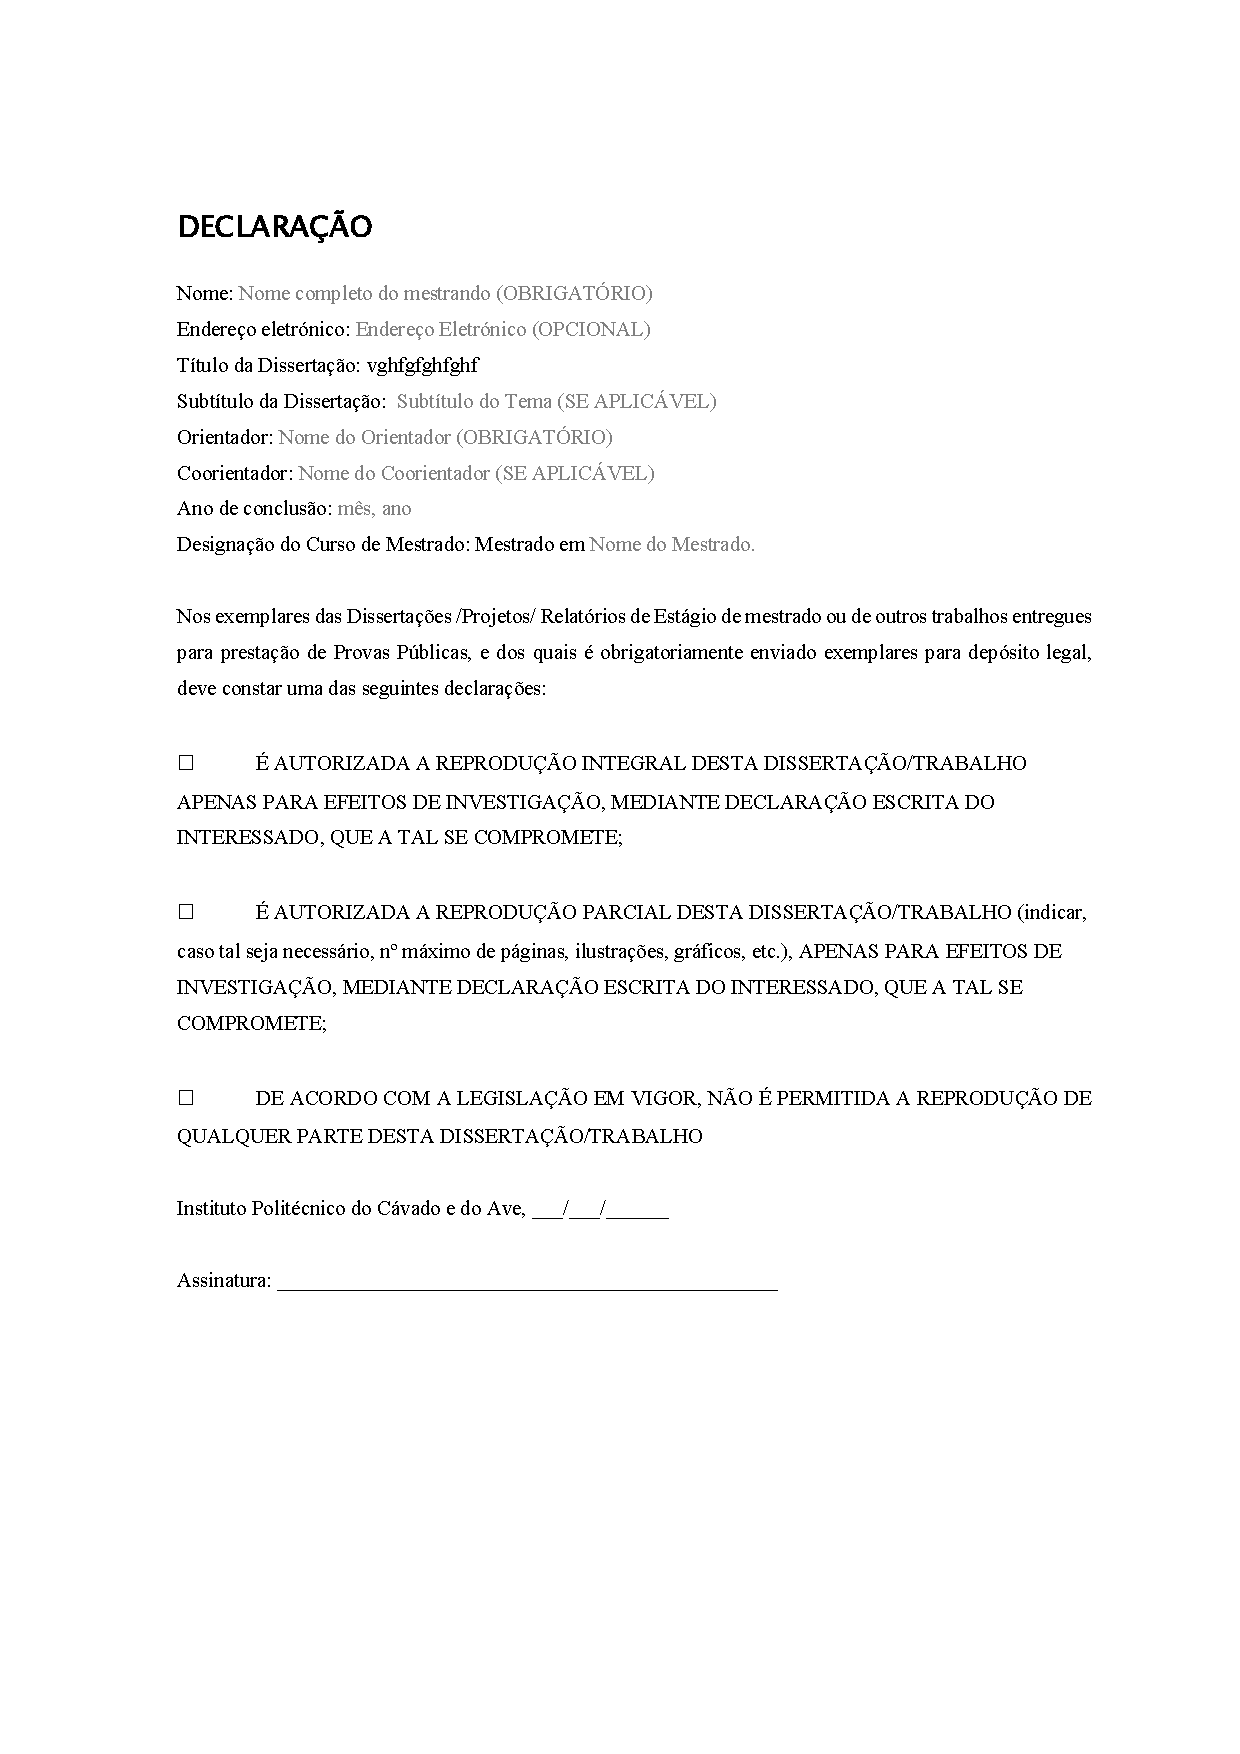
\includepdf[page={1}]{FrontCover/Declaration.pdf} \cleardoublepage
 \chapter*{Declaração}
\pagestyle{empty}

\noindent
\begin{tabular}{@{}ll}
Nome: & \textcolor{gray}{João Manuel Mesquita Fernandes} \\
Endereço eletrónico: & \textcolor{gray}{joaofernandes\_0398@outlook.pt} \\
Título da Dissertação: & \textcolor{gray}{Jersey Recognition and Team Affiliation on Soccer Game State Reconstruction} \\
Orientador: & \textcolor{gray}{José Brito} \\
Ano de conclusão: & \textcolor{gray}{Dezembro, 2026} \\
Designação do Curso: & \textcolor{gray}{Mestrado em Engenharia Eletrónica e de Computadores} \\
\end{tabular}

\vspace{0.8cm}

\noindent
Nos exemplares das Dissertações / Projetos / Relatórios de Estágio de mestrado ou de outros trabalhos entregues para prestação de Provas Públicas, e dos quais são obrigatoriamente enviados exemplares para depósito legal, deve constar uma das seguintes declarações:

\vspace{0.5cm}

\begin{itemize}[leftmargin=1.5cm, labelsep=0.3cm]
    \item[$\Box$] É AUTORIZADA A REPRODUÇÃO INTEGRAL DESTA DISSERTAÇÃO/TRABALHO APENAS PARA EFEITOS DE INVESTIGAÇÃO, MEDIANTE DECLARAÇÃO ESCRITA DO INTERESSADO, QUE A TAL SE COMPROMETE;
    
    \item[$\Box$] É AUTORIZADA A REPRODUÇÃO PARCIAL DESTA DISSERTAÇÃO/TRABALHO (indicar, caso tal seja necessário, nº máximo de páginas, ilustrações, gráficos, etc.), APENAS PARA EFEITOS DE INVESTIGAÇÃO, MEDIANTE DECLARAÇÃO ESCRITA DO INTERESSADO, QUE A TAL SE COMPROMETE;
    
    \item[$\Box$] DE ACORDO COM A LEGISLAÇÃO EM VIGOR, NÃO É PERMITIDA A REPRODUÇÃO DE QUALQUER PARTE DESTA DISSERTAÇÃO/TRABALHO.
\end{itemize}

\vspace{1cm}

\noindent
Instituto Politécnico do Cávado e do Ave, 07/12/2026 

\vspace{1cm}

\noindent
Assinatura: \underline{\hspace{9cm}} \cleardoublepage	% Edit the date, sign, create a PDF and replace it by the one on the previous line. Uncomment the previous line and comment this one

% #####################   Introductory Information     ###########################

{
\pagenumbering{Roman}

\begingroup
\begin{flushleft}
\bfseries
\fontfamily{phv}
{\Large
Jersey Recognition and Team Affiliation on Soccer Game State Reconstruction}

\mdseries
\end{flushleft}
\normalsize
\let\clearpage\relax
\chapter{RESUMO}
\endgroup

\noindent O SoccerNet é um \emph{benchmark} de visão computacional para a análise automática de jogos de futebol. O seu desafio de reconstrução do estado de jogo (\emph{Game State Reconstruction}, GSR) parte de um vídeo de uma única câmara. Para cada jogador, pede a posição no mapa do campo, a equipa, a função e o número da camisola. Na \emph{baseline} do desafio, a identificação dos jogadores tem dois pontos fracos. O número da camisola só fica certo em $15.3\%$ dos \emph{tracklets}, e a atribuição da equipa e do lado do campo falha em $28$ dos $159$ vídeos avaliados.

Este trabalho substituiu o módulo de reconhecimento do número, reescreveu os módulos da equipa e do lado do campo e acrescentou à reidentificação um descritor da cor do equipamento. Os restantes cinco módulos ficaram como na \emph{baseline}, para que qualquer diferença de desempenho possa ser atribuída às alterações feitas.

O número passou a ser lido pelo Qwen2.5-VL-3B, um modelo multimodal de visão e linguagem quantizado a 4 bits. O modelo lê apenas as costas do jogador, recortadas a partir da pose estimada. Cada leitura traz a confiança que o próprio modelo lhe atribui, e só as leituras seguras contam para a decisão. Esta regra reduziu os números errados para cerca de um terço. Na equipa, o agrupamento por aparência passou a verificar o próprio resultado e a recorrer à cor do equipamento quando a reidentificação não separa as equipas. O lado do campo passou a ser decidido por uma cascata de quatro critérios, o último dos quais usa o guarda-redes.

Nos $159$ vídeos anotados do SoccerNet-GSR, com a \emph{baseline} executada nas mesmas condições, a exatidão do número subiu de $15.3\%$ para $42.6\%$ dos \emph{tracklets}, e a da equipa e do lado de $83.5\%$ para $92.8\%$. O GS-HOTA, a métrica oficial do desafio, subiu de $31.30\%$ para $47.87\%$ no conjunto de teste, com ganhos da mesma ordem na validação e no treino, que não serviu para escolher nenhuma regra nem limiar. A decomposição da métrica por atributo mostra que todo o ganho vem do número e da equipa.

No número, o erro que resta deve-se sobretudo a algarismos que não se veem na imagem e ao \emph{tracking}, que parte jogadores em vários \emph{tracklets} e troca identidades. Na equipa, deve-se sobretudo a vinte vídeos de validação em que o classificador de função, que não foi alterado, confunde os jogadores de amarelo com árbitros.


\hspace{3cm}\\
\indent
\textbf{Palavras-chave: } Reconstrução do Estado de Jogo, Reconhecimento do Número da Camisola,
Atribuição da Equipa, Modelos Multimodais, SoccerNet
 \cleardoublepage
\begingroup
\begin{flushleft}
\bfseries
\fontfamily{phv}
{\Large
Jersey Recognition and Team Affiliation on Soccer Game State Reconstruction}

\mdseries
\end{flushleft}
\normalsize
\let\clearpage\relax
\chapter{ABSTRACT}
\endgroup

\noindent SoccerNet is a computer vision benchmark for the automatic analysis of football matches. Its Game State Reconstruction (GSR) challenge starts from a single-camera video. For each player, it asks for the position on the pitch map, the team, the role and the jersey number. In the challenge baseline, player identification has two weak points. The jersey number is correct in only 15.3\% of the tracklets, and team and pitch-side assignment fails in 28 of the 159 evaluated videos.

This work replaced the jersey number recognition module, rewrote the team and pitch-side modules and added a kit colour descriptor to the re-identification module. The other five modules were kept as in the baseline, so that any difference in performance can be attributed to the changes made.

The jersey number is now read by Qwen2.5-VL-3B, a multimodal vision-language model quantised to 4 bits. The model reads only the player's back, cropped from the estimated pose. Each reading comes with the confidence that the model itself assigns to it, and only confident readings count towards the decision. This rule reduced wrong numbers to about one third. In the team module, appearance-based clustering now checks its own result and falls back on kit colour when re-identification cannot separate the teams. The pitch side is now decided by a cascade of four criteria, the last of which uses the goalkeeper.

On the 159 annotated videos of SoccerNet-GSR, with the baseline run under the same conditions, jersey number accuracy rose from 15.3\% to 42.6\% of the tracklets, and team and pitch-side accuracy from 83.5\% to 92.8\%. GS-HOTA, the official challenge metric, rose from 31.30\% to 47.87\% on the test set, with gains of the same order on the validation and training sets. The training set was not used to choose any rule or threshold. Breaking the metric down by attribute shows that the whole gain comes from the jersey number and the team.

For the jersey number, the remaining error comes mostly from digits that are not visible in the image and from tracking, which splits players into several tracklets and swaps identities. For teams, it comes mostly from twenty validation videos in which the role classifier, which was not changed, mistakes the players in yellow for referees.


\hspace{3cm}\\
\indent
\textbf{Keywords: } Game State Reconstruction, Jersey Number Recognition, Team Affiliation, Multimodal Models, SoccerNet
 \cleardoublepage
\chapter{LISTA DE ABREVIATURAS E SIGLAS}

\vspace{1cm}

{
\setlength\arrayrulewidth{0pt}
\begin{tabular}{|l|l|l|}
\hline
AssA    & -- & Association Accuracy \\
CLAHE   & -- & Contrast Limited Adaptive Histogram Equalization \\
CNN     & -- & Convolutional Neural Network \\
CUDA    & -- & Compute Unified Device Architecture \\
DBSCAN  & -- & Density-Based Spatial Clustering of Applications with Noise \\
DetA    & -- & Detection Accuracy \\
FP4     & -- & 4-bit Floating Point \\
FPN     & -- & Feature Pyramid Network \\
GPU     & -- & Graphics Processing Unit \\
GSR     & -- & Game State Reconstruction \\
GS-HOTA & -- & Game State Higher Order Tracking Accuracy \\
HOTA    & -- & Higher Order Tracking Accuracy \\
HSV     & -- & Hue, Saturation, Value \\
IoU     & -- & Intersection over Union \\
IPCA    & -- & Instituto Politécnico do Cávado e do Ave \\
LocA    & -- & Localization Accuracy \\
OCR     & -- & Optical Character Recognition \\
pp      & -- & pontos percentuais \\
ReID    & -- & Re-Identification \\
ROI     & -- & Region of Interest \\
RPN     & -- & Region Proposal Network \\
VLM     & -- & Vision-Language Model \\
VRAM    & -- & Video Random-Access Memory \\
YOLO    & -- & You Only Look Once \\
\hline
\end{tabular}
}
 \cleardoublepage

\setcounter{tocdepth}{5}
\renewcommand{\contentsname}{ÍNDICE}
%\renewcommand{\contentsname}{TABLE OF CONTENTS}
\tableofcontents \cleardoublepage

\listoffigures 
\listoftables
\cleardoublepage

}

% ###############################################################
\pagenumbering{arabic}  											% Enable Regular Page Numbering
\restoregeometry

% ALTERADO: a numeracao passa a estar activa JA NA INTRODUCAO, para que esta
% seja o Capitulo 1. Antes, esta linha so aparecia depois da introducao.
\setcounter{secnumdepth}{5}											% Enable section numbering up to SubSubSection (level 5)

\chapter{Introdução}\label{cap:introducao}

O futebol é um dos desportos com maior projeção mediática e económica, e a análise dos jogos apoia-se cada vez mais em dados. Clubes e operadores televisivos usam-nos para estudar o comportamento das equipas, preparar os jogos com os adversários e fundamentar decisões táticas. Grande parte desses dados é, no entanto, anotada à mão por analistas. A outra parte vem de sistemas de várias câmaras instalados no estádio, caros e ao alcance de poucas competições. Obter a mesma informação de forma automática, a partir do vídeo da transmissão televisiva, que existe para a maioria dos jogos profissionais, tornaria esta análise mais rápida e mais acessível.

É neste contexto que se enquadra a reconstrução do estado de jogo (\emph{Game State Reconstruction}, GSR), formalizada por \citet{somers2024soccernet}. O objetivo é passar do vídeo de uma única câmara para um mapa do campo. Nesse mapa, cada interveniente aparece com a sua posição, a equipa, a função (jogador, guarda-redes ou árbitro) e o número da camisola. Para isso, o sistema resolve várias tarefas em cadeia. Primeiro, deteta as pessoas em cada \emph{frame} e segue-as ao longo do vídeo, com a ajuda da reidentificação quando um jogador fica tapado ou sai de imagem. Depois, calibra a câmara para projetar cada jogador no campo. Por fim, identifica cada um.

É nesta última etapa que se centra este trabalho. Inclui duas tarefas, o reconhecimento do número da camisola e a atribuição da equipa, e, em ambas, a imagem dá pouco com que trabalhar. Numa transmissão televisiva, o número ocupa poucos píxeis, aparece muitas vezes tapado ou de lado e só se lê em parte dos \emph{frames}. As cores dos equipamentos mudam com a luz e nem sempre contrastam o suficiente. O próprio artigo que propõe a tarefa aponta o número como a maior dificuldade da sua \emph{baseline} \citep{somers2024soccernet}. São, no entanto, estas duas tarefas que dão uma identidade a cada interveniente. Sem elas, o mapa mostra posições, mas não diz quem ocupa cada uma.

Os trabalhos sobre estas duas tarefas deixam ainda uma pergunta em aberto. Os métodos académicos são avaliados isoladamente, muitas vezes em conjuntos de dados próprios e fora do sistema completo. As soluções apresentadas ao desafio SoccerNet são avaliadas no sistema completo, mas alteram vários módulos ao mesmo tempo, e o ganho que obtêm não se consegue repartir pelas alterações feitas. Fica por saber quanto vale, sozinha, uma melhor identificação dos jogadores.

É a essa pergunta que esta dissertação procura responder. Na \emph{baseline} do desafio, o número da camisola só fica certo em $15.3\%$ dos \emph{tracklets}, e a atribuição da equipa e do lado do campo falha em $28$ dos $159$ vídeos avaliados. Para melhorar estas duas tarefas, alteram-se quatro dos nove módulos do \emph{pipeline}. O reconhecimento do número da camisola é substituído, e os módulos da equipa e do lado do campo são reescritos. A reidentificação ganha um descritor da cor do equipamento, sem que o seu modelo mude. Os outros cinco módulos, a deteção, o \emph{tracking}, os pontos do campo, a calibração e a agregação por \emph{tracklet}, ficam como na \emph{baseline}. Assim, qualquer diferença de desempenho resulta das alterações introduzidas.

No número da camisola, o MMOCR, o sistema de deteção e reconhecimento de texto usado pela \emph{baseline}, dá lugar a um modelo multimodal de visão e linguagem, o Qwen2.5-VL-3B. O modelo lê apenas as costas do jogador, recortadas a partir da pose estimada. As leituras de cada \emph{tracklet} são depois combinadas numa decisão única, em que só contam aquelas em que o próprio modelo diz estar seguro. Na equipa, o agrupamento por aparência passa a verificar o próprio resultado e a recorrer à cor do equipamento quando a reidentificação não separa as duas equipas. O lado do campo passa a ser decidido por uma cascata de quatro critérios, o último dos quais usa o guarda-redes. As regras e os limiares dos dois módulos são escolhidos nos conjuntos de teste e de validação. Na equipa, cada ajuste só é aceite se corrigir vídeos que falhavam sem estragar nenhum que a versão anterior já acertava.

O sistema proposto e a \emph{baseline} são executados nos mesmos $159$ vídeos anotados, nas mesmas condições e sobre os mesmos \emph{tracklets}. Antes de os comparar, foi preciso corrigir um defeito de calibração na configuração distribuída da \emph{baseline}, que não faz parte das alterações deste trabalho. A exatidão do número sobe de $15.3\%$ para $42.6\%$ dos \emph{tracklets}, e a da equipa e do lado sobe de $83.5\%$ para $92.8\%$. No GS-HOTA, a métrica oficial do desafio, o ganho é de $16.57$ pontos no conjunto de teste. A métrica é ainda decomposta por atributo, o que permite ler em separado o contributo do número e o da equipa. O conjunto de treino não serviu para escolher nenhuma regra nem limiar, e nele o GS-HOTA sobe $13.85$ pontos, um ganho da mesma ordem do teste.

Tão importante como os ganhos é perceber até onde vão. No número da camisola, as experiências feitas mostram que, nos casos mais difíceis, os algarismos não se veem na imagem, e nenhuma transformação do recorte os recupera. Outra fração do erro vem do \emph{tracking}, que divide jogadores em vários \emph{tracklets} e troca identidades, fora dos módulos alterados. Na equipa, a inspeção visual dos $159$ vídeos mostra que a maioria das falhas que restam vem do classificador de função. Em vinte vídeos da validação, este classificador dá como árbitros os jogadores de amarelo. A mesma inspeção mostra ainda que, em cinco vídeos, a própria anotação tem os lados invertidos.

\section{Objetivos e Contributos}\label{sec:objetivos}

O objetivo geral desta dissertação é quantificar o contributo da identificação dos jogadores para a reconstrução do estado de jogo. Para isso, propõem-se novas soluções para as duas tarefas de identificação da \emph{baseline} do SoccerNet-GSR. São elas o reconhecimento do número da camisola e a atribuição da equipa e do lado do campo. Os restantes módulos do \emph{pipeline} mantêm-se inalterados, com exceção da reidentificação, à qual se acrescenta um descritor de cor.

Deste objetivo geral decorrem três objetivos específicos. O primeiro é melhorar o reconhecimento do número da camisola sem treinar modelos nem anotar dados, dentro das limitações do \emph{hardware} disponível. O segundo é tornar a atribuição da equipa e do lado do campo fiável nos vídeos em que a \emph{baseline} falha. O terceiro é avaliar estas alterações de modo que o ganho obtido lhes possa ser atribuído sem ambiguidade, tanto em cada módulo como no sistema completo.

Do trabalho realizado resultam quatro contributos. O primeiro é um módulo de reconhecimento do número da camisola que dispensa treino específico. A estimativa de pose isola a região dorsal do jogador, e um modelo multimodal de visão e linguagem de pequena dimensão lê o recorte. A decisão de cada \emph{tracklet} usa apenas as leituras com confiança suficiente (Secção~\ref{sec:met-jnr}). O segundo é um método de atribuição da equipa que verifica a qualidade do agrupamento e recorre à cor do equipamento quando as características de reidentificação não separam as equipas. O lado do campo é depois determinado por uma cascata de critérios (Secção~\ref{sec:met-equipa}). Já o terceiro é um protocolo experimental que isola o efeito das alterações propostas. A \emph{baseline} e o sistema proposto são avaliados nas mesmas condições, e o GS-HOTA é decomposto por atributo (Capítulo~\ref{cap:resultados}). Por fim, o quarto é uma quantificação da fiabilidade da regra da posição média, usada para atribuir o lado do campo, sobre a anotação completa dos 160 vídeos. Esta análise, que os trabalhos revistos não fazem, revelou também cinco vídeos com os lados invertidos na própria anotação (Secção~\ref{sec:res_lado_quantificacao}).


\section{Estrutura do Documento}\label{sec:estrutura}

A dissertação está organizada em cinco capítulos. O presente capítulo enquadra o problema, delimita o âmbito do trabalho e enuncia os seus objetivos e contributos. O Capítulo~\ref{cap:estado-arte} revê o estado da arte sobre o reconhecimento do número da camisola e a atribuição da equipa, incluindo as soluções apresentadas ao desafio SoccerNet. Termina com as métricas de avaliação e as lacunas que motivam este trabalho. O Capítulo~\ref{cap:metodologia} descreve as alterações introduzidas nos quatro módulos, o ambiente experimental e o procedimento de avaliação. O Capítulo~\ref{cap:resultados} apresenta os resultados de cada módulo e o seu efeito no GS-HOTA, sempre em comparação com a \emph{baseline}. Por fim, o Capítulo~\ref{cap:conclusao} sintetiza os principais contributos e aponta direções de trabalho futuro. No final do documento, o Apêndice A reúne os resultados por vídeo dos dois sistemas.
 \cleardoublepage

% #################### Start of the Chapters ######################

\chapter{Estado da Arte}\label{cap:estado-arte}
Este capítulo revê o trabalho já feito nas duas tarefas em que a dissertação se foca, o reconhecimento do número da camisola e a atribuição da equipa de cada jogador. Antes de as abordar em detalhe, enquadra-se cada tarefa no \emph{pipeline} geral da reconstrução do estado de jogo e apresentam-se as métricas usadas, que servem tanto para avaliar o sistema completo como cada tarefa por si só. A revisão segue por temas, e não trabalho a trabalho, para clarificar as principais linhas de investigação e onde ainda falham.

\section{Reconstrução do Estado de Jogo}\label{sec:sistemas_gsr}

A reconstrução do estado de jogo, proposta por \citet{somers2024soccernet}, é uma tarefa de análise automática de vídeo desportivo, em particular no futebol. Os autores apresentaram a formulação do problema e disponibilizaram o \emph{dataset} SoccerNet-GSR e a arquitetura de referência. Na prática, o objetivo é converter um vídeo de uma única câmara, \emph{frame} a \emph{frame}, numa projeção bidimensional do terreno de jogo (Figura~\ref{fig:gsr-minimap}). Esta transformação implica detetar cada interveniente e acompanhá-lo ao longo do vídeo, localizar as linhas do campo para o situar no terreno e, por fim, identificar a equipa, a função e o número da camisola de cada um.

\begin{figure}[H]
    \centering
    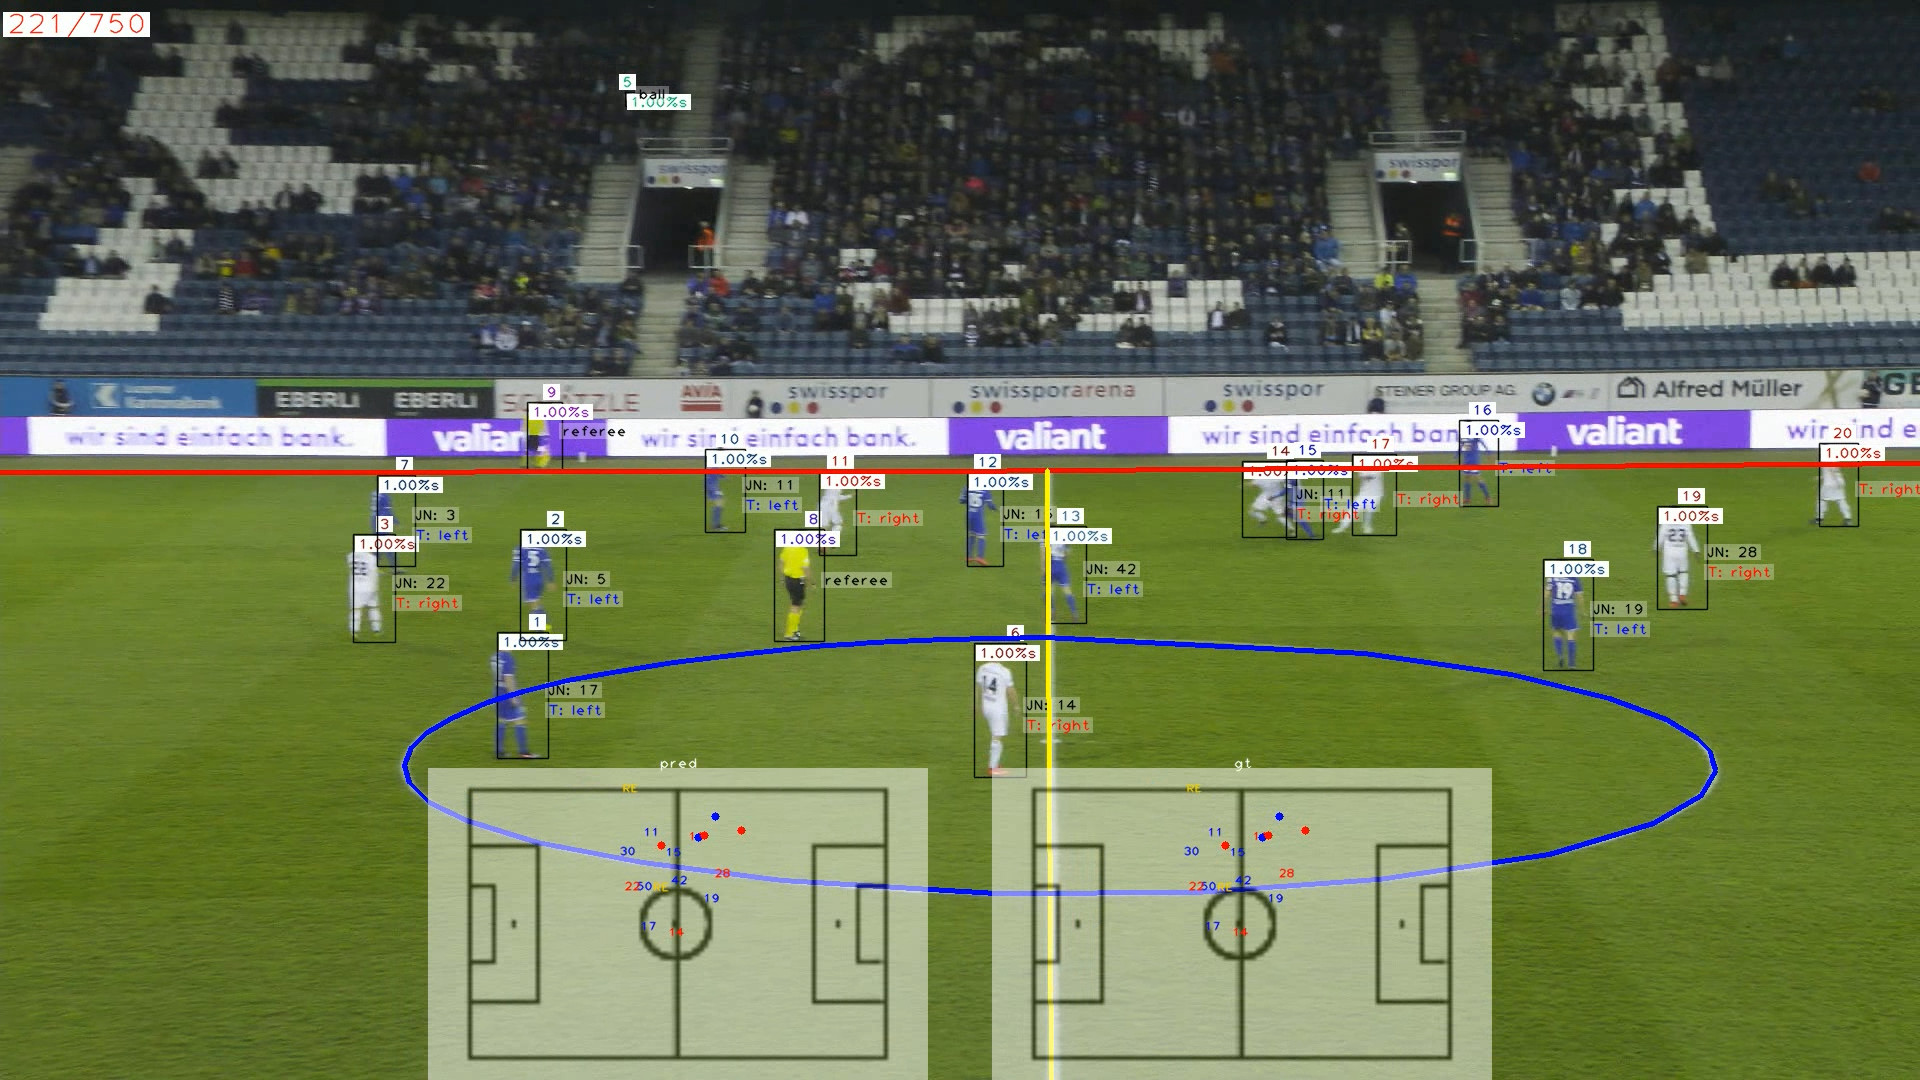
\includegraphics[width=0.8\textwidth]{gamestate-example.jpg}
    \caption{Exemplo de reconstrução do estado de jogo, com a posição, a equipa e o número da camisola projetados num mapa bidimensional do campo. Adaptado de \citet{somers2024soccernet}.}
    \label{fig:gsr-minimap}
\end{figure}

O \emph{dataset} SoccerNet-GSR é composto por sequências de 30 segundos, extraídas de transmissões televisivas de jogos profissionais. Cada sequência tem 750 \emph{frames}, a 25 imagens por segundo e com resolução de $1920 \times 1080$ píxeis. Está centrada numa ação do jogo, como um canto, um golo, um livre ou um fora de jogo. Em cada \emph{frame}, as pessoas estão anotadas com a caixa na imagem, definida pelas coordenadas do canto superior esquerdo, pela largura e pela altura, e com a posição no campo, em metros. A cada uma é atribuída uma função, que pode ser jogador, guarda-redes, árbitro ou outro. Os jogadores e os guarda-redes têm também a equipa. Nos jogadores, está ainda anotado o número da camisola, quando foi possível identificá-lo. A equipa não é dada pelo nome nem pela cor, mas pelo lado do campo, esquerdo ou direito, conforme a baliza que defende. Por fim, estão anotadas a bola e as linhas do campo. Nos 160 vídeos anotados usados neste trabalho, divididos em treino, validação e teste (Secção~\ref{sec:ambiente}), há cerca de 1.9 milhões de anotações de pessoas.  Existe também um subconjunto \emph{challenge}, sem anotação pública, sobre o qual o desafio apura as classificações.

A \emph{baseline} do SoccerNet-GSR, ponto de partida deste trabalho, é construída sobre o \emph{framework} TrackLab. Trata-se de uma estrutura modular que executa em sequência a deteção, a reidentificação e o \emph{tracking} dos jogadores, e a calibração da câmara (Figura~\ref{fig:gsr-pipeline}). Nesta estrutura, a identificação final é feita por três módulos. O primeiro é o modelo PRTreID, que extrai características ligadas à identidade, à equipa e à função de cada jogador. O segundo, a ferramenta MMOCR \citep{kuang2021mmocr}, lê os números das camisolas. O terceiro é um algoritmo de agrupamento (\emph{clustering}) que junta as representações visuais semelhantes para decidir a que equipa pertence cada jogador. Esta dissertação foca-se nestes dois últimos, por serem, entre os módulos de identificação, os que mais limitam o desempenho da \emph{baseline}.

\begin{figure}[H]
    \centering
    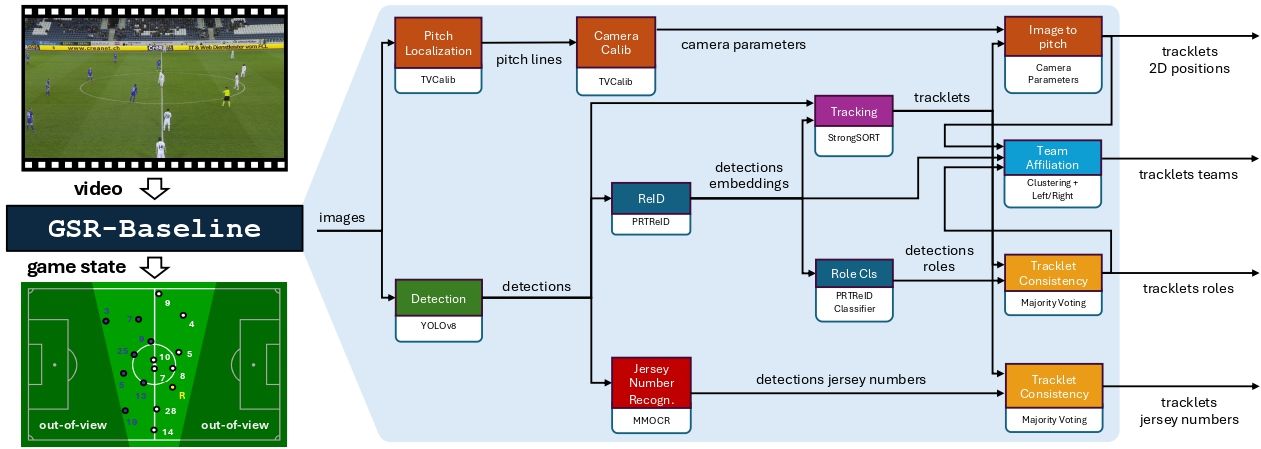
\includegraphics[width=\textwidth]{gsr_baseline_architecture.jpg}
    \caption{Arquitetura de referência do SoccerNet-GSR. Adaptado de \citet{somers2024soccernet}.}
    \label{fig:gsr-pipeline}
\end{figure}


Esta arquitetura modular tem, porém, um ponto fraco. O mapa só é útil se cada jogador estiver bem identificado, com o número da camisola, a equipa e a função certos, e não basta detetá-lo e segui-lo. Sem essa identificação, o mapa fica preenchido com posições sem identidade. As edições seguintes do desafio confirmam este diagnóstico \citep{cioppa2024soccernet, giancola2025soccernet}. A solução vencedora de 2024 \citep{golovkin2025minimap} segue, de forma independente, as duas ideias centrais desta dissertação. Na leitura do número, troca o OCR genérico por um modelo próprio para o futebol. Na equipa, junta a aparência à posição de cada jogador no campo. Há, no entanto, uma diferença de âmbito. Essa solução melhorou vários módulos ao mesmo tempo, da deteção à calibração, ao \emph{tracking} e ao pós-processamento. Esta dissertação altera apenas as duas tarefas de identificação. A deteção, o \emph{tracking} e a calibração ficam como na \emph{baseline}, e a reidentificação mantém o seu modelo, com um descritor de cor acrescentado para a atribuição da equipa. Assim, qualquer melhoria observada pode ser atribuída a estas alterações, e não a uma otimização global do sistema.

A reconstrução do estado de jogo é uma tarefa recente, disputada em apenas duas edições do desafio. Na primeira, em 2024, participaram dezasseis equipas com trinta e quatro submissões, e a solução vencedora elevou o GS-HOTA da \emph{baseline} de $23.36\%$ para $63.81\%$ \citep{cioppa2024soccernet}. Na segunda, em 2025, catorze equipas apresentaram sessenta e seis submissões sobre uma \emph{baseline} atualizada, com $29.01\%$, e a vencedora obteve $63.90\%$, com a solução vencedora de 2024 em segundo lugar, com o mesmo valor de $63.81\%$ \citep{giancola2025soccernet}. Deste historial, duas coisas contam para o que se segue. A primeira é que o valor máximo quase não se moveu entre as duas edições, apesar da mudança de paradigma na leitura do número, sinal de que a tarefa está longe de resolvida e de que nenhum módulo isolado a desbloqueia. A segunda é que os organizadores registam, na edição de 2025, três tendências comuns aos sistemas melhor classificados. São elas o recurso a características CLIP e OSNet para a reidentificação, a função e a equipa, o alisamento temporal da calibração por fluxo ótico, e a aplicação de modelos de visão e linguagem à leitura do número \citep{giancola2025soccernet}. A edição de 2026 do desafio já não incluiu a tarefa, substituída por cinco outras, entre as quais a deteção de ações centrada no jogador, que reutiliza a equipa e o número da camisola como identificadores \citep{cioppa2026soccernet}. Esta comparação é retomada no Capítulo~\ref{cap:resultados}, com a devida cautela, uma vez que o conjunto de teste usado neste trabalho não é o conjunto reservado em que o desafio apura as classificações.

\section{Reconhecimento do Número da Camisola}

O reconhecimento automático do número da camisola a partir de um vídeo de uma única câmara é difícil por razões que vêm da própria transmissão. A câmara está longe dos jogadores, e os algarismos ocupam poucos píxeis. Os jogadores correm, viram-se e tapam-se uns aos outros, e a camisola dobra-se com o movimento, pelo que o número raramente aparece de frente e legível. Os trabalhos publicados respondem a estas dificuldades de duas formas. Uns localizam e leem os dígitos em cada imagem, muitas vezes com a ajuda da pose. Outros aproveitam o facto de o mesmo jogador ser visto em muitas imagens e combinam as leituras ao longo do tempo. No fim da secção, descrevem-se as soluções apresentadas ao desafio SoccerNet.

\subsection{Abordagens por OCR Local e Modelos de Pose}

Os primeiros trabalhos abordaram a tarefa como um problema de deteção e classificação de dígitos. \citet{gerke2015soccer} foram dos primeiros a aplicar redes neuronais convolucionais (\emph{Convolutional Neural Networks}, CNN) ao reconhecimento do número da camisola, estabelecendo a viabilidade da abordagem. \citet{liu2019poseguided} deram um passo importante com uma R-CNN guiada por pose (\emph{pose-guided} R-CNN). Substituíram a \emph{Region Proposal Network} (RPN) tradicional por uma variante de três classes (fundo, pessoa e dígito) e usaram os \emph{keypoints} do corpo humano para refinar as propostas. Com isso, localizam melhor os dígitos, mesmo em poses difíceis. O modelo foi validado num conjunto de dados criado especificamente para o efeito, com anotações detalhadas de caixas de pessoa e de dígito.

Esta linha foi consolidada por \citet{liu2022jede} com o JEDE, um detetor universal que combina uma \emph{Feature Pyramid Network} (FPN) com uma \emph{Region Proposal Network} (RPN) e um ramo guiado por pose (\emph{pose-guided branch}) para as propostas de dígitos. Testado em futebol e basquetebol, superou métodos clássicos como o Faster R-CNN e o Mask TextSpotter, sobretudo na precisão e revocação da deteção.

Mais recentemente, \citet{koshkina2024general} propuseram uma abordagem distinta, que trata o reconhecimento do número como um caso de reconhecimento de texto em cena (\emph{scene text recognition}). Em vez de detetar cada dígito isoladamente, encadeiam um classificador de legibilidade (\emph{legibility classifier}), que descarta os \emph{frames} onde o número não está legível, com um modelo de reconhecimento de texto, agregando depois as leituras ao longo do \emph{tracklet}. Os autores disponibilizam ainda um conjunto de dados público, com anotações de legibilidade, e avaliam o desempenho tanto ao nível da imagem como do \emph{tracklet}. Ao escolher primeiro as imagens úteis e decidir depois ao longo do \emph{tracklet}, esta estratégia aproxima-se da adotada nesta dissertação. A diferença está nos meios. Os autores usam um classificador de legibilidade treinado à parte e um leitor de texto convencional. Este trabalho usa um modelo de visão e linguagem e a confiança que ele próprio atribui a cada leitura. Além disso, a abordagem dos autores é avaliada de forma isolada e num conjunto de dados próprio, e não dentro do \emph{pipeline} completo da reconstrução do estado de jogo.

\subsection{Abordagens temporais e por \emph{keyframes}}

Uma linha de investigação diferente tira partido do tempo, uma vez que a mesma camisola é vista em muitos \emph{frames}, mas só está legível em alguns. A ideia é escolher os bons em vez de ler todos. \citet{balaji2023jersey} apresentam uma rede espácio-temporal com um módulo que identifica os \emph{frames}-chave (\emph{keyframes}), aqueles em que o número aparece com mais nitidez, e concentram neles a leitura. O número é reconhecido por classificação, ou seja, a rede parte de uma lista fechada de números possíveis, fixada no treino, e escolhe um deles. É treinada com uma função de perda que junta num só objetivo a escolha dos \emph{keyframes} e o reconhecimento do número (\emph{multi-task loss}). A abordagem aguenta bem as oclusões e o movimento rápido, mas tem uma limitação que os próprios autores reconhecem, a de tratar o número como um todo, e não dígito a dígito.

O trabalho seguinte da mesma equipa, \citet{balaji2024dmae}, muda o foco. Em vez de escolher os melhores \emph{frames}, procura extrair de cada recorte características mais robustas, que aguentem a baixa resolução. Para isso recorre a um \emph{masked autoencoder}, uma rede que aprende sozinha, sem rótulos, tapando pedaços da imagem e treinando-se a reconstruí-los, o que a obriga a perceber a estrutura do que está a ver. O «\emph{domain-guided}» do nome vem de esse treino ser feito de propósito com imagens desfocadas por movimento, para se parecerem com as de uma transmissão real, e as leituras dos vários \emph{frames} são depois combinadas ao longo do tempo por um descodificador \emph{transformer}. Os ganhos que apresentam são modestos, mas reforçam a ideia que atravessa toda esta linha de trabalho. Em baixa resolução, a cor do equipamento não chega, e é preciso extrair da imagem características mais profundas para distinguir dígitos pequenos.

Nenhuma destas duas propostas foi seguida neste trabalho, e a razão é a mesma nas duas. Ambas assentam em modelos que é preciso treinar sobre imagens anotadas, o módulo de \emph{keyframes} num caso e o d-MAE no outro, e aqui não se treinou nenhum modelo nem se anotaram dados, até porque tudo tinha de encaixar na \emph{baseline} sem voltar a treinar as etapas anteriores. Ainda assim, a ideia que lhes está por trás, ler o número só onde ele se vê bem e juntar as leituras ao longo do tempo, é boa e foi aproveitada, mas por um caminho mais simples. Em vez de confiar a escolha dos \emph{frames} a um modelo treinado, escolhem-se em cada janela os recortes mais nítidos e contam só as leituras em que o próprio modelo se mostra seguro (Secção~\ref{sec:met-jnr}).

\subsection{Soluções submetidas ao desafio SoccerNet}\label{sec:jnr-desafio}

Os trabalhos analisados até aqui são artigos científicos, publicados e avaliados. Existe, porém, outro tipo de trabalho que não passa por essa avaliação, as soluções que concorreram às várias edições do desafio SoccerNet, descritas apenas nos relatórios oficiais. Para esta dissertação, são as fontes mais úteis. O que se extrai destas soluções não é apenas a classificação que alcançaram, mas também as escolhas técnicas que revelam. A leitura dos relatórios mostra, de forma geral, uma mudança do OCR tradicional para os modelos de visão e linguagem ao longo das três edições, de 2023 a 2025. As descrições que se seguem resumem o que as próprias equipas escreveram nesses relatórios \citep{cioppa2023soccernet, cioppa2024soccernet, giancola2025soccernet}, exceto quando se cita o artigo completo de uma delas.

Na edição de 2023, o reconhecimento do número foi disputado como uma tarefa à parte. Cada exemplo era um \emph{tracklet}, isto é, uma sequência de pequenos recortes do mesmo jogador retirada dos vídeos do SoccerNet-Tracking, e o objetivo era dizer que número, de 1 a 99, esse jogador tinha na camisola, ou responder $-1$ quando o número nunca chegava a ser visível. Os organizadores disponibilizaram 2853 \emph{tracklets} anotados, e a avaliação final foi feita sobre outros 1211, pela exatidão, ou seja, a percentagem de \emph{tracklets} com a resposta certa. Participaram quinze equipas, com 157 submissões, e a melhor chegou a $92{.}85\%$. Estes valores não são comparáveis com os desta dissertação. No desafio, os \emph{tracklets} já vinham feitos e só se media a leitura do número. Aqui, o número é um dos atributos do \emph{pipeline} completo, os \emph{tracklets} saem do próprio \emph{tracking}, com os seus erros, e a métrica é o GS-HOTA, que avalia ao mesmo tempo a deteção, o \emph{tracking} e a identificação de cada jogador.

Desta edição aproveita-se o método. Segundo os organizadores, a maioria das equipas resolveu o problema em três etapas. Primeiro, um detetor de texto, como o DBNet++, o MMOCR, o DeepSolo ou o YOLO, localiza o número em cada recorte. Depois, um modelo de OCR afinado para o efeito, tipicamente o PP-OCRv3 ou o PaddleOCR, lê o número identificado. Por fim, uma votação maioritária junta as leituras de todos os recortes do \emph{tracklet} em apenas uma resposta. A equipa vencedora seguiu o mesmo esquema e investiu sobretudo no treino. Usou o detetor de texto para retirar dos dados de treino as imagens sem número visível, aumentou esses dados com rotações, inversões, mudanças de escala, ruído e sobreposição de vários \emph{frames}, treinou cinco modelos de reconhecimento de texto diferentes e juntou os votos de todos. Daqui tiram-se duas lições. A primeira é que a votação ao longo do \emph{tracklet} já era prática corrente em 2023, e não é por isso uma novidade deste trabalho, que a aplica apenas às leituras em que o modelo está seguro. A segunda é que todas estas soluções dependem de afinar modelos de OCR com os \emph{tracklets} anotados do próprio desafio, e é precisamente esse treino que a abordagem da Secção~\ref{sec:met-jnr} dispensa.


Em 2024, na primeira edição da reconstrução do estado de jogo, o número deixou de ser uma tarefa à parte. Passou a ser um dos atributos que cada sistema tinha de identificar a partir dos seus próprios \emph{tracklets}. Viu-se assim uma mudança de abordagem, em que as equipas melhor classificadas trocaram o OCR genérico por modelos próprios, treinados só para o número da camisola.

\citet{golovkin2025minimap} dividem as soluções em dois grupos. O primeiro adapta técnicas de OCR de uso geral, que localizam o texto antes de o ler e perdem exatidão com jogadores distantes, com oclusões e com jogadores virados de lado. Já o segundo usa soluções desenhadas para o futebol, que são mais exatas, mas precisam de treino específico para cada conjunto de dados.

A solução vencedora, que é a dos próprios autores, é um bom exemplo do segundo grupo. Em vez de detetar cada dígito com uma caixa, usa uma rede residual modificada que recebe recortes de $32\times32$ píxeis e tem duas cabeças de classificação, uma que prevê o algarismo das dezenas, ou que ele não existe, e outra que prevê o das unidades. Assim, consegue ler o número mesmo quando parte dele está tapada, e não é preciso anotar uma caixa à volta de cada dígito. A equipa UPCxMobius, com a solução \emph{No bells, More Whistles}, que ficou em segundo lugar \citep[equipa GSR-2]{cioppa2024soccernet}, seguiu um caminho parecido e treinou um detetor de dígitos com dados públicos e cerca de mil \emph{frames} anotados de propósito. A equipa \emph{playbox x NUSG} \citep[equipa GSR-14]{cioppa2024soccernet} usou o CLIP em duas fases, com um modelo a decidir se há número visível e outro a dizer qual é, afinados sobre três mil caixas anotadas à mão, mas no conjunto final do desafio não chegou a superar a \emph{baseline}. O que estas soluções têm em comum é o custo de anotação. Cada uma teve de construir o seu próprio conjunto de treino, um esforço que as condições desta dissertação não permitiam.

A edição de 2025 marca uma mudança clara. Os organizadores referem, no relatório final dos resultados, que os modelos de visão e linguagem foram aplicados com sucesso à leitura do número. Destacam o LLaMA-3.2-Vision \citep{grattafiori2024llama3} e o Qwen2-VL-Instruct \citep{wang2024qwen2vl}. O primeiro foi utilizado pela equipa vencedora, a KIST \citep[equipa GSR-1]{giancola2025soccernet}, cujo sistema é descrito em detalhe por \citet{oo2026broadcast2pitch}. Os autores tratam a identificação completa do jogador como uma tarefa de geração autorregressiva multimodal. Em vez de treinarem um classificador por atributo, dão ao modelo o recorte do jogador com uma instrução em linguagem natural que lhe pede a função, o número e a cor da camisola, e leem a resposta como uma sequência de \emph{tokens}. Justificam a escolha com três vantagens. A primeira é generalizar melhor a atributos nunca vistos, como cores de camisola novas, o que é essencial para um reconhecimento aberto. A segunda é exigir menos anotação e menos engenharia, porque basta ajustar a instrução para pedir outras tarefas, sem mudar a arquitetura. A terceira é poder adaptar-se a outros ambientes desportivos e formatos de jogo. O Qwen2-VL-Instruct foi usado de outra forma pela equipa eidos.ai, sétima classificada \citep[equipa GSR-7]{giancola2025soccernet}. Em vez de classificar cada deteção à parte, mostra ao modelo uma longa sequência de deteções organizadas numa grelha e pede-lhe que raciocine passo a passo antes de responder.

O artigo de \citet{oo2026broadcast2pitch} traz ainda a comparação mais direta entre abordagens encontrada na literatura, porque testa três modelos de identificação dentro do mesmo \emph{pipeline} e sobre o mesmo conjunto de teste. Como primeira abordagem, junta modelos especializados por atributo, o PRTreID para a função, o EasyOCR para o número e uma ResNet-18 para a cor da camisola, e com isso obtém $18{.}11\%$ de GS-HOTA. Já a segunda abordagem usa o CLIP como codificador, com uma cabeça de classificação para cada atributo, e chega a $60{.}13\%$. Por fim, a terceira abordagem, com o LLaMA-3.2-Vision, sobe ligeiramente para $61{.}48\%$. Como o resto do sistema é igual nas três configurações, a diferença vem só do módulo de identificação. Não se pode atribuir apenas ao número, porque esse módulo decide também a função e a equipa, mas uma distância de mais de quarenta pontos deixa claro que os modelos de visão e linguagem identificam o jogador muito melhor do que um conjunto de modelos separados. Os autores reconhecem, ainda assim, que a vantagem do LLaMA-3.2-Vision sobre o CLIP é pequena e tem um custo computacional maior. Em sentido contrário, a equipa Playbox \& MIXI, quarta classificada \citep[equipa GSR-4]{giancola2025soccernet}, manteve o reconhecimento de texto convencional. Isola primeiro o tronco do jogador com os pontos do ViTPose e só depois lê o número com o PARSeq, os mesmos passos do método de \citet{koshkina2024general}. É a ideia de recorte orientado pela pose que este trabalho também usa (Secção~\ref{sec:met-jnr}), aqui ligada a um OCR clássico, o que indica que o OCR ainda tem lugar entre os melhores sistemas quando recebe a região certa da camisola.

Mais do que um trabalho aponta o número da camisola como o atributo mais difícil de todo o sistema. Por exemplo, a UTokyo Football Lab, da Universidade de Tóquio \citep[equipa GSR-8]{giancola2025soccernet}, termina a sua descrição a reconhecer que, tal como na \emph{baseline}, a maior dificuldade esteve no reconhecimento do número, e aponta os modelos multimodais como o passo seguinte. A prova mais completa vem, outra vez, de \citet{oo2026broadcast2pitch}, que calculam a métrica oficial juntando um atributo de cada vez à posição, dentro do seu próprio sistema. Só com a posição no campo, o GS-HOTA chega a $79{.}52\%$. Com a função, quase não muda e fica em $79{.}20\%$. Com a equipa, desce para $73{.}58\%$, ou para $77{.}39\%$ sem três vídeos em que a equipa está mal anotada. Com o número da camisola, cai para $64{.}70\%$, e com todos os atributos juntos fica em $61{.}48\%$. O número é, portanto, o atributo que mais custa ao sistema, com uma perda de quase quinze pontos. Os autores explicam-no pela própria transmissão televisiva, em que os dígitos aparecem desfocados, tapados ou visíveis em poucos \emph{frames} de cada \emph{tracklet}. Acrescentam que a votação maioritária por \emph{tracklet} se torna frágil quando as leituras certas são poucas, problema que a votação restrita às leituras seguras procura atenuar (Secção~\ref{sec:met-jnr}). É uma confirmação externa, e com números, da premissa de que esta dissertação parte. Nos mesmos dados, a equipa é o segundo atributo que mais custa, bem à frente da função, o que justifica que sejam o número e a equipa os dois atributos em que este trabalho intervém.


\section{Atribuição da equipa}

A atribuição da equipa consiste em decidir a que equipa cada jogador pertence. Na maior parte dos trabalhos, essa decisão faz-se com base na aparência, seja pela cor do equipamento, seja por características aprendidas por uma rede neuronal. Os métodos diferenciam-se sobretudo pela informação que usam para separar as duas equipas. 
Na reconstrução do estado de jogo há ainda um segundo passo, pois não é suficiente separar os jogadores em dois grupos. Também é necessário determinar qual das equipas defende a baliza da esquerda e qual defende a da direita. As subsecções seguintes começam pelos métodos baseados na cor, passam pelos que aprendem as características a partir dos dados e terminam nas soluções submetidas ao desafio SoccerNet, onde surge a questão do lado do campo.
\subsection{Métodos baseados em cor}

Os métodos mais simples usam a cor do equipamento para separar as equipas. As próprias Leis do Jogo ajudam nesta tarefa, pois obrigam as duas equipas a vestir cores que as distingam uma da outra e da equipa de arbitragem. Por isso, para quem vê o jogo, a cor chega quase sempre para distinguir as duas equipas. A exceção é o guarda-redes, que tem de usar uma cor diferente da de todos os outros jogadores, incluindo os da sua própria equipa. Assim, só pela cor, não há forma de saber a que equipa ele pertence. Num sistema automático, a cor é menos fiável do que parece, porque a mesma camisola muda de tom com a luz e a sombra, fica desfocada quando o jogador corre e, nos jogadores mais distantes, ocupa poucos píxeis.

O DeepPlayer-Track, de \citet{naik2022deepplayer}, mostra como esta abordagem funciona na prática. Cada jogador detetado é atribuído a uma das equipas, ou ao árbitro, apenas pela cor da camisola, e essa atribuição é depois usada para seguir os jogadores ao longo do vídeo sem que troquem de identidade. É um caso útil para esta dissertação por duas razões. Foi testado, entre outros, em transmissões televisivas do SoccerNet, o mesmo tipo de vídeo usado neste trabalho, e os autores mostram, com exemplos, onde a separação pela cor falha. O sistema funciona em duas etapas. Na primeira, um detetor YOLOv4 encontra em cada \emph{frame} os jogadores, a bola e o árbitro, e trata como fundo tudo o que está fora do campo. Na segunda, cada caixa é classificada pela cor, comparando os seus píxeis com três gamas de cor que os autores escolheram à mão a partir dos próprios vídeos, uma para a equipa de branco, outra para a de azul e outra para o árbitro, de vermelho. Essa classificação entra depois no \emph{tracker}, o JCD-SORT, uma variante do SORT. Para decidir a que trajetória pertence cada nova deteção, o \emph{tracker} combina a cor com a distância do cosseno entre descritores de aparência extraídos por uma rede convolucional. Com isso, dois jogadores de equipas diferentes dificilmente trocam de identidade, mesmo quando se cruzam.

O trabalho mostra que, com as gamas certas, a cor chega para separar as duas equipas e o árbitro. O ponto fraco está em essas gamas serem escolhidas à mão e só servirem nos vídeos em que foram escolhidas. Os próprios autores apresentam um vídeo do SoccerNet em que o árbitro não veste de vermelho, e o sistema, que só o reconhece por essa cor, trata-o como mais um jogador. Reconhecem também que a cor não resolve as trocas entre jogadores da mesma equipa, que continuam a acontecer quando um tapa o outro, e propõem, como trabalho futuro, reconhecer o número da camisola para os distinguir. Um método com as cores definidas à partida tem, portanto, de ser reconfigurado para cada jogo e falha sempre que alguém em campo vestir uma cor que não estava prevista. É precisamente essa configuração manual que este trabalho pretende evitar.

O PlayerTV, de \citet{solberg2024playertv}, reduz essa configuração ao mínimo e combina a cor com outra característica do jogador. Este sistema gera automaticamente resumos com os lances de cada jogador e, para isso, precisa de saber a equipa e o número de cada um. A equipa vem da cor, mas sem gamas fixas. Para cada \emph{tracklet}, calcula-se a cor média de uma região da metade de cima do jogador, cortando os lados para deixar de fora a relva. Essas cores são divididas em dois grupos pelo \emph{k-means}, e cada \emph{tracklet} fica na equipa do grupo mais próximo. Os grupos são aprendidos em cada vídeo, e a única informação de cor dada à partida é uma base de dados com as cores do equipamento principal e alternativo de cada equipa da liga, que serve apenas para dar nome a cada grupo. Essa outra característica é o número da camisola. Quando o número lido é mais seguro do que a cor, e ainda não está atribuído na outra equipa, é o número que decide a equipa. Em 16 vídeos da liga norueguesa, com 511 \emph{tracklets} anotados, a equipa fica certa em $91{.}5\%$ dos casos no espaço de cor CIELAB, e em $93{.}7\%$ depois do pós-processamento. O número, pelo contrário, só é lido corretamente em cerca de $30\%$ dos \emph{tracklets}, e os autores apontam-no como a principal limitação do sistema. Por procurar apenas dois grupos, um para cada equipa, o método também não identifica o árbitro.

Já \citet{pan2024unsupervised} vão mais longe e usam apenas a cor, sem nenhuma informação dada à partida, num método avaliado no SoccerNet-GSR, o mesmo conjunto de dados desta dissertação. O problema de que tratam é o da luz, porque nos jogos ao ar livre a mesma camisola pode parecer de duas cores diferentes conforme o jogador está ao sol ou à sombra. Por isso, antes de agrupar as pessoas pelas suas cores dominantes, o método corrige as sombras da imagem. No SoccerNet-GSR, chega a uma exatidão de $85{.}4\%$. Os próprios autores reconhecem, no entanto, duas limitações. Os grupos são formados imagem a imagem, sem ligação ao longo do vídeo, e o método ainda não chega aos cinco papéis que pretendem, as duas equipas, os dois guarda-redes e o árbitro, para o que propõem juntar à cor a posição dos jogadores no campo.

Os três trabalhos mostram que a cor separa bem as equipas. O que muda de um para o outro é quanto é preciso configurar à mão. O DeepPlayer-Track precisa de gamas de cor escolhidas para cada jogo. O PlayerTV aprende os grupos em cada vídeo, mas usa uma base de dados para lhes dar nome. O método de \citet{pan2024unsupervised} dispensa as duas coisas. Nenhum deles resolve, no entanto, o guarda-redes, e nenhum chega ao segundo passo, o de dizer que equipa defende cada baliza. O PlayerTV deixa ainda uma confirmação útil para esta dissertação. Com uma solução tão simples como a cor média, a equipa fica certa em mais de $90\%$ dos \emph{tracklets}, mas o número da camisola fica pelos $30\%$, o que volta a mostrar que é no número que está a maior dificuldade. Este trabalho segue a mesma ideia de aprender a separação em cada vídeo, sem nada configurado à mão, mas com características aprendidas em vez da cor, o tipo de abordagem tratado na subsecção seguinte.

\subsection{Métodos por aprendizagem e agrupamento}

Para ganhar robustez, outros trabalhos substituem a cor por características aprendidas por redes neuronais. A ideia comum é representar cada jogador por um vetor de características, de modo que a distância entre jogadores de equipas diferentes seja maior do que entre jogadores da mesma equipa. A rede é treinada uma única vez, e em cada jogo basta agrupar esses vetores, o que permite lidar com equipas e equipamentos que a rede nunca viu. Os trabalhos distinguem-se sobretudo no modo como essa representação é aprendida.

O trabalho de \citet{alhejaily2023team} é o exemplo mais simples destes métodos, porque a rede não é treinada para separar equipas. Os autores usam um \emph{autoencoder} convolucional, uma rede com duas metades. A primeira resume a imagem num vetor pequeno, e a segunda tenta reconstruir a imagem original apenas a partir desse vetor. O treino consiste em comparar a imagem reconstruída com a original e em corrigir a rede para que fiquem cada vez mais parecidas, o que dispensa qualquer rótulo. A rede é treinada uma vez sobre o Tiny ImageNet, um conjunto de imagens genéricas que nem sequer são de futebol. Depois de treinada, usa-se só a primeira metade, para transformar o recorte de cada pessoa num vetor, e a separação das equipas fica a cargo do \emph{k-means}, refeito em cada vídeo. Para isso, os autores escolhem 100 \emph{frames} ao acaso, detetam as pessoas com um detetor YOLOv3, passam cada recorte pela rede e dividem os vetores resultantes em três grupos, um para cada equipa e um terceiro para os guarda-redes e os árbitros. A partir daí, cada jogador fica no grupo cujo centro está mais próximo do seu vetor. Em 100 \emph{frames} anotados à mão, o método acerta em $92\%$ dos casos. Com o mesmo \emph{k-means} aplicado diretamente às cores dos recortes, acerta em $86\%$. A vantagem é não precisar de nenhum dado de futebol anotado. O preço é que o vetor guarda tudo o que é preciso para reconstruir a imagem, incluindo a luz e a sombra, e não apenas o que distingue as equipas. \citet{pan2024unsupervised} mostram precisamente que, com luz irregular, este método pode pôr os jogadores que estão à sombra num grupo à parte.

\citet{istasse2019associative} seguem o caminho oposto e treinam a rede precisamente para separar equipas, em imagens de basquetebol. A rede trabalha sobre a imagem inteira, e não sobre recortes de jogadores. Segmenta os jogadores, tratando os árbitros como fundo, e atribui a cada píxel um vetor, aprendido de modo a ser parecido entre jogadores da mesma equipa e diferente entre as duas equipas da mesma imagem. Como aprende a separar as equipas presentes em cada imagem, e não a reconhecer cores concretas, não precisa de ser treinada de novo para cada jogo, embora o treino inicial exija imagens anotadas com a equipa de cada jogador. Em jogos e pavilhões que não viu no treino, atribui a equipa certa a mais de $90\%$ dos jogadores, contra $62\%$ de um agrupamento por histogramas de cor. A decisão é, no entanto, tomada imagem a imagem, sem \emph{tracklets} nem ligação entre imagens seguidas do vídeo.

\citet{koshkina2021contrastive} treinam uma representação do mesmo tipo sem nenhum rótulo de equipa, em vídeos de hóquei no gelo filmados por uma câmara fixa que apanha o rinque inteiro. Usam aprendizagem contrastiva (\emph{contrastive learning}), em que a rede aprende a aproximar exemplos do mesmo grupo e a afastar os de grupos diferentes. Como não há rótulos, os grupos de partida vêm da cor, e só os jogadores agrupados com mais segurança servem de exemplos para o treino. Ao contrário do trabalho anterior, a rede trabalha sobre o recorte de cada jogador detetado. Num jogo novo, os recortes dos primeiros \emph{frames} chegam para encontrar os centros das duas equipas, e a partir daí cada jogador detetado fica na equipa do centro mais próximo. Com um único \emph{frame}, a equipa fica certa em $94\%$ dos casos, e com 500 \emph{frames}, cerca de 17 segundos de jogo, em $97\%$. O árbitro é identificado à parte, por um classificador treinado com exemplos anotados. Tal como no trabalho anterior, não há \emph{tracklets}, e cada deteção é decidida isoladamente.

A mesma ideia está no PRTreID, de \citet{mansourian2023multitask}, a rede cujas representações a \emph{baseline} usa para atribuir a equipa. O PRTreID é uma rede de reidentificação, treinada com recortes de jogadores do SoccerNet, que aprende três tarefas ao mesmo tempo. Reconhece a mesma pessoa em imagens diferentes, classifica a sua função e separa as equipas. Na tarefa da equipa, todos os recortes de cada lote de treino vêm do mesmo vídeo, e a rede aprende a aproximar jogadores da mesma equipa e a afastar os da equipa adversária. Tal como em \citet{istasse2019associative}, a comparação faz-se sempre dentro do mesmo jogo, e por isso a rede não aprende nenhuma equipa em concreto e pode ser usada em qualquer jogo. Esta tarefa usa apenas jogadores de campo, ficando de fora os guarda-redes, os árbitros e os restantes elementos. Os autores medem o seu efeito dividindo os jogadores de cada vídeo em dois grupos pelo \emph{k-means}. Com a rede treinada só para reidentificação, a equipa fica certa em $91{.}87\%$ dos casos, e com as três tarefas em conjunto sobe para $95{.}6\%$.

A \emph{baseline} \citep{somers2024soccernet} usa estas representações com uma diferença importante em relação aos trabalhos desta subsecção. Em vez de decidir a equipa imagem a imagem ou deteção a deteção, decide-a por \emph{tracklet}. Para cada \emph{tracklet} com a função de jogador, faz-se a média das representações do PRTreID de todas as suas deteções, o que dá um único vetor por \emph{tracklet}. Esses vetores são divididos em dois grupos pelo \emph{k-means}, e todas as deteções de um \emph{tracklet} recebem a equipa do seu grupo. Por fim, o lado de cada grupo decide-se pela posição média dos seus jogadores no campo, um passo que se discute na subsecção seguinte.

Os vetores de características aprendidos por uma rede neuronal separam melhor as equipas do que a cor, como mostram as comparações de \citet{alhejaily2023team}, com $92\%$ contra $86\%$, e de \citet{istasse2019associative}, com $90\%$ contra $62\%$. Todos estes métodos tratam, no entanto, o guarda-redes e o árbitro à parte, e só a \emph{baseline} decide por \emph{tracklet} e chega ao lado do campo. Este trabalho parte dessa mesma base, os vetores do PRTreID agrupados por \emph{tracklet} em cada vídeo, e recorre à cor apenas nos vídeos em que esses vetores não separam bem as duas equipas, como se descreve no Capítulo~\ref{cap:metodologia}.

\subsection{Soluções submetidas ao desafio SoccerNet}\label{sec:equipa-desafio}

Ao contrário da maioria dos trabalhos anteriores, as soluções submetidas ao desafio têm de resolver os dois passos, porque a métrica oficial exige que cada jogador seja identificado como pertencendo à equipa da esquerda ou à da direita. Esta subsecção descreve primeiro como separam as equipas e depois como decidem o lado, que é onde mais divergem.

Para o primeiro passo, \citet{golovkin2025minimap} descrevem uma estrutura comum à maioria dos sistemas, a mesma das subsecções anteriores. Cada jogador é descrito por um histograma de cor ou por um vetor de reidentificação, e esses vetores são agrupados pelo \emph{k-means} ou pelo DBSCAN em dois a cinco grupos, conforme se separam só as duas equipas ou também os árbitros e os guarda-redes. A solução vencedora de 2024, que é a dos próprios autores, segue esta estrutura com dois cuidados. Os vetores vêm de uma OSNet treinada para distinguir 111 equipamentos diferentes, e os grupos são cinco, as duas equipas, os árbitros e os dois guarda-redes. Para estimar os grupos das equipas e dos árbitros, usam apenas os jogadores a menos de 30 metros do centro do campo, o que deixa de fora os guarda-redes. Estes são procurados depois dentro de cada grande área.

Em 2025 aparecem duas orientações diferentes. A vencedora, a KIST \citep[equipa GSR-1]{giancola2025soccernet}, entrega a tarefa ao mesmo modelo de visão e linguagem que lê o número. O LLaMA-3.2-Vision devolve a cor do equipamento de cada jogador, e as equipas obtêm-se agrupando essas cores \citep{oo2026broadcast2pitch}. A UTokyo Football Lab \citep[equipa GSR-8]{giancola2025soccernet} reforça, pelo contrário, a informação de aparência. Segmenta a silhueta de cada jogador e extrai dela um vetor de dez dimensões com as cores do equipamento e as respetivas áreas, que junta às entradas dos módulos de reidentificação, de função e de equipa.

A equipa que ficou em último lugar em 2024, a eidos.ai \citep[equipa GSR-16]{cioppa2024soccernet}, a mesma que em 2025 usou o Qwen2-VL para o número, também deixa uma lição. Tentou resolver a função e a equipa de uma só vez para todo o vídeo, com uma rede siamesa que produz os vetores, um \emph{k-means} corrido com vários números de grupos e uma floresta aleatória que escolhe o agrupamento mais plausível a partir de informação de contexto do jogo. Ficou com $8{.}92\%$ de GS-HOTA, contra $23{.}36\%$ da \emph{baseline}, e os autores consideram provável que a causa seja terem treinado o modelo com as posições da anotação e o terem avaliado com as deteções reais. É um exemplo claro de como os erros das etapas anteriores condicionam tudo o que vem depois.

Separadas as equipas, falta decidir que grupo defende cada baliza. A regra mais comum compara a posição horizontal média dos jogadores de cada grupo e dá o lado direito ao grupo cuja média está mais à direita. É o que faz a \emph{baseline} e também a vencedora de 2025, que assume que os jogadores tendem a ficar mais perto da sua metade do campo. Os próprios autores reconhecem que esta suposição pode falhar em cantos ou em períodos longos de pressão alta \citep{oo2026broadcast2pitch}. O trabalho vencedor de 2024 troca a média única por uma votação, em que em cada \emph{frame} se compara a posição média dos dois grupos e se regista qual está mais à direita. Justifica a alteração com o facto de a média ao longo de todo o vídeo poder falhar em vídeos muito curtos ou quando só parte do campo está visível.

O guarda-redes é outra pista usada. A vencedora de 2024 procura-o dentro de cada grande área, e a Playbox \& MIXI \citep[equipa GSR-4]{giancola2025soccernet} atribui a função de guarda-redes ao jogador mais afastado dentro de cada área, corrigindo depois o resultado com uma otimização que penaliza configurações impossíveis, como a existência de vários guarda-redes. Identificar o guarda-redes pela posição não é, portanto, original deste trabalho, que o usa apenas como último critério de desempate do lado (Secção~\ref{sec:mapeamento}).

Falta, ainda assim, saber com que frequência a regra da posição média falha. As vencedoras de 2024 e de 2025 apontam situações em que isso acontece, mas nenhuma conta os casos. A única avaliação isolada desta etapa é a da própria \emph{baseline} \citep{somers2024soccernet}. Com todas as outras etapas substituídas pela anotação, a regra do lado obtém $92\%$ de GS-HOTA, e os autores concluem que é muito eficaz. Essa medida parte, porém, de \emph{tracklets} e equipas perfeitos, e não diz quantos vídeos ficam com os lados trocados nem o que acontece quando os grupos vêm do próprio sistema. O Capítulo~\ref{cap:resultados} responde às duas questões. Mede, sobre a anotação dos $160$ vídeos, com que frequência a regra da posição média discorda do lado anotado. Conta depois, entre os $159$ processados pelos dois sistemas, quantos ficam com o lado trocado.

\section{Métricas de Avaliação}\label{sec:metricas}

Avaliar a reconstrução do estado de jogo obriga a medir duas coisas ao mesmo tempo. É preciso saber se cada jogador foi localizado no sítio certo do campo e se foi identificado corretamente, com a função, a equipa e o número da camisola certos. A métrica oficial do desafio, o GS-HOTA, foi proposta por \citet{somers2024soccernet} juntamente com a própria tarefa, para medir as duas coisas numa só. Parte do HOTA \citep{luiten2021hota}, uma métrica de \emph{tracking} de múltiplos objetos que combina a qualidade da deteção com a da associação ao longo do tempo, e muda a forma de comparar cada previsão com a anotação. A semelhança entre as duas passa a ser o produto de dois termos. O primeiro depende da distância no campo, e a partir de $5$ metros a previsão já não pode ser associada a esse jogador. O segundo vale $1$ se todos os atributos estiverem certos e $0$ se algum estiver errado. Na prática, um jogador bem localizado, mas com a equipa ou o número errados, deixa de poder ser associado ao jogador real e conta duas vezes como erro, como jogador em falta e como deteção a mais. É isto que torna o GS-HOTA tão exigente com os atributos estudados nesta dissertação.

Por ser uma métrica única para todo o sistema, o GS-HOTA mistura os erros de todos os módulos, da deteção e do \emph{tracking} à calibração e aos atributos, e não diz qual deles pesa mais. Os próprios autores da métrica mostram como separar esse peso, calculando-a com os atributos ligados progressivamente, primeiro só a posição e depois a função, a equipa e o número \citep{somers2024soccernet}. A diferença entre dois cálculos seguidos dá o custo de cada atributo. É o mesmo procedimento usado por \citet{oo2026broadcast2pitch} e retomado no Capítulo~\ref{cap:resultados}. Para medir cada módulo isoladamente, usa-se ainda a exatidão por \emph{tracklet}, isto é, a percentagem de \emph{tracklets} com o número certo, ou com a equipa e o lado certos, a mesma medida que o desafio de 2023 usava para o número. As duas medidas completam-se. O GS-HOTA mostra o efeito de cada alteração no sistema completo e permite a comparação com o desafio, e a exatidão por \emph{tracklet} mostra o que mudou em cada módulo.

\section{Síntese e Lacunas Identificadas}
\label{sec:sintese_lacunas}

O estado da arte revisto mostra duas evoluções. No número da camisola, os métodos passaram de detetores e leitores de texto treinados com dados anotados para modelos de visão e linguagem, que em 2025 estiveram na base da solução vencedora. Na equipa, a cor do equipamento continua a ser um bom ponto de partida, mas os métodos mais robustos aprendem vetores de características e agrupam-nos em cada jogo, como faz a \emph{baseline} com o PRTreID. Da comparação destes trabalhos com as soluções do desafio resultam três lacunas, que motivam o presente trabalho:

\begin{enumerate}
    \item \textbf{O número continua a ser o ponto fraco.} O próprio artigo da \emph{baseline} aponta o número como a sua maior dificuldade, à frente da localização no campo e da equipa \citep{somers2024soccernet}, e o mesmo diagnóstico aparece nas soluções do desafio. Mesmo no sistema vencedor de 2025, o número é o atributo que mais custa, quase quinze pontos de GS-HOTA \citep{oo2026broadcast2pitch}. Os melhores resultados exigem, além disso, modelos pesados. A equipa vencedora afina o LLaMA-3.2-Vision com os dados do SoccerNet e corre-o numa placa gráfica de 24 GB, e os próprios autores apontam o custo computacional como uma limitação.

    \item \textbf{O lado do campo nunca foi medido em condições reais.} A regra da posição média, usada pela \emph{baseline} e pela equipa vencedora de 2025, falha em situações que as próprias equipas vencedoras de 2024 e de 2025 descrevem, mas ninguém conta esses casos. A única avaliação isolada desta etapa usa \emph{tracklets} e equipas perfeitos, tirados da anotação \citep{somers2024soccernet}.

    \item \textbf{Os ganhos não se conseguem atribuir.} Os trabalhos académicos avaliam os seus métodos isoladamente, muitas vezes em conjuntos de dados próprios, fora de um \emph{pipeline} completo e sem a métrica oficial. As soluções do desafio são avaliadas no \emph{pipeline} completo, mas alteram muitos módulos ao mesmo tempo, e o ganho em relação à \emph{baseline} mistura todas as alterações. \citet{oo2026broadcast2pitch} comparam três modelos de identificação dentro do seu sistema, mas esse sistema já tem o \emph{tracking} e a calibração alterados.
\end{enumerate}

A terceira lacuna define a estratégia experimental deste trabalho, e as duas primeiras definem o seu âmbito. Só se alteram o reconhecimento do número e a atribuição da equipa e do lado. A deteção, o \emph{tracking}, a calibração e o modelo de reidentificação ficam exatamente como na \emph{baseline}. Assim, qualquer diferença de desempenho resulta apenas do que foi alterado. O trabalho segue a mesma direção das soluções mais competitivas no uso de um modelo de visão e linguagem para o número, mas com um modelo mais pequeno, o Qwen2.5-VL-3B quantizado a 4 bits, sem qualquer treino e numa placa gráfica de 6 GB.
 \cleardoublepage

\chapter{Metodologia}\label{cap:metodologia}

Este capítulo descreve as alterações introduzidas na \emph{baseline} do SoccerNet-GSR, nos módulos de reconhecimento do número da camisola e de atribuição da equipa e do lado do campo a cada jogador. Apresenta ainda a extensão do módulo de reidentificação com um descritor de cor, integrado para apoiar a atribuição da equipa.

Começa-se por situar estas alterações na arquitetura da \emph{baseline}, identificando os módulos alterados e os que se mantêm intactos. Segue-se a descrição do novo módulo de reconhecimento do número da camisola e dos módulos reescritos de atribuição da equipa e do lado do campo. Por fim, apresentam-se o ambiente experimental e o procedimento de avaliação em que assentam os resultados do capítulo seguinte.

\section{Visão Geral do Sistema}

A \emph{baseline} do SoccerNet-GSR é construída sobre o TrackLab \citep{joos2024tracklab}, um \emph{framework} \emph{open source} para o \emph{tracking} de múltiplos objetos, desenvolvido pelos autores da própria \emph{baseline}. O TrackLab organiza o processamento de um vídeo numa sequência de módulos, cada um responsável por uma etapa. Os módulos a executar, a sua ordem e os seus parâmetros são definidos em ficheiros de configuração, e os resultados de cada deteção ficam numa tabela comum, com uma linha por deteção, à qual cada módulo acrescenta os seus. Trocar um módulo por outro é, por isso, uma alteração de configuração que não obriga a mexer nos restantes. O TrackLab trata ainda do carregamento do conjunto de dados, da avaliação com a métrica oficial e da gravação dos resultados de cada vídeo, o que permite voltar a executar apenas os últimos módulos sem repetir os primeiros.

Os módulos são executados um de cada vez, e cada um processa o vídeo inteiro antes de o seguinte começar. Quando um módulo arranca, tem assim à sua disposição os resultados de todos os anteriores, para todas as imagens do vídeo. O que distingue os módulos é a quantidade de informação que cada um vê de cada vez, a que o TrackLab chama nível. Um módulo de nível imagem vê uma imagem de cada vez. Um módulo de nível deteção vê um recorte de cada vez, isto é, a região da imagem delimitada pela caixa de uma pessoa. Um módulo de nível vídeo vê de uma só vez todas as deteções do vídeo. A diferença tem consequências práticas. Um módulo que vê uma imagem ou um recorte de cada vez não consegue, por si só, relacionar o que acontece em imagens diferentes, enquanto um módulo de nível vídeo pode juntar todas as observações de um mesmo jogador ou comparar todos os jogadores entre si. A Figura~\ref{fig:pipeline-modulos} mostra os nove módulos da \emph{baseline} pela ordem em que são executados, com os de nível imagem ou deteção na linha de cima e os de nível vídeo na linha de baixo.

Os seis primeiros módulos produzem informação sobre cada deteção. O primeiro módulo (\texttt{bbox\_detector}) encontra as pessoas visíveis em cada imagem e delimita cada uma por uma caixa, a que se chama deteção. O detetor usado é o YOLOv8 \citep{jocher2023yolov8}. O segundo, a reidentificação (\texttt{reid}), descreve a aparência de cada deteção por um vetor de 256 números, construído de modo a que a mesma pessoa, vista em imagens diferentes, dê vetores parecidos. Estima também a função da pessoa, isto é, se é jogador, guarda-redes ou árbitro. O terceiro, o \emph{tracking} (\texttt{track}), feito pelo StrongSORT \citep{du2023strongsort}, usa a posição e o vetor de aparência para ligar as deteções da mesma pessoa em imagens consecutivas. Cada sequência de deteções assim ligadas forma um \emph{tracklet}, que representa o percurso de uma pessoa ao longo do vídeo, ou de parte dele.

O quarto e o quinto módulos tratam da geometria. A localização dos pontos do campo (\texttt{pitch}), feita pelo NBJW \citep{gutierrez2024nbjw}, encontra em cada imagem as linhas e as marcas notáveis do relvado. A calibração (\texttt{calibration}) usa-as para estimar a homografia, a transformação que leva cada ponto da imagem para o mapa do campo. Com ela, a posição dos pés de cada deteção passa a ser expressa em metros sobre o campo. O sexto, o reconhecimento do número da camisola (\texttt{jersey\_number\_detect}), tenta ler o número em cada recorte.

Os três últimos módulos trabalham sobre os \emph{tracklets} completos. A agregação (\texttt{tracklet\_agg}) junta as estimativas da função e as leituras do número de todas as deteções de um \emph{tracklet} e escolhe, por votação, uma função e um número para o \emph{tracklet} inteiro, de modo que uma leitura falhada numa imagem é corrigida pelas leituras das outras. A equipa (\texttt{team}) separa os \emph{tracklets} dos jogadores em dois grupos a partir da aparência. O lado do campo (\texttt{team\_side}) decide qual dos dois grupos defende a baliza da esquerda e qual defende a da direita, porque é assim, e não pelo nome ou pela cor, que a anotação do SoccerNet-GSR identifica as equipas. Estes dois módulos precisam de ver todos os jogadores do vídeo ao mesmo tempo, e por isso só podem ser de nível vídeo.

\begin{figure}[htbp]
    \centering
    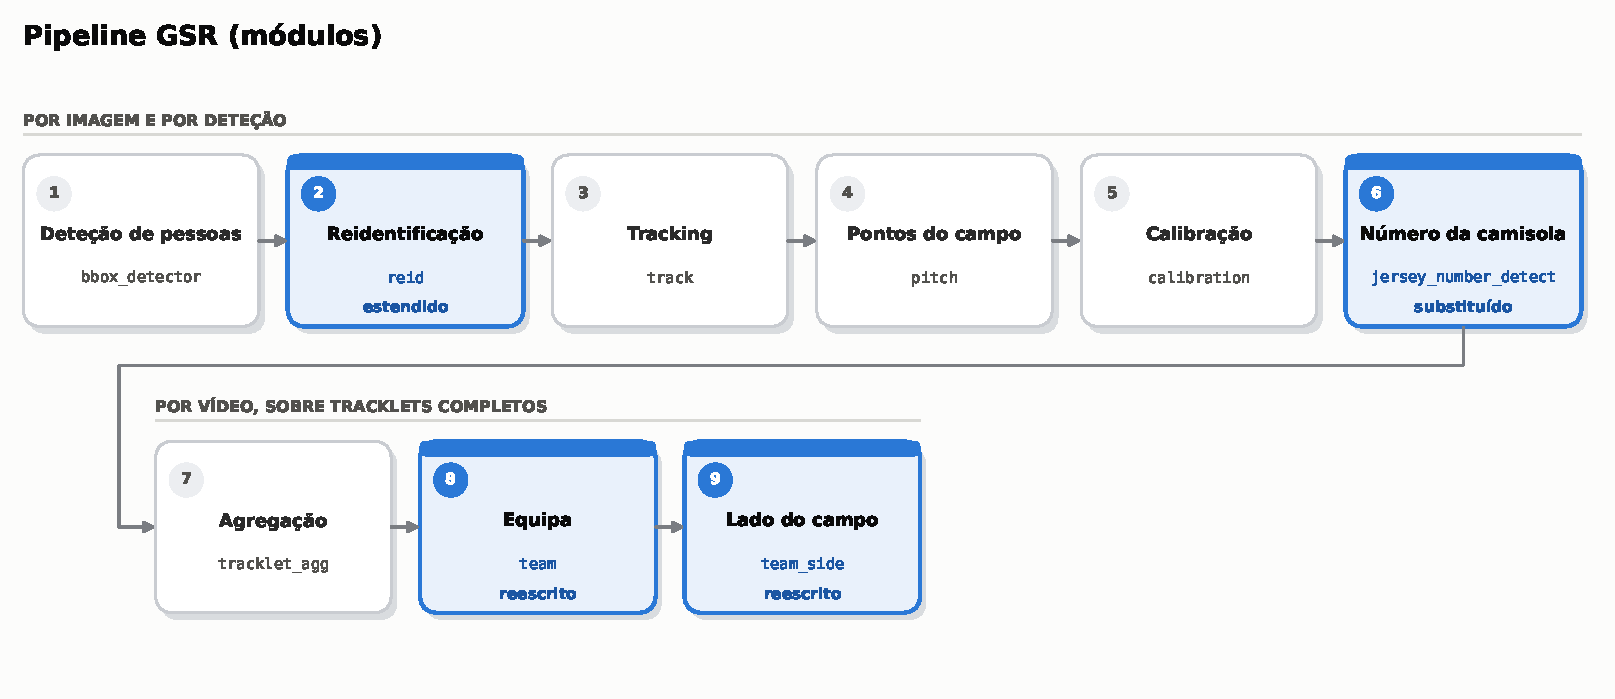
\includegraphics[width=\textwidth]{fig_pipeline_modulos.pdf}
    \caption{Os nove módulos do \emph{pipeline} da \emph{baseline}, pela ordem em que são executados. A azul, os quatro módulos em que este trabalho intervém. A reidentificação foi estendida com um descritor de cor, sem alterar o modelo nem o vetor de aparência original. O reconhecimento do número da camisola passou a ser feito por um módulo novo. O agrupamento em equipas e a atribuição do lado do campo foram reescritos. Os restantes cinco módulos correm com o código e os pesos originais.}
    \label{fig:pipeline-modulos}
\end{figure}

Este trabalho intervém em quatro dos nove módulos, assinalados a azul na Figura~\ref{fig:pipeline-modulos}. No reconhecimento do número da camisola (módulo 6), o MMOCR da \emph{baseline}, que lê cada recorte isoladamente, dá lugar a um modelo multimodal de visão e linguagem, descrito na Secção~\ref{sec:met-jnr}. O módulo continua a ser de nível deteção, mas guarda os recortes de cada \emph{tracklet} e só decide o número no fim do vídeo, quando o \emph{tracklet} está completo, o que lhe permite escolher as leituras em que confia. Os módulos da equipa e do lado do campo (módulos 8 e 9) são reescritos. O agrupamento passa a ser auditado e o lado passa a ser decidido por uma cascata de critérios, descritos na Secção~\ref{sec:met-equipa}. A reidentificação (módulo 2) é estendida sem ser alterada. O modelo e o vetor de aparência que o \emph{tracking} usa mantêm-se intactos, e acrescenta-se, para cada deteção, um descritor da cor do equipamento, que o módulo da equipa usa quando o vetor de aparência não chega para separar as equipas. Os restantes cinco módulos, a deteção, o \emph{tracking}, os pontos do campo, a calibração e a agregação, correm com o código e os pesos originais.

Os módulos alterados correspondem às lacunas identificadas na Secção~\ref{sec:sintese_lacunas}. O número da camisola é o atributo que mais custa ao GS-HOTA, tanto na \emph{baseline} como nos melhores sistemas do desafio. Entre os atributos de identificação, a equipa vem logo a seguir. O lado do campo, por sua vez, nunca tinha sido medido com \emph{tracklets} reais. Manter intactos os outros cinco garante que qualquer diferença de desempenho resulta das alterações introduzidas, e não de uma reotimização global do \emph{pipeline}. Como nenhuma das alterações exige treinar modelos, todas se integram na \emph{baseline} pública de \citet{somers2024soccernet} sem voltar a treinar as etapas anteriores.



\section{Reconhecimento do Número da Camisola}\label{sec:met-jnr}

Na \emph{baseline}, o reconhecimento do número da camisola é feito pela biblioteca MMOCR, que aplica um \emph{pipeline} genérico de deteção e reconhecimento de texto ao recorte do corpo inteiro de cada jogador. Como procura texto em todo o recorte, sem qualquer conhecimento prévio do domínio, esta abordagem trata o número como um texto qualquer e ignora duas propriedades do problema.

A primeira é espacial. O número encontra-se numa região anatomicamente delimitada, a zona dorsal do tronco, cuja localização pode ser estimada com precisão por um modelo de pose, em vez de ser procurada em todo o recorte. A segunda é temporal. O mesmo jogador é visto em muitas imagens consecutivas, mas o número só é legível em parte delas, por causa da baixa resolução, das oclusões e das poses desfavoráveis. Na \emph{baseline}, as leituras de todas as imagens são combinadas por votação simples, em que uma leitura nítida e uma leitura adivinhada valem o mesmo. Tirar partido desta redundância exige distinguir umas das outras.

Para aproveitar estas duas propriedades, o módulo proposto organiza o reconhecimento em três fases (Figura~\ref{fig:jnr-flow}). Primeiro, um modelo de estimativa de pose, o YOLO26m-pose \citep{jocher2026yolo26}, localiza os pontos do tronco (\emph{keypoints}) e isola a região dorsal, eliminando o fundo e as áreas irrelevantes do recorte. Depois, essa região é lida por um modelo multimodal de visão e linguagem (\emph{Vision-Language Model}, VLM), o Qwen2.5-VL \citep{bai2025qwen25vl}. O modelo interpreta a imagem no contexto do equipamento e distingue o número de outros elementos gráficos, como os patrocínios. Por fim, as leituras de cada \emph{tracklet} são combinadas numa decisão única, na qual só contam as leituras em que o próprio modelo indica estar seguro. As subsecções seguintes descrevem cada fase e justificam a escolha de cada modelo.


\begin{figure}[htbp]
    \centering
    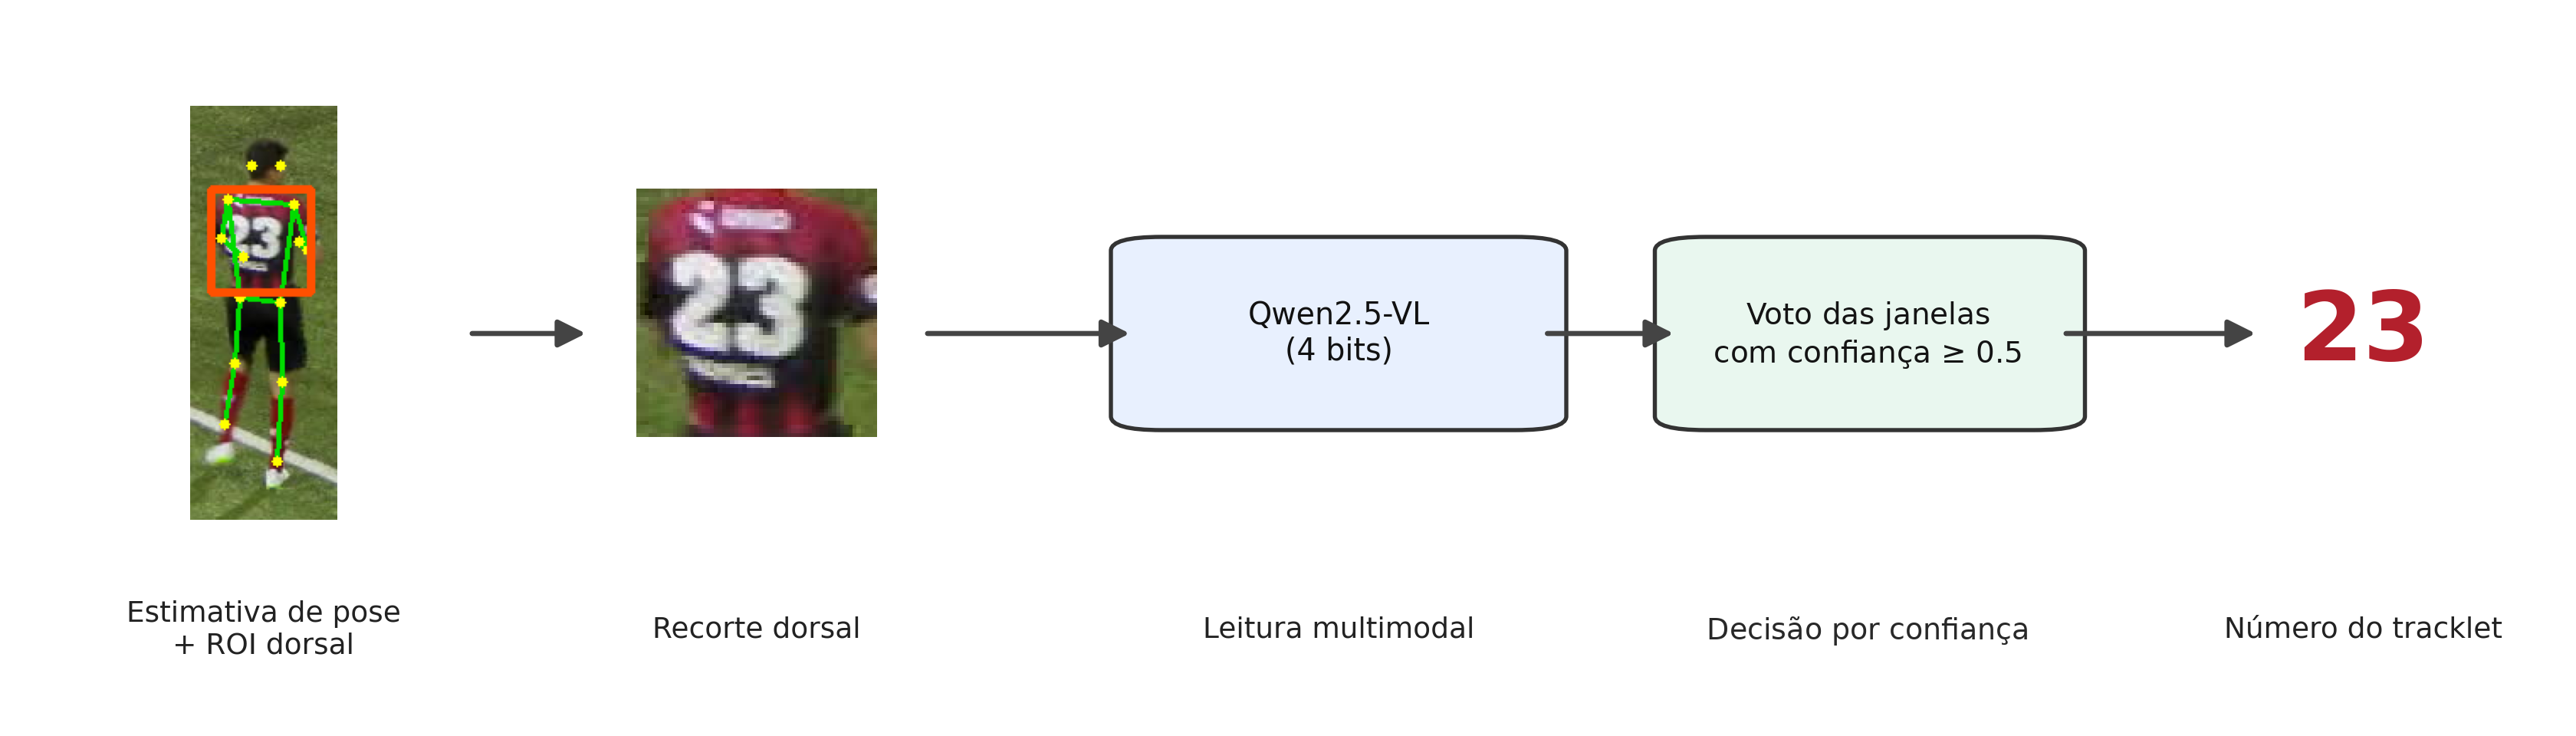
\includegraphics[width=\textwidth]{jnr_flow.png}
    \caption{Fluxo do módulo de reconhecimento do número da camisola. A estimativa de pose delimita a região dorsal, cujo recorte é interpretado pelo modelo multimodal Qwen2.5-VL quantizado a 4 bits. As leituras sucessivas de cada \emph{tracklet} são combinadas numa decisão final única, contando apenas as leituras com confiança suficiente.}
    \label{fig:jnr-flow}
\end{figure}

\subsection{Recorte da Região Dorsal por Estimativa de Pose}

Para concentrar a leitura na zona onde o número efetivamente aparece, cada deteção é primeiro processada por um modelo de estimativa de pose, o YOLO26m-pose. Usou-se a geração mais recente da família YOLO à data do trabalho, que sucedeu ao YOLOv11-pose das primeiras versões do módulo, na sua variante média, como compromisso entre a qualidade dos \emph{keypoints} e o tempo de execução, uma vez que o modelo corre sobre todas as deteções do vídeo. A partir dos \emph{keypoints} dos ombros e das ancas, define-se uma região de interesse sobre as costas do jogador, alargada lateralmente para acomodar variações de postura e enquadramento. O recorte é rejeitado quando o nariz ou um dos olhos é detetado com confiança superior a $0.6$, sinal de que o jogador está de frente para a câmara, ou quando os ombros e as ancas não são detetados com confiança suficiente. Esta regra simples foi a única filtragem da orientação que se manteve, depois de um classificador de orientação mais elaborado ter sido testado e descartado (Tabela~\ref{tab:alternativas}). O recorte final entrega ao modelo de leitura apenas a zona das costas, sem o fundo, os membros e a parte da frente.

Antes da leitura, cada recorte passa por um filtro de qualidade. São rejeitados os recortes com menos de $15\times20$ píxeis, tipicamente de jogadores muito distantes da câmara, e os recortes desfocados, cuja nitidez, medida pela variância do Laplaciano, fica abaixo de $15$. Estes limiares são baixos de propósito, para que o filtro elimine apenas os recortes claramente ilegíveis. Numa primeira versão do módulo, o filtro era a única defesa contra leituras de recortes sem informação, e os limiares tinham de ser altos ($25\times30$ píxeis e nitidez de $40$), o que excluía também jogadores cujo número era legível. Com a decisão pela confiança da leitura (Secção~\ref{sec:met-jnr-confianca}), é o próprio modelo que indica quando não conseguiu ler, e o filtro passa a servir apenas para evitar chamadas inúteis ao modelo.


\subsection{Leitura por Modelo Multimodal de Visão e Linguagem}

A leitura do número é feita pelo Qwen2.5-VL-3B-Instruct, um modelo multimodal de visão e linguagem (\emph{Vision-Language Model}, VLM) que recebe os recortes da região dorsal e devolve o número em texto. Preferiu-se um VLM a um motor de OCR dedicado porque o VLM interpreta o recorte no seu contexto. Distingue assim o número do jogador de outros elementos gráficos do equipamento, como patrocínios, logótipos ou textos avulsos, que um motor de OCR leria como texto e que introduziriam erros.

A principal restrição prática foi a memória da GPU, uma NVIDIA RTX~3060 portátil com 6~GB de VRAM partilhados com os restantes módulos. Em 16 bits, a precisão em que é distribuído, o Qwen2.5-VL-3B ocupa cerca de 7~GB e não cabe na GPU. Foi por isso carregado com quantização a 4 bits, através da biblioteca \emph{bitsandbytes}.

Quantizar um modelo é representar os seus pesos com menos bits do que os usados no treino, em troca de um pequeno erro de arredondamento \citep{gholami2021survey}. A \emph{bitsandbytes} fá-lo por blocos \citep{dettmers2023case, dettmers2023qlora}. Os pesos de cada camada linear são divididos em blocos de 64, e cada bloco é dividido pelo seu maior valor absoluto, que fica guardado em 32 bits como escala. Cada peso normalizado, agora entre $-1$ e $1$, é arredondado para o valor mais próximo do formato FP4, um número de vírgula flutuante de 4 bits, e é esse código de 4 bits que se guarda. Num bloco do próprio modelo, com escala $0.0510$, o peso $-0.0427$ dá $-0.837$ e fica guardado como $-1$. No cálculo, o código é multiplicado pela escala e convertido de novo para 16 bits. Cada peso passa a custar 4.5 bits em vez de 16, sem dados de calibração nem novo treino.

No Qwen2.5-VL-3B, as 414 camadas lineares são quantizadas no carregamento, com a configuração por omissão da biblioteca. Só a camada final, que produz as pontuações de cada \emph{token} usadas na Secção~\ref{sec:met-jnr-confianca}, fica em 16 bits. O modelo passa a ocupar 2.4~GB na GPU. O efeito da quantização na exatidão da leitura não foi medido, porque o modelo em 16 bits não cabe na GPU disponível.

O modelo é ainda libertado da GPU no fim de cada vídeo e recarregado no início do seguinte, para que os modelos dos pontos do campo e da calibração do vídeo seguinte, que correm antes do reconhecimento do número, não fiquem sem memória.

O \emph{prompt} dá ao modelo duas instruções. A primeira é ler o número inteiro. Sem ela, o modelo omite com frequência o primeiro algarismo quando este está parcialmente tapado, e lê, por exemplo, um 14 como 4. A segunda é não responder quando o recorte está pouco nítido, desfocado ou ambíguo, em vez de arriscar uma leitura incerta.

A política de recusa decorre da métrica. No GS-HOTA, um número errado nunca custa menos do que a ausência de resposta. Quando o jogador tem número anotado, os dois contam como erro. Quando não tem, só o número inventado é penalizado. É por isso preferível que o modelo não responda a que arrisque uma leitura incerta (Secção~\ref{sec:met-jnr-confianca}).

Para reduzir o número de chamadas ao modelo, a leitura feita durante a execução do \emph{pipeline} agrupa vários \emph{tracklets} na mesma chamada. Cada \emph{tracklet} entra como um grupo de recortes, identificado por um rótulo, e o modelo responde com uma linha por grupo, com o número ou com a indicação de que não o consegue ler. Cada chamada leva no máximo quatro \emph{tracklets} e vinte recortes, os mais nítidos de cada um. Este limite resultou de ensaios durante o desenvolvimento, nos quais a qualidade das respostas caía quando o modelo recebia mais de 15 a 20 imagens de uma vez. Os primeiros recortes de cada \emph{tracklet} são lidos numa chamada à parte. Juntá-los nessa fase a imagens de qualidade muito diferente levava o modelo a recusar a leitura de todos os grupos, mesmo dos que tinham o número visível. A leitura usada na decisão final é feita à parte, sobre conjuntos de recortes consecutivos, as janelas descritas na secção seguinte.

\subsection{Confiança da Leitura e Decisão por Janela}\label{sec:met-jnr-confianca}

A leitura efetuada sobre um recorte isolado é, por natureza, ruidosa. Uma pose desfavorável, uma oclusão momentânea ou variações de iluminação bastam para levar a uma leitura errada num \emph{frame}, mesmo quando o número se mantém legível na maior parte do \emph{tracklet} (Figura~\ref{fig:jnr-crops}). A decisão final tem, por isso, de combinar várias leituras, e a forma de as combinar determina o tipo de erro que o sistema comete.

\begin{figure}[H]
    \centering
    
\includegraphics[width=0.9\textwidth]{jnr_crops_tracklet71.png}
    \caption{Recortes da região dorsal de um mesmo \emph{tracklet} ao longo do tempo. O número do jogador é nítido apenas em parte dos \emph{frames}. Esta variabilidade justifica decidir o número apenas com as leituras em que o modelo indica estar seguro.}
    \label{fig:jnr-crops}
\end{figure}

Para cada \emph{tracklet}, os recortes da região dorsal que passam o filtro de qualidade são ordenados no tempo e agrupados em janelas de seis recortes consecutivos, e cada janela dá origem a uma leitura (Figura~\ref{fig:jnr-janelas}). Para essa leitura escolhem-se os cinco recortes mais nítidos da janela, medidos pela variância do Laplaciano, que são apresentados em conjunto ao Qwen2.5-VL numa única chamada, com o \emph{prompt} descrito na secção anterior. A resposta é gerada com descodificação determinística (\emph{greedy decoding}), em que o modelo escreve, em cada passo, o \emph{token} mais provável, sem amostragem aleatória, pelo que a mesma janela produz sempre a mesma resposta. O modelo responde com um número ou recusa a leitura.

A confiança da leitura obtém-se da própria resposta. O Qwen2.5-VL escreve os números um dígito de cada vez, e cada dígito é um \emph{token} ao qual o modelo atribui uma probabilidade que mede a sua segurança. A confiança da janela é o produto das probabilidades dos dígitos do número. Para o número 14 lido com probabilidade $0.97$ no primeiro dígito e $0.93$ no segundo, a confiança é $0.97 \times 0.93 \approx 0.90$. Existe, assim, uma única confiança por janela, calculada sobre a resposta e não sobre cada recorte. Um número lido com segurança tem confiança próxima de $1$, enquanto um número adivinhado num recorte pouco legível fica muito abaixo, porque basta a incerteza num dos dígitos para baixar o produto.

\begin{figure}[H]
    \centering
    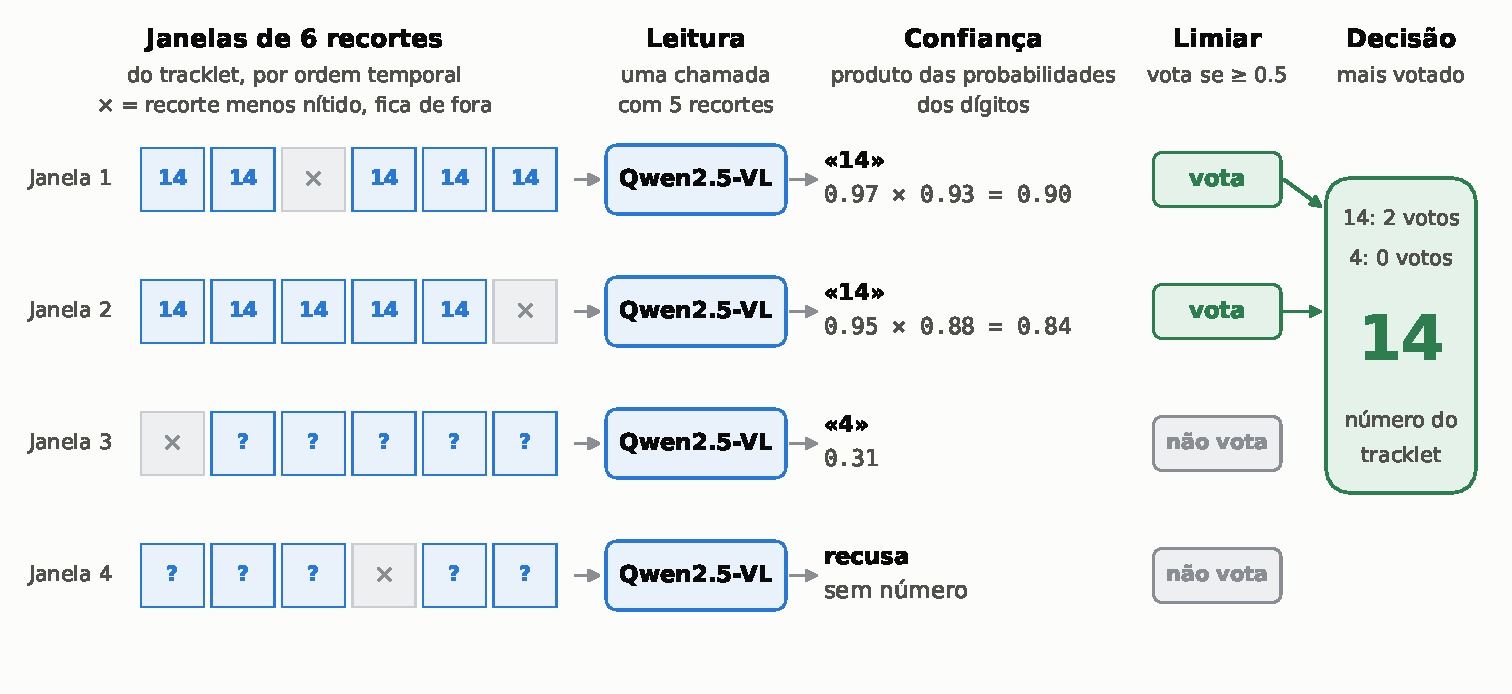
\includegraphics[width=\textwidth]{fig_jnr_janelas.pdf}
    \caption{Decisão do número de um \emph{tracklet} por janelas. Os recortes são agrupados em janelas de seis, e os cinco mais nítidos de cada janela são lidos numa única chamada ao Qwen2.5-VL. Nas janelas 3 e 4, o «?» marca os recortes em que o número não se lê. A confiança de cada leitura é o produto das probabilidades dos seus dígitos. Só votam as janelas com confiança igual ou superior a $0.5$, e o \emph{tracklet} recebe o número mais votado.}
    \label{fig:jnr-janelas}
\end{figure}

No fim do \emph{tracklet}, as leituras de todas as janelas são combinadas por votação, com duas regras. Uma janela só vota se tiver lido um número com confiança igual ou superior a $0.5$, pelo que não votam as janelas com confiança inferior nem aquelas em que o modelo recusou a leitura. O \emph{tracklet} recebe o número mais votado entre as janelas que votaram e, se nenhuma votou, fica sem número. A confiança decide, assim, que leituras contam, e a maioria decide o número.

Esta regra resulta de um diagnóstico realizado no próprio módulo. Na primeira versão, a função que chamava o modelo devolvia sempre a mesma confiança fixa, independentemente da certeza da leitura, e a decisão dependia apenas da contagem de votos, com uma quota mínima de concordância entre as janelas. Um número nítido e um número adivinhado, num recorte desfocado, pesavam o mesmo. Quando um jogador era visto durante muito tempo em más condições, as leituras erradas acumulavam votos suficientes para vencer, e o erro propagava-se a centenas de deteções. A confiança do modelo já existia, mas era descartada. Usá-la permite separar as leituras seguras das restantes antes da votação, em vez de tentar compensar a posteriori com quotas de concordância.

O limiar de 0.5 traduz uma escolha de projeto. Na métrica do SoccerNet-GSR, errar o número nunca custa menos do que deixá-lo em branco, e é pior quando o jogador não o tem anotado. Fora da métrica, a diferença é ainda maior. Um número errado dá ao jogador a identidade de outro, e a ausência de resposta apenas a deixa por atribuir. Entre errar e abster-se, o sistema foi desenhado para se abster. O custo desta escolha, medido no Capítulo~\ref{cap:resultados}, é um ligeiro aumento dos jogadores que ficam sem número.


\subsection{Alternativas Consideradas}

A solução final para a leitura do número não foi imediata. Antes de se chegar ao Qwen2.5-VL-3B, testaram-se abordagens de quatro tipos. O primeiro foi o de outros motores de OCR, como o EasyOCR \citep{jaidedai2020easyocr}, o PaddleOCR \citep{li2022ppocrv3} e o HunyuanOCR \citep{hunyuan2025ocr}. O segundo foi a versão maior do mesmo modelo, o Qwen2.5-VL-7B, com 7 mil milhões de parâmetros em vez de 3 mil milhões. O terceiro foi ampliar os recortes por super-resolução, com o Real-ESRGAN \citep{wang2021realesrgan}, antes de os ler. O quarto foram duas formas de pôr de parte os recortes em que o jogador não está de costas. Uma usava a reconstrução tridimensional do corpo pelo SAM 3D Body \citep{yang2026sam3dbody}, e a outra um classificador de orientação.

\begin{table}[htbp]
\centering
\caption{Alternativas consideradas para a leitura do número e motivo por que foram postas de parte.}
\label{tab:alternativas}
\renewcommand{\arraystretch}{1.35}
\setlength{\tabcolsep}{6pt}
\begin{tabular}{|p{3.6cm}|p{9.0cm}|}
\hline
\textbf{Abordagem} & \textbf{Razão do descarte} \\
\hline
EasyOCR e OCR clássico &
Mesma limitação estrutural do MMOCR, falha em números pequenos ou inclinados e não
distingue o número de outros elementos gráficos. \\
\hline
PaddleOCR (com \emph{fine-tuning}) &
Falha de segmentação (\emph{segfault}) ao inicializar no mesmo processo que o CUDA do
\emph{pipeline}, e mesmo isolado não recuperou leituras face ao Qwen. \\
\hline
HunyuanOCR &
\emph{VLM} mais pesado, sem ganho de exatidão que compensasse o custo de VRAM e de
latência no \emph{hardware} disponível. \\
\hline
Qwen2.5-VL-7B &
Requer cerca de 10\,GB de VRAM, acima dos 6\,GB da GPU, o que inviabiliza a sua
utilização. \\
\hline
Super-resolução (\mbox{Real-ESRGAN}) &
A informação em falta não existe na imagem de origem, e a ampliação amplifica o ruído
em vez de a recuperar. \\
\hline
SAM 3D Body &
Reconstrução tridimensional do corpo demasiado pesada para correr por \emph{frame} e
desadequada a um simples sinal de orientação. \\
\hline
Classificador de orientação &
O ganho de filtrar os \emph{frames} sem as costas visíveis não compensou, pois a votação
por \emph{tracklet} já absorve naturalmente esses \emph{frames}. \\
\hline
\end{tabular}
\end{table}


Estas experiências convergem numa conclusão. Em condições de baixa resolução, o fator decisivo não é a escolha do motor de OCR mais potente, mas sim entregar ao modelo a imagem certa, o recorte da região dorsal obtido por pose, e agregar bem as leituras ao longo do tempo. O Qwen2.5-VL-3B foi escolhido pelo equilíbrio entre exatidão e ocupação de memória, e não por ser o modelo de maior dimensão.


\section{Atribuição da Equipa e do Lado do Campo}\label{sec:met-equipa}

A atribuição da equipa divide-se em dois problemas distintos. O primeiro consiste em separar os \emph{tracklets} dos jogadores em dois grupos, um por equipa. O segundo consiste em determinar qual dos grupos defende a baliza da esquerda e qual defende a da direita. Este segundo passo é necessário porque a anotação do SoccerNet-GSR identifica as equipas pelo lado do campo que defendem, \emph{left} ou \emph{right}, e não pelo nome ou pela cor do equipamento. Um erro em qualquer dos dois problemas conta como erro na atribuição da equipa.

A \emph{baseline} resolve os dois problemas de forma simples. No primeiro, calcula para cada \emph{tracklet} de jogador a média das suas características de reidentificação, um vetor de 256 dimensões produzido pelo PRTreID, e agrupa esses vetores com um \emph{k-means} de dois grupos. O \emph{k-means} é um algoritmo de agrupamento não supervisionado que reparte as observações num número fixo de grupos. Cada observação é atribuída ao centro mais próximo e os centros são recalculados até a partição estabilizar. No segundo problema, a solução calcula a média da coordenada horizontal no campo de todas as deteções de cada grupo e declara \emph{right} o grupo com a média mais à direita. Os guarda-redes ficam fora do agrupamento e recebem, em cada deteção, o lado correspondente à metade do campo em que se encontram. Nenhum destes resultados é auditado. Se o \emph{k-means} misturar as equipas, os \emph{tracklets} mal agrupados ficam com a equipa errada. Se a média das posições apontar para o lado errado, todos os jogadores do vídeo ficam com o lado trocado.

Foi isso que a inspeção visual da \emph{baseline} mostrou, como o Capítulo~\ref{cap:resultados} quantifica. Nos $159$ vídeos, as falhas do próprio módulo de equipa repartem-se entre o agrupamento, com $14$ vídeos de equipas misturadas e $7$ colapsados numa só equipa, e o mapeamento para os lados, com $7$ vídeos de lado trocado. O lado trocado é a falha mais grave, porque deixa a $0\%$ todos os \emph{tracklets} do vídeo, mesmo quando os dois grupos estão corretos. Outros $20$ vídeos falham antes do agrupamento, no classificador de função, que este trabalho não alterou. As alterações descritas a seguir atuam por isso nas duas fases do processo, mas de forma diferente. No agrupamento, mantém-se o método original e acrescenta-se uma auditoria que, quando o resultado é pouco fiável, recorre a um agrupamento alternativo pela cor do equipamento. Esta alternativa exige um descritor novo, calculado no módulo de reidentificação. No mapeamento para os lados, substitui-se a comparação de médias por uma cascata de quatro critérios, em que essa comparação passa a ser o último recurso.

\subsection{Descritor de Cor do Equipamento}\label{sec:descritor-cor}

Para separar as equipas, a \emph{baseline} usa o vetor de $256$ números com que o PRTreID descreve a aparência de cada jogador. Este vetor foi treinado sobretudo para reconhecer o mesmo jogador ao longo do vídeo, e não para agrupar os jogadores por equipa. Por isso mistura a cor do equipamento com outros traços, como a forma do corpo, a pose ou o cabelo. Quando os equipamentos das duas equipas são parecidos, ou quando a imagem é pequena ou mal iluminada, dois jogadores de equipas diferentes podem ficar tão próximos como dois jogadores da mesma equipa, e o agrupamento mistura as equipas.

Para dispor de um sinal que dependa apenas da cor da camisola, acrescentou-se ao módulo de reidentificação um descritor de cor, calculado para cada deteção. O descritor tem $27$ números e é construído em três passos, ilustrados na Figura~\ref{fig:descritor-cor}. Primeiro, isolam-se os píxeis da camisola. Depois, descreve-se a cor desses píxeis. Por fim, guarda-se o resultado ao lado do vetor original, sem o alterar.

\begin{figure}[H]
    \centering
    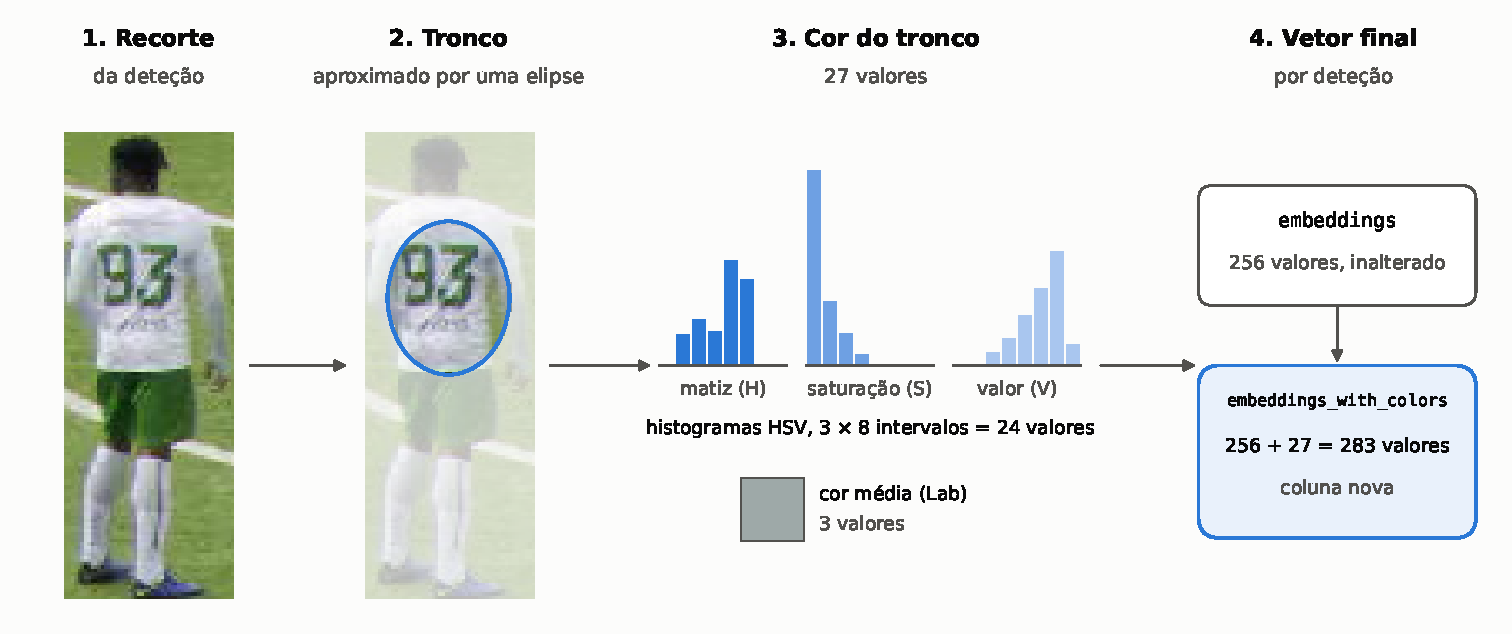
\includegraphics[width=\textwidth]{fig_descritor_cor.pdf}
    \caption{Construção do descritor de cor para uma deteção do vídeo SNGS-116, do recorte da deteção ao vetor final guardado na coluna nova.}
    \label{fig:descritor-cor}
\end{figure}

Para isolar a camisola aproveita-se um resultado que o PRTreID já calcula. O modelo divide o corpo em seis partes, a cabeça, o tronco, os dois braços e as duas pernas, e produz para cada deteção um mapa que indica onde está cada parte. Usam-se apenas os píxeis em que o mapa do tronco atinge pelo menos $25\%$ do seu valor máximo, o que deixa de fora a relva, a pele, os calções e as meias. Nas deteções muito pequenas ou cortadas, em que o tronco reúne menos de $16$ píxeis, usa-se em alternativa a faixa central do recorte, entre $25\%$ e $75\%$ da altura. Como o mapa não é guardado, a Figura~\ref{fig:descritor-cor} representa o tronco por uma elipse.

A cor dos píxeis do tronco é descrita no espaço HSV, que representa cada píxel por três valores. A matiz indica a cor propriamente dita, como o vermelho ou o azul. A saturação indica se a cor é viva ou acinzentada, e o valor se é clara ou escura. São estes dois últimos canais que distinguem os equipamentos brancos, pretos ou cinzentos, que não têm matiz definida. Para cada canal, a escala de valores possíveis é dividida em oito intervalos iguais, cada píxel da camisola cai num desses intervalos e conta-se a fração dos píxeis que cai em cada um. Os três canais dão assim $3 \times 8 = 24$ números, que a Tabela~\ref{tab:hsv-exemplo} mostra para a camisola branca da Figura~\ref{fig:descritor-cor}. Saturação baixa e valor alto é o que caracteriza uma camisola branca. Juntam-se mais três números, a cor média dos mesmos píxeis no espaço Lab, um espaço em que a distância entre duas cores acompanha a diferença que o olho humano percebe.

\begin{table}[H]
    \centering
    \definecolor{azultab}{HTML}{2A78D6}
    \caption{Histograma HSV da camisola da Figura~\ref{fig:descritor-cor}, calculado sobre os $1336$ píxeis do tronco. Cada valor é a fração dos píxeis que cai em cada intervalo, do mais baixo ($1$) ao mais alto ($8$). Quanto mais escura a célula, maior a fração.}
    \label{tab:hsv-exemplo}
    \small
    \setlength{\tabcolsep}{4pt}
    \begin{tabular}{|l|c|c|c|c|c|c|c|c|l|}
        \hline
        \textbf{Canal} & \textbf{1} & \textbf{2} & \textbf{3} & \textbf{4} & \textbf{5} & \textbf{6} & \textbf{7} & \textbf{8} & \textbf{Leitura} \\
        \hline
        Matiz (H) & $0.00$ & \cellcolor{azultab!9}$0.10$ & \cellcolor{azultab!13}$0.15$ & \cellcolor{azultab!9}$0.11$ & \cellcolor{azultab!30}$0.35$ & \cellcolor{azultab!24}$0.28$ & $0.00$ & $0.00$ & Pouco fiável no branco \\
        \hline
        Saturação (S) & \cellcolor{azultab!55}$0.64$ & \cellcolor{azultab!18}$0.21$ & \cellcolor{azultab!9}$0.11$ & \cellcolor{azultab!3}$0.04$ & $0.00$ & $0.00$ & $0.00$ & $0.00$ & Baixa, sem cor viva \\
        \hline
        Valor (V) & $0.00$ & $0.00$ & \cellcolor{azultab!3}$0.04$ & \cellcolor{azultab!8}$0.09$ & \cellcolor{azultab!15}$0.17$ & \cellcolor{azultab!22}$0.26$ & \cellcolor{azultab!33}$0.38$ & \cellcolor{azultab!6}$0.07$ & Alto, cor clara \\
        \hline
    \end{tabular}
\end{table}

Os $27$ números são acrescentados aos $256$ do PRTreID e guardados numa coluna nova, \texttt{embeddings\_\allowbreak with\_\allowbreak colors}, com $283$ valores. A coluna original, \texttt{embeddings}, fica igual, e por isso o \emph{tracking}, que a usa, funciona exatamente como na \emph{baseline}. Só o agrupamento em equipas lê a coluna nova, e dela usa apenas os $27$ números de cor. Os casos em que o agrupamento recorre a estes números são descritos na Secção~\ref{sec:agrupamento}, e o efeito no resultado é medido na Secção~\ref{sec:res_equipa_ablacao}.

\subsection{Agrupamento em Duas Equipas com Auditoria}\label{sec:agrupamento}

O \emph{k-means} divide os \emph{tracklets} de jogador em dois grupos, um por equipa, e é a esta divisão que se chama agrupamento. Devolve sempre dois grupos, mesmo quando as características que recebe não separam as equipas, e a \emph{baseline} aceita o resultado sem o verificar. O módulo reescrito parte do mesmo agrupamento, mas submete-o a duas verificações antes de o aceitar. A primeira, «Separação clara?», verifica se os dois grupos estão bem separados no espaço de reidentificação. Se não estiverem, o agrupamento é refeito com o descritor de cor da Secção~\ref{sec:descritor-cor}, e o novo agrupamento só é usado se passar a verificação «Cor aceite?». A segunda, «Duas equipas?», verifica se o agrupamento que sai da primeira tem, de facto, duas equipas. Se não tiver, os \emph{tracklets} são reagrupados pela cor medida diretamente nas imagens, e este agrupamento de resgate só é usado se passar a verificação «Resgate aceite?». Sempre que uma alternativa é recusada, mantém-se o agrupamento que vinha de trás. Quando nenhuma verificação falha, o agrupamento final é o da reidentificação, como na \emph{baseline}.

O primeiro passo é o da \emph{baseline}. Para cada \emph{tracklet} de jogador calcula-se a média de três grandezas ao longo das suas deteções, o vetor de reidentificação de $256$ números, o descritor de cor de $27$ números e a posição horizontal no campo. Esta posição é a coordenada $x$ dos pés do jogador no mapa do campo, que a calibração exprime em metros, com origem no centro. Como o campo do SoccerNet-GSR tem $105$ metros de comprimento, $x$ vai de $-52.5$ metros, na linha de baliza da esquerda, a $+52.5$ metros, na da direita. Uma deteção com $|x|$ acima de $52.5$ metros fica para lá da linha de baliza, o que num jogador em campo resulta quase sempre de uma falha pontual da calibração, capaz de projetar os pés a centenas de metros. Essas deteções são ignoradas, porque uma só bastaria para deslocar a média do \emph{tracklet}, e a média só é calculada se restarem pelo menos três deteções. Os vetores de reidentificação são então agrupados com um \emph{k-means} de dois grupos, que corre dez vezes com centros iniciais diferentes e fica com o resultado mais compacto, para que não dependa de um mau ponto de partida. A cor e a posição ainda não entram nesta fase e só são usadas nas verificações descritas a seguir, a posição para saber em que metade do campo está cada \emph{tracklet}. A reidentificação é, portanto, o sinal principal. Na maioria dos vídeos é ela que separa as equipas, e a cor só é chamada quando essa separação não é fiável.


A decisão «Separação clara?» usa duas medidas. A primeira é o coeficiente de silhueta. Para cada \emph{tracklet}, compara-se a distância média aos \emph{tracklets} do seu grupo com a distância média aos do outro grupo, o que dá um valor entre $-1$ e $1$. Perto de $1$, os grupos são compactos e afastados, como se espera de duas equipas com equipamentos diferentes. Perto de zero, sobrepõem-se e a divisão pode ser arbitrária. A segunda medida é a distância entre os centros dos dois grupos no espaço de reidentificação. A separação é dada como pouco clara em dois casos. No primeiro, a silhueta média fica abaixo de $0.28$. No segundo, herdado de uma versão anterior do módulo, pelo menos $85\%$ dos \emph{tracklets} estão na mesma metade do campo e os centros distam menos de $2.04$. Nesses vídeos a posição dos jogadores pouco ajuda a decidir o lado, e um erro de agrupamento sai mais caro.

O valor de $2.04$ não tem significado geral e deve ser lido como tal. Nos quatro vídeos de teste em que o segundo caso se verifica, a distância entre centros foi de $1.799$, $1.896$, $1.981$ e $2.035$, e o limiar ficou $0.005$ acima do maior destes valores. Manteve-se porque retirá-lo introduzia regressões no conjunto de teste. O primeiro caso foi acrescentado mais tarde, calibrado sobre os conjuntos de teste e de validação em conjunto, precisamente para cobrir os vídeos em que a jogada não se concentra numa metade e o segundo caso nunca se verifica.

Quando a separação não é clara, o \emph{k-means} é repetido sobre os $27$ números do descritor de cor, normalizados para que cada um tenha média zero e desvio-padrão um. A cor é usada sozinha, e não junta aos $256$ números da reidentificação, porque depois da normalização todos os números pesam o mesmo e os $256$ da reidentificação abafariam os $27$ da cor. A decisão «Cor aceite?» exige que o grupo menor do agrupamento por cor reúna pelo menos $20\%$ dos \emph{tracklets}. Abaixo disso, o \emph{k-means} terá isolado um punhado de \emph{tracklets} atípicos, com sombra ou oclusão, e não as duas equipas, e mantém-se o agrupamento por reidentificação. Esta exigência só se aplica ao primeiro caso. No segundo, o agrupamento por cor é sempre aceite, para manter o comportamento já validado da versão anterior. A Figura~\ref{fig:team_cluster} mostra, para um vídeo real, os dois espaços em que o agrupamento é feito.

\begin{figure}[H]
    \centering
    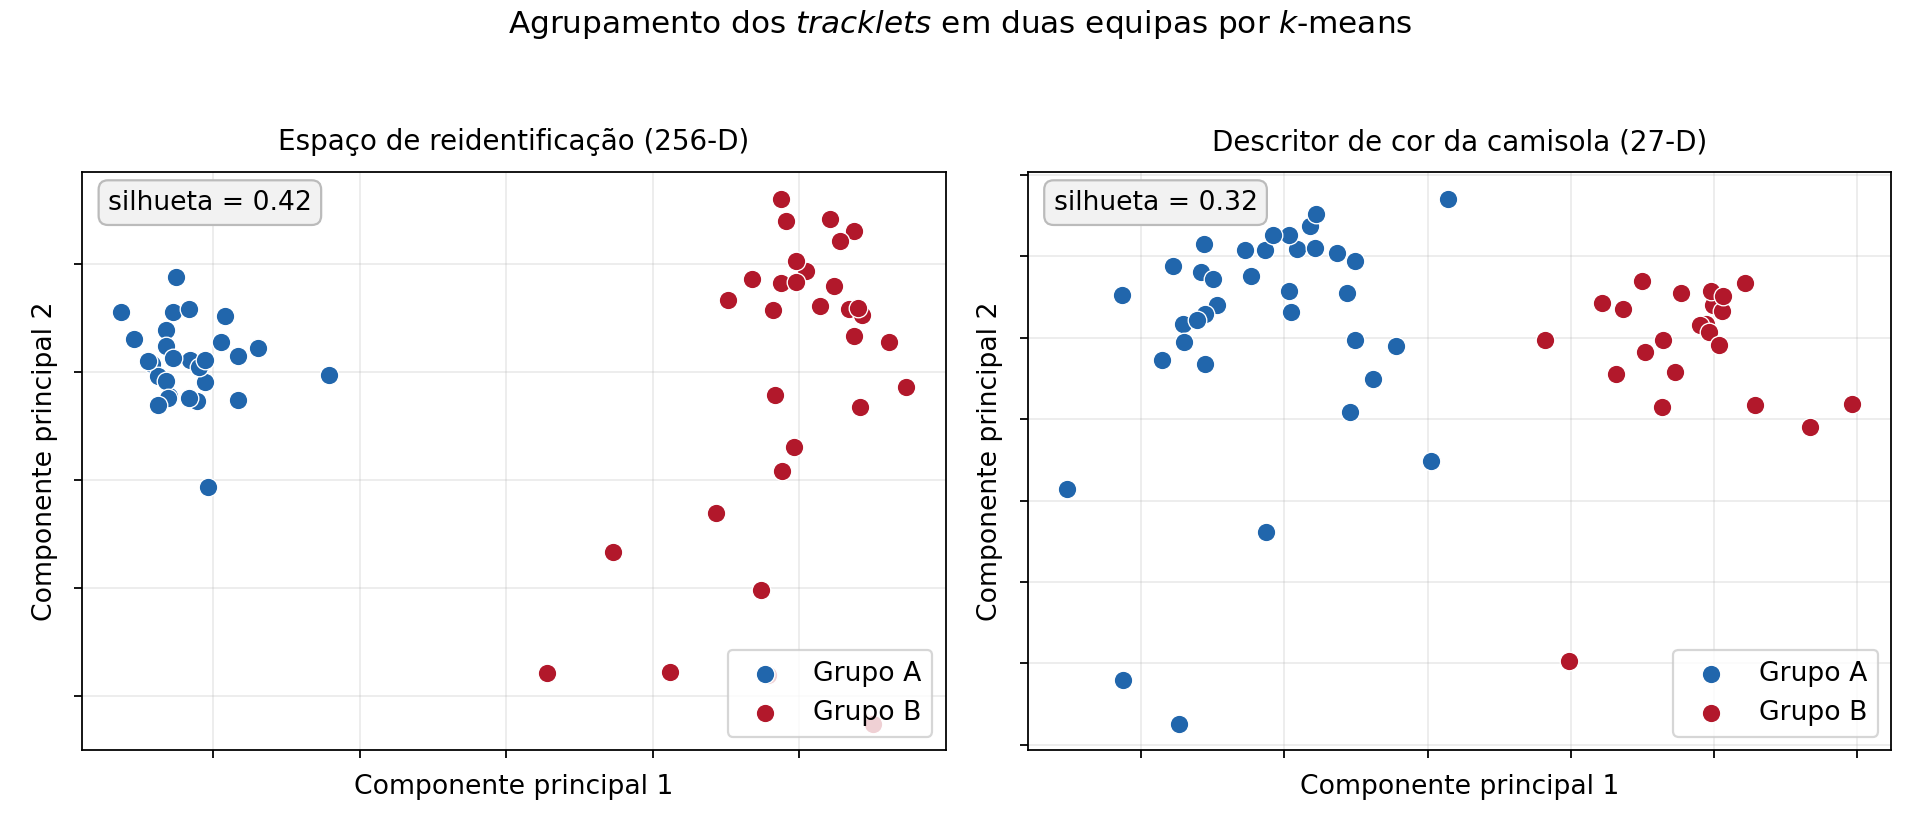
\includegraphics[width=\textwidth]{team_cluster_space.png}
    \caption{Agrupamento dos \emph{tracklets} de um vídeo nas duas equipas. À esquerda, a projeção das características de reidentificação em duas dimensões, onde o \emph{k-means} separa os dois grupos com um coeficiente de silhueta de $0.42$. À direita, o descritor de cor da camisola dos mesmos \emph{tracklets}, que preserva a separação, com silhueta de $0.32$, e serve de alternativa quando a reidentificação é pouco fiável.}
    \label{fig:team_cluster}
\end{figure}

A decisão «Duas equipas?» olha para o resultado, e não para a separação. Aplica-se ao agrupamento que sai da primeira verificação, venha ele da reidentificação ou da cor. Num jogo de futebol há sempre duas equipas em campo, pelo que um agrupamento que deixe quase todas as deteções de jogadores num único grupo está errado, e isso pode ser detetado sem conhecer a anotação. O agrupamento é rejeitado quando o grupo menor fica com menos de $8\%$ das deteções de jogadores. Este limiar não precisou de afinação, porque os dois casos estão bem separados nos dados. Nos vídeos em que a verificação falha, o grupo menor reúne entre $0.1\%$ e $7.8\%$ das deteções, e nos restantes nunca desce abaixo de $8.7\%$.

Um agrupamento rejeitado dá lugar a um reagrupamento pela cor medida diretamente nas imagens, e não pelo descritor da reidentificação. De cada \emph{tracklet} tiram-se $24$ deteções espalhadas ao longo do tempo. Em cada uma recorta-se a parte superior central da caixa, onde fica a camisola, retiram-se os píxeis com cor de relva e calcula-se um histograma HSV com oito intervalos por canal, como na Secção~\ref{sec:descritor-cor}. A média dos $24$ histogramas descreve o \emph{tracklet}, e um \emph{k-means} de dois grupos sobre essas médias dá o agrupamento de resgate. A decisão «Resgate aceite?» impõe duas condições. A primeira exige que o grupo menor tenha pelo menos $20\%$, tanto dos \emph{tracklets} como das deteções, porque um resgate pode repartir bem os \emph{tracklets} e continuar a concentrar as deteções num só grupo. A segunda recusa o resgate quando o classificador de função dá como arbitragem mais de um quarto dos \emph{tracklets} que dá como jogador. Nesse caso falta uma equipa inteira ao agrupamento, e separar por cor o que resta apenas partiria uma equipa ao meio. Se o resgate não for aceite, mantém-se o agrupamento anterior. O efeito desta verificação é medido na Secção~\ref{sec:res_equipa_degenerada}.

A auditoria intervém numa minoria de vídeos. Nos $57$ vídeos de treino, a separação foi dada como pouco clara em $9$. A cor foi aceite em $8$, sete pelo segundo caso e um pelo primeiro, e recusada no nono. Nos $39$ vídeos de teste com estado guardado, a cor foi usada em $4$. A decisão «Duas equipas?» falha em $11$ dos $159$ vídeos, e o resgate é aceite em $8$. Na maioria dos vídeos, portanto, o agrupamento final é o da reidentificação, e é na minoria restante que a cor tem de fazer melhor do que ela.

\subsection{Atribuição do Lado do Campo}\label{sec:mapeamento}

Definidas as duas equipas, falta decidir qual defende a baliza da esquerda e qual defende a da direita. A aparência não diz nada sobre isso, pelo que a única informação disponível é a posição dos jogadores no campo. Todos os critérios, tanto o da \emph{baseline} como os deste módulo, partem da mesma suposição, a de que os jogadores de uma equipa estão, em média, mais perto da sua própria baliza do que os adversários. A \emph{baseline} aplica-a da forma mais direta, comparando a posição média dos dois grupos, como se descreveu no início da Secção~\ref{sec:met-equipa}. Esta comparação tem três fraquezas. Uma única deteção projetada a centenas de metros, por uma falha da calibração, desloca a média do seu grupo. Um jogador que aparece durante todo o vídeo pesa muito mais do que um que aparece pouco. E, sobretudo, quando as duas equipas estão na mesma metade do campo, como em qualquer lance junto de uma baliza, as duas médias ficam a poucos metros uma da outra e a sua ordem deixa de indicar que baliza cada equipa defende.

O módulo reescrito substitui essa comparação por quatro critérios, aplicados por ordem. Cada um tenta decidir o lado e, se não tiver informação suficiente, passa a decisão ao seguinte. Os três primeiros olham apenas para os jogadores de campo, e cada um aceita decidir com menos evidência do que o anterior. O quarto, usado só em último recurso, olha para o guarda-redes. A Tabela~\ref{tab:cascata} resume o que cada critério compara e quando decide.

Todos os critérios usam a posição $x$ dos jogadores no campo, definida na Secção~\ref{sec:agrupamento}, que vai de $-52.5$ metros, na linha de baliza da esquerda, a $+52.5$ metros, na da direita. Todos ignoram as deteções com $|x|$ acima de $60$ metros, isto é, a linha de baliza com uma folga de $7.5$ metros. A folga deixa passar posições reais ou quase, como a de um jogador que fica uns metros para lá da linha depois de um remate, ou a pequena imprecisão da calibração junto às balizas, e elimina apenas as projeções impossíveis, como as de uma falha da calibração que atira os pés para centenas de metros. Fica assim resolvida a primeira fraqueza da média. O valor não foi afinado nos dados. É um número redondo que garante essa folga.

\begin{table}[H]
    \centering
    \caption{Os quatro critérios da cascata, aplicados por ordem até um deles decidir.}
    \label{tab:cascata}
    \small
    \begin{tabular}{|l|p{3.6cm}|p{3.2cm}|p{3.2cm}|}
        \hline
        \textbf{Critério} & \textbf{O que compara} & \textbf{Decide quando} & \textbf{Passa ao seguinte quando} \\
        \hline
        1. Votação por \emph{tracklet} & Em que metade do campo esteve cada \emph{tracklet} & $60\%$ dos \emph{tracklets} de um grupo estão na mesma metade & Os votos estão repartidos, ou os dois grupos ficam na mesma metade \\
        \hline
        2. Votação relativa & A percentagem de \emph{tracklets} de cada grupo na metade direita & As percentagens diferem $10$ pontos ou mais & A diferença é menor \\
        \hline
        3. Posição média & A posição média de cada grupo & As médias distam $0.3$ metros ou mais & As médias quase coincidem e há guarda-redes \\
        \hline
        4. Guarda-redes & Quanto cada grupo avança para a baliza do guarda-redes & Há pelo menos três \emph{tracklets} medidos por grupo & Não há, e decide a posição média \\
        \hline
    \end{tabular}
\end{table}

O primeiro critério olha para onde está cada jogador. Cada \emph{tracklet} conta como um voto, que vai para a metade do campo onde ele esteve, em média. Como se contam \emph{tracklets} e não deteções, um jogador visto durante todo o vídeo deixa de pesar mais do que os outros, o que atenua a segunda fraqueza. Se pelo menos $60\%$ dos votos de um grupo forem para a mesma metade, por exemplo, $12$ de $20$, o grupo fica com esse lado e o outro com o oposto. Num jogo aberto, em que cada equipa ocupa sobretudo a sua metade, este critério decide logo. Não decide quando os votos de um grupo estão repartidos, nem quando os dois grupos têm a maioria na mesma metade, o que acontece sempre que a jogada se passa toda junto de uma baliza.

O segundo critério serve precisamente para quando as duas equipas estão na mesma metade. Mesmo aí, a equipa que defende a baliza da direita costuma ter mais jogadores do lado direito do que a outra. O critério compara, por isso, a percentagem de \emph{tracklets} que cada grupo tem na metade direita. Se um grupo tiver, por exemplo, $70\%$ dos seus \emph{tracklets} à direita e o outro $50\%$, a diferença é de $20$ pontos e o primeiro grupo fica com a direita. Se a diferença for menor do que $10$ pontos, como $52\%$ contra $48\%$, considera-se que não há sinal e passa-se ao critério seguinte. Cada grupo precisa de ter pelo menos três \emph{tracklets}. É uma hipótese razoável na maioria dos lances, mas não é uma regra, e o terceiro exemplo abaixo mostra um caso em que falha.

O terceiro critério é a comparação da \emph{baseline}, agora sem as deteções impossíveis. Calcula-se a posição média de cada grupo, e o que estiver mais à direita fica com a direita. Só não decide quando as duas médias quase coincidem, a menos de $0.3$ metros uma da outra, porque aí a ordem entre elas é ruído. Nesse caso, se houver um guarda-redes detetado, passa-se ao quarto critério.

O quarto critério usa o guarda-redes. Como ele fica junto da sua baliza, a metade em que está indica essa baliza. A equipa que ataca essa baliza aproxima-se dela ao longo do vídeo, ao passo que a equipa que a defende já lá está e pouco avança nessa direção. Mede-se, por isso, quanto cada \emph{tracklet} com pelo menos dez imagens avançou na direção dessa baliza entre a primeira e a última imagem, e faz-se a média por grupo. O grupo que mais avança é o atacante e fica com o lado oposto ao do guarda-redes, e o outro, a equipa do guarda-redes, fica com o lado dele. Se algum grupo tiver menos de três \emph{tracklets} assim medidos, decide a posição média. Os próprios guarda-redes recebem, como na \emph{baseline}, o lado da metade em que se encontram.

Experimentou-se ainda uma quinta regra, que dava como atacante o grupo mais próximo de uma baliza numa bola parada. Foi retirada porque, nos $39$ vídeos de teste, disparou uma vez e errou, já que o grupo que se junta perto de uma baliza é, pelo menos com a mesma frequência, o que a defende.

A Figura~\ref{fig:cascata-exemplos} mostra a cascata em três vídeos reais, em que A e B são os dois grupos que saem do agrupamento. No SNGS-060, o caso mais comum, o jogo está aberto e as equipas repartem-se pelas duas metades. Nenhum grupo chega aos $60\%$ na votação por \emph{tracklet}, a votação relativa fica nos $8$ pontos e é a comparação de médias que decide, com $4.4$ metros de diferença e corretamente. No SNGS-195, o jogo decorre inteiro na metade esquerda e as médias dos dois grupos ficam a um centímetro uma da outra. Decide o guarda-redes, junto da baliza esquerda. O grupo B avançou em média $5.8$ metros na direção dessa baliza e o grupo A apenas $1.4$, pelo que B é o atacante e recebe \emph{right}. Os $31$ \emph{tracklets} do vídeo ficam corretos, quando antes deste critério ficavam todos errados.

\begin{figure}[H]
    \centering
    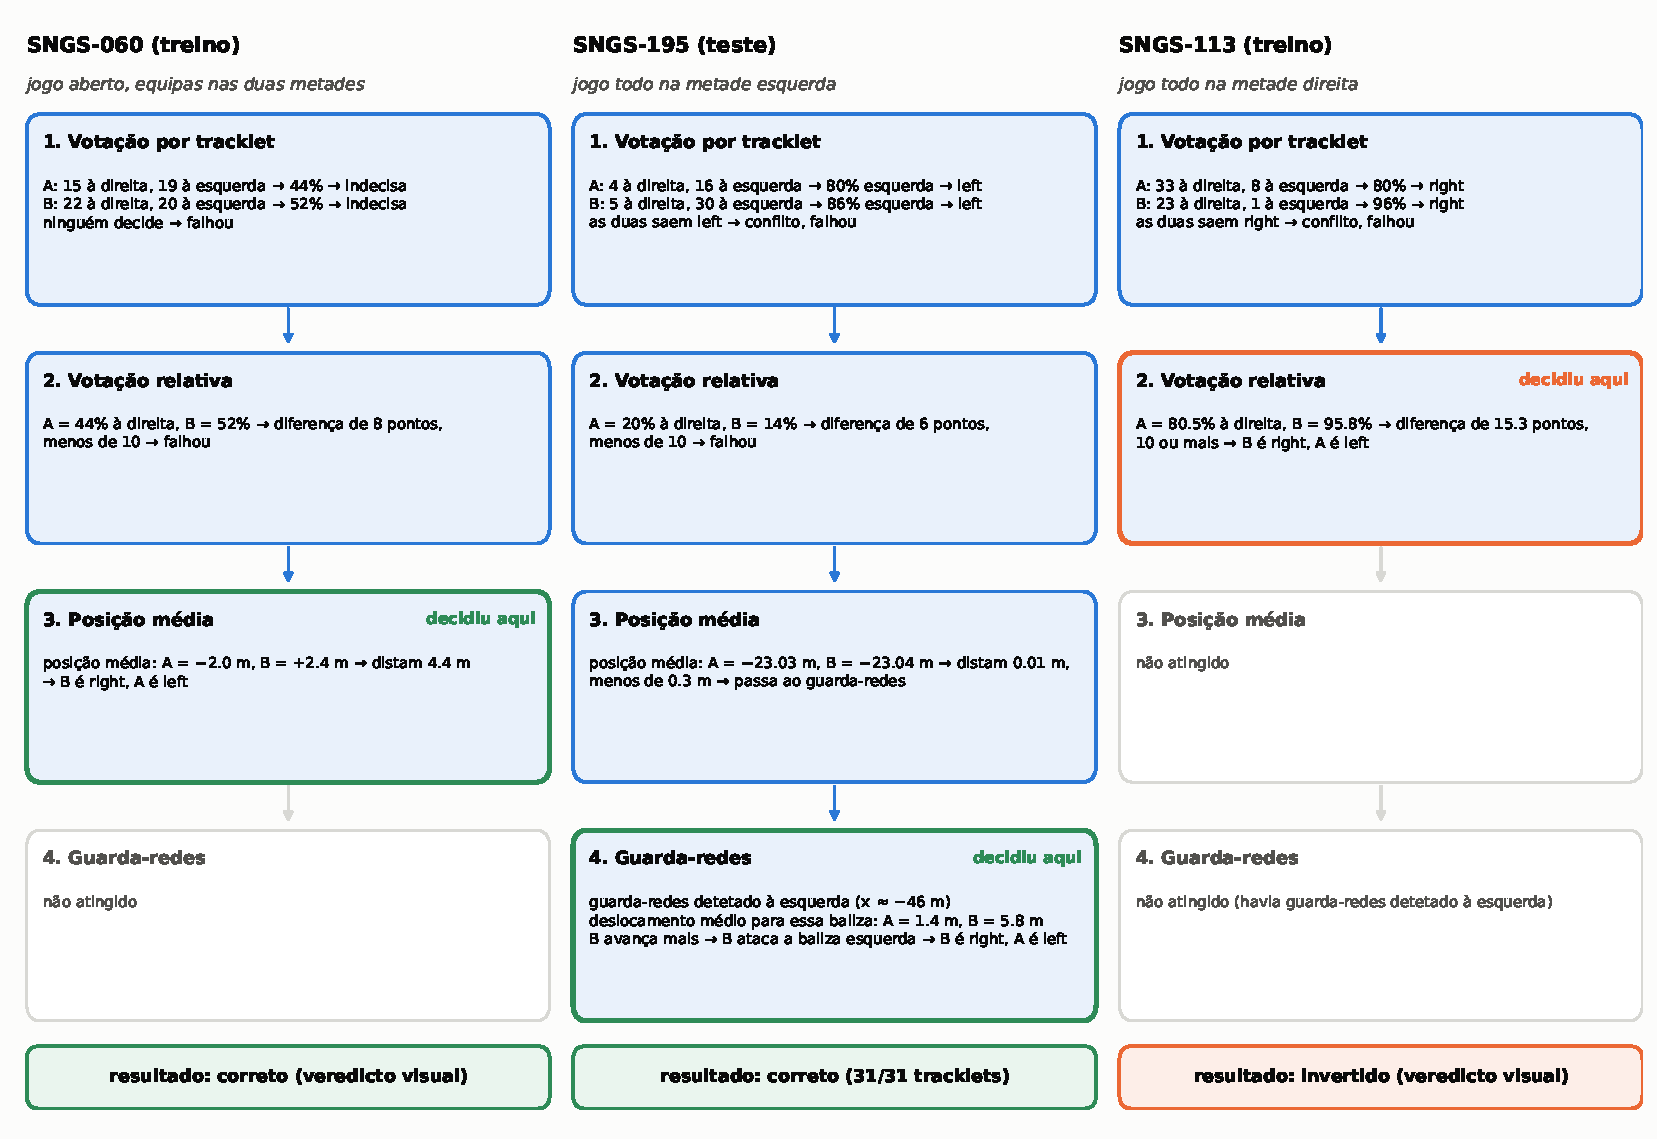
\includegraphics[width=\textwidth]{fig_cascata_exemplos.pdf}
    \caption{A cascata do lado em três vídeos reais, com o critério que decide em cada um e o resultado.}
    \label{fig:cascata-exemplos}
\end{figure}

O SNGS-113 mostra onde a cascata falha. As duas equipas estão na metade direita, com as medianas a apenas $9.7$ metros uma da outra, ao passo que os guarda-redes distam $73.5$ metros (Figura~\ref{fig:113-campo}). Os dois grupos têm a maioria dos \emph{tracklets} na metade direita, $80.5\%$ e $95.8\%$, pelo que a votação por \emph{tracklet} não decide. A votação relativa decide pela diferença de $15.3$ pontos e dá o lado direito a B. O resultado está invertido. Essa diferença corresponde a oito \emph{tracklets} contra um do lado esquerdo, num vídeo com $65$ \emph{tracklets} para cerca de vinte jogadores. São fragmentos de trajetórias, e um jogador que o \emph{tracking} partiu em vários pedaços conta várias vezes. Com as duas equipas na mesma metade, essa diferença é ruído e não um sinal do lado. O guarda-redes, que resolveria o caso sem ambiguidade, só é consultado no fim, e o segundo critério decide antes.

\begin{figure}[H]
    \centering
    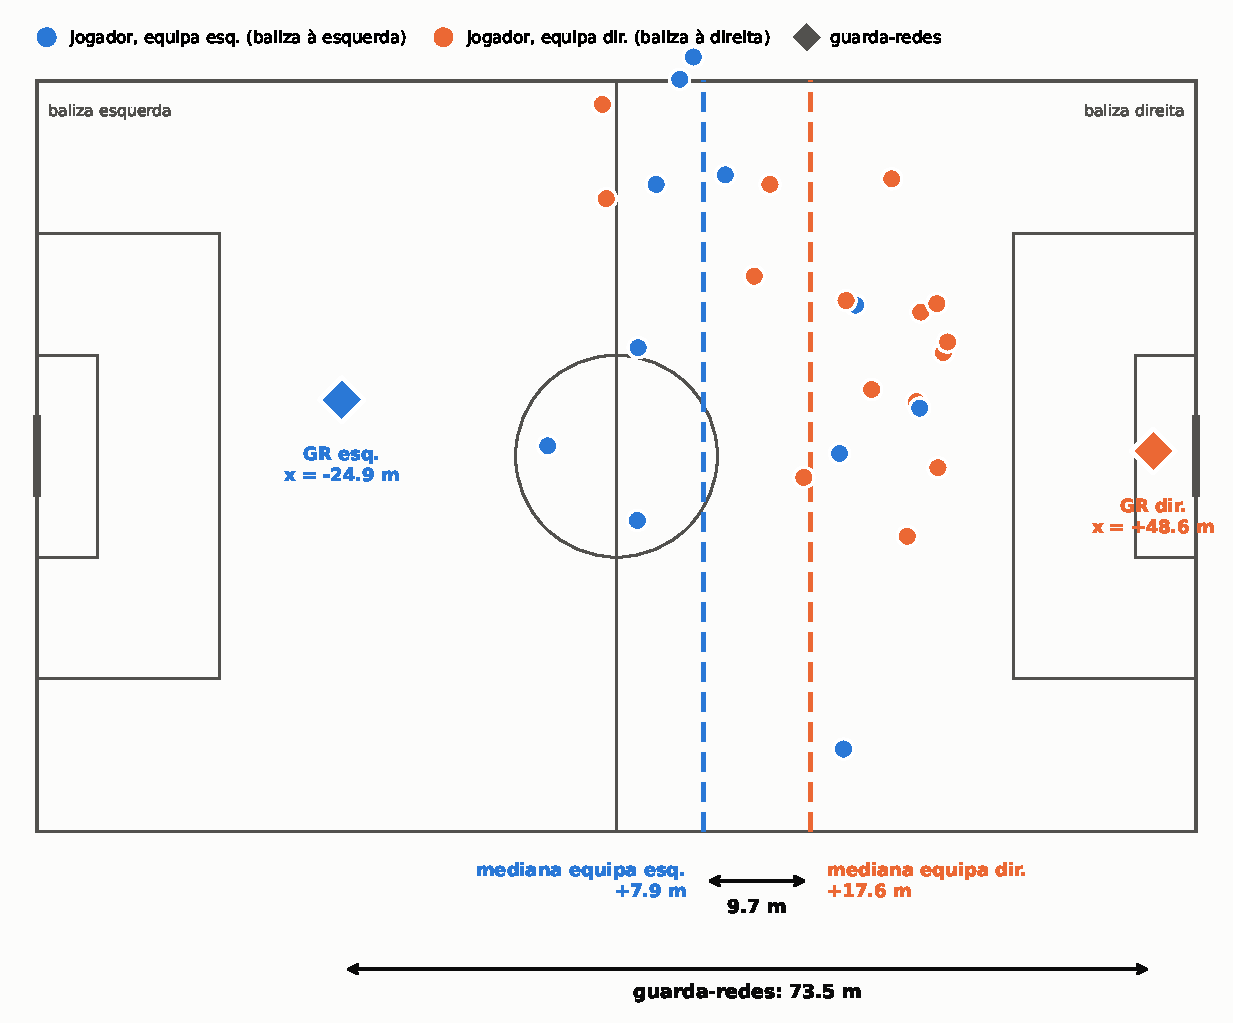
\includegraphics[width=0.9\textwidth]{fig_113_campo.pdf}
    \caption{Anotação de referência do SNGS-113, com a posição mediana de cada jogador. As duas equipas estão na mesma metade e os guarda-redes nos extremos.}
    \label{fig:113-campo}
\end{figure}

A frequência com que cada critério decide mostra que o guarda-redes quase nunca chega a ser consultado. Nos $57$ vídeos de treino, a decisão saiu do primeiro critério em $17$, do segundo em $12$, do terceiro em $28$ e do quarto em nenhum. Nos $39$ vídeos de teste com estado guardado, saiu do primeiro em $5$, do terceiro em $33$ e do quarto em $1$. Na maioria dos vídeos decide, portanto, a comparação de médias da \emph{baseline}, agora protegida pelo filtro dos $60$ metros, e as votações só decidem quando as equipas estão claramente em metades diferentes ou há uma assimetria de pelo menos $10$ pontos. O Capítulo~\ref{cap:resultados} mede, vídeo a vídeo, onde a cascata corrige a \emph{baseline}. O guarda-redes, o sinal mais fiável para esta decisão por não acompanhar as fases de ataque, continua em último lugar, e passá-lo para a frente da cascata fica como a alteração com mais potencial por fazer.

Os limiares da cascata foram recalibrados sobre os conjuntos de teste e de validação em conjunto. A maioria exigida na votação por \emph{tracklet} é de $60\%$, a diferença mínima da votação relativa desceu de $25$ para $10$ pontos e a distância mínima entre médias desceu de $0.5$ para $0.3$ metros. Cada ajuste só foi aceite se resolvia vídeos que falhavam sem estragar nenhum dos que já estavam corretos no conjunto de teste.

\FloatBarrier

\section{Ambiente Experimental}

Esta secção descreve as condições em que o sistema foi desenvolvido e avaliado. Apresenta o ambiente computacional e o conjunto de dados, enumera os hiperparâmetros que governam os módulos alterados e define o procedimento de avaliação sobre o qual assentam os resultados do capítulo seguinte.

\subsection{Ambiente Computacional e Conjunto de Dados}\label{sec:ambiente}

Todo o trabalho foi implementado com base no \emph{framework} TrackLab, responsável pela gestão e execução sequencial dos módulos do \emph{pipeline}, tendo como suporte a biblioteca PyTorch \citep{paszke2019pytorch}. O desenvolvimento decorreu em Python~3.10. A avaliação final, tanto do sistema proposto como da \emph{baseline}, correu num único ambiente em Python~3.12, com as versões das bibliotecas fixadas, de modo que os dois sistemas são comparados nas mesmas condições. A principal restrição computacional decorreu da infraestrutura de \emph{hardware} disponível, um sistema portátil equipado com uma GPU NVIDIA RTX~3060 com apenas 6~GB de VRAM. Esta limitação condicionou várias das decisões metodológicas adotadas, com destaque para a quantização a 4 bits, com recurso à biblioteca \emph{bitsandbytes}, do modelo de visão e linguagem responsável pela leitura do número da camisola (Qwen2.5\babelhyphen{nobreak}VL\babelhyphen{nobreak}3B), e para a gestão explícita da memória de vídeo entre sequências. Como os módulos partilham a mesma GPU, o modelo de visão e linguagem é libertado no fim de cada vídeo. Assim, os pontos do campo e a calibração do vídeo seguinte, que correm antes dele, têm memória disponível. O modelo volta depois a ser carregado do disco, em cerca de cinco segundos.

A avaliação usou o conjunto de dados SoccerNet-GSR, formado por sequências de vídeo de 30 segundos, todas anotadas e divididas em três subconjuntos. São 160 sequências, 57 de treino, 54 de validação e 49 de teste. Uma delas, o SNGS-096 da validação, não pôde ser processada, porque o módulo de calibração falha nesse vídeo nos dois sistemas. A comparação incide, por isso, sobre 159 vídeos. Em cada \emph{frame}, a anotação de referência (\emph{ground truth}) indica a posição de cada interveniente no campo, a sua equipa, a função e o número da camisola. Isto permite avaliar o sistema completo e também cada módulo isoladamente.

O papel de cada subconjunto neste trabalho difere do habitual. Nenhum dos módulos desenvolvidos obriga a treinar modelos, pelo que o subconjunto de treino não foi usado para aprender parâmetros. As regras e os limiares de decisão foram escolhidos sobre os conjuntos de teste e de validação, como se descreve na Secção~\ref{sec:mapeamento}. O conjunto de treino serviu apenas para confirmar cada alteração depois de tomada a decisão. Não é, ainda assim, um conjunto nunca visto. Os seus vídeos foram inspecionados visualmente, como os restantes, e alguns servem de exemplo neste capítulo. A verificação do agrupamento colapsado foi, além disso, desenhada já com os 159 vídeos avaliados. Os resultados do treino mostram, por isso, que as regras se mantêm em vídeos que não serviram para as escolher, mas não equivalem a uma avaliação totalmente cega.


\subsection{Parametrização dos Módulos}

O comportamento dos módulos desenvolvidos é definido por um conjunto de hiperparâmetros, resumidos na Tabela~\ref{tab:hiperparametros}. Os valores relativos ao reconhecimento do número da camisola foram definidos por experimentação, para equilibrar a fiabilidade da leitura com o custo computacional. O limiar de confiança foi escolhido com o GS-HOTA oficial (Secção~\ref{sec:res_jnr_confianca}). Os limiares da atribuição da equipa e do lado do campo resultam da recalibração descrita na Secção~\ref{sec:mapeamento}, conduzida sobre os conjuntos de teste e de validação.


\begin{table}[htbp]
    \centering
    \caption{Hiperparâmetros dos módulos alterados e respetiva função.}
    \label{tab:hiperparametros}
    \footnotesize
    \setlength{\tabcolsep}{4pt}
    \renewcommand{\arraystretch}{0.95}
    \begin{tabular}{|l|l|l|}
        \hline
        \textbf{Parâmetro} & \textbf{Valor} & \textbf{Função} \\
        \hline
        \multicolumn{3}{|l|}{\emph{Reconhecimento do número da camisola (pose e recorte)}} \\
        \hline
        Confiança da pose            & $0.25$          & Deteção mínima dos \emph{keypoints} \\
        \hline
        Alargamento lateral da ROI   & $0.55$          & Margem lateral sobre o tronco \\
        \hline
        Margem superior da ROI       & $0.10$          & Recorte acima dos ombros \\
        \hline
        Fração de altura do tronco   & $0.90$          & Extensão vertical da região dorsal \\
        \hline
        \multicolumn{3}{|l|}{\emph{Reconhecimento do número da camisola (filtro de qualidade)}} \\
        \hline
        Dimensão mínima do recorte   & $15\times20$~px & Rejeita jogadores muito distantes \\
        \hline
        Nitidez mínima               & $15.0$          & Variância do Laplaciano \\
        \hline
        \multicolumn{3}{|l|}{\emph{Reconhecimento do número da camisola (leitura e decisão)}} \\
        \hline
        Modelo de leitura            & Qwen2.5-VL-3B (4 bits) & Inferência do número \\
        \hline
        Recortes por janela          & $6$             & Unidade de decisão temporal \\
        \hline
        Recortes lidos por janela    & $5$             & Os mais nítidos da janela \\
        \hline
        Confiança mínima para votar  & $0.5$           & Produto das probabilidades dos \emph{tokens} \\
        \hline
        \multicolumn{3}{|l|}{\emph{Descritor de cor (reidentificação)}} \\
        \hline
        Atenção mínima do torso      & $0.25$          & Valor mínimo no mapa do tronco do PRTreID (0--1) \\
        \hline
        Píxeis mínimos da máscara    & $16$            & Abaixo, usa a banda central \\
        \hline
        Classes por canal HSV        & $8$             & Três canais, $24$ valores \\
        \hline
        \multicolumn{3}{|l|}{\emph{Atribuição da equipa (agrupamento)}} \\
        \hline
        Limiar de silhueta           & $0.28$          & Abaixo, recorre à cor da camisola \\
        \hline
        Concentração num dos lados   & $0.85$          & Condição do teste complementar \\
        \hline
        Distância entre centros      & $2.04$          & Abaixo, separação por ReID frágil \\
        \hline
        Fração mínima do grupo menor & $0.20$          & Aceitação da alternativa de cor, em \emph{tracklets} e em deteções \\
        \hline
        Dimensão do descritor de cor & $27$            & $24$ do histograma HSV e $3$ da média Lab \\
        \hline
        Deteções mínimas do grupo menor & $0.08$       & Abaixo, partição degenerada e reagrupamento \\
        \hline
        Recortes por \emph{tracklet} (resgate) & $24$  & Amostra uniforme no tempo \\
        \hline
        Região do tronco (resgate)   & $0.6 \times 0.4$ & Fração central da caixa, largura e altura \\
        \hline
        Razão máxima árbitros/jogadores & $0.25$       & Acima, falta uma equipa e não se reagrupa \\
        \hline
        Posição válida (agrupamento) & $|x| \le 52.5$~m & Ignora projeções fora do relvado \\
        \hline
        \multicolumn{3}{|l|}{\emph{Atribuição da equipa (lado do campo)}} \\
        \hline
        Posição válida (lado)        & $|x| \le 60$~m   & Descarta artefactos de calibração \\
        \hline
        Maioria na votação           & $0.60$          & Fração dominante por \emph{tracklet} \\
        \hline
        Diferença relativa mínima    & $0.10$          & Margem do voto relativo \\
        \hline
        Distância mínima entre médias & $0.3$~m        & Abaixo, aciona o desempate pelo guarda-redes \\
        \hline
        Imagens mínimas por \emph{tracklet} & $10$    & Para medir o deslocamento no desempate \\
        \hline
    \end{tabular}
\end{table}


\FloatBarrier
\subsection{Procedimento de Avaliação}\label{sec:protocolo}

A avaliação foi feita em dois níveis, conforme se descreveu na Secção~\ref{sec:metricas}. Para o sistema completo, isto é, com todos os módulos, o desempenho é avaliado e medido pela métrica oficial do desafio, o GS-HOTA. Contudo, para separar o contributo de cada módulo, a métrica é recalculada por fases. Começa-se só com a posição e vai-se juntando, uma de cada vez, a função, a equipa e o número da camisola. Cada atributo que se acrescenta faz a métrica descer, e o tamanho dessa descida mede quanto esse atributo, e logo o módulo que o produz, custa ao resultado final.

O termo de comparação é a \emph{baseline} executada no ambiente de desenvolvimento descrito acima, nos mesmos 159 vídeos, com os módulos originais. Como a deteção, o \emph{tracking} e as representações de reidentificação são partilhados, os \emph{tracklets} avaliados são os mesmos nos dois sistemas e qualquer diferença resulta apenas dos módulos alterados. Para além das métricas automáticas, incluiu-se a inspeção visual dos 159 vídeos de cada sistema, em que cada vídeo é classificado como correto, com o lado trocado, com o agrupamento colapsado numa só equipa, com o agrupamento misturado ou com uma equipa inteira classificada como árbitros. Esta inspeção serve para caracterizar os erros que a métrica agrega e para identificar os vídeos em que a própria anotação de referência está invertida.

A recalibração dos limiares da equipa e do lado seguiu uma regra simples. Cada alteração foi testada nos conjuntos de teste e de validação e só foi aceite se corrigia vídeos que falhavam sem estragar nenhum que a versão anterior já acertava. Esta regra compara cada versão com a anterior e não com a \emph{baseline}. Por isso, o sistema final ainda fica abaixo da \emph{baseline} em 11 vídeos, cinco deles do bloco da equipa de amarelo, como se analisa na Secção~\ref{sec:res_equipa_regressoes}. O conjunto de treino, que não entrou nestes ajustes, permite verificar se os ganhos se mantêm fora dos vídeos usados para os obter. \cleardoublepage
\chapter{Resultados}\label{cap:resultados}

Este capítulo apresenta os resultados dos módulos alterados. O termo de comparação é a \emph{baseline} do desafio SoccerNet-GSR \citep{somers2024soccernet}, executada com os seus módulos originais nos mesmos vídeos e no mesmo ambiente que o sistema proposto. Os dois sistemas partilham a deteção, o \emph{tracking}, a calibração e o modelo de reidentificação. Avaliam, por isso, os mesmos \emph{tracklets}, e as diferenças nos resultados são atribuídas ao que foi alterado. Para que a calibração fosse de facto igual nos dois, a calibração da \emph{baseline} foi refeita com uma homografia por \emph{frame}, pelas razões descritas na Secção~\ref{sec:res_calib_defeito}. A avaliação usa os três subconjuntos anotados, com $49$ vídeos de teste, $53$ de validação e $57$ de treino, $159$ no total. O SNGS-096, da validação, ficou de fora, porque a calibração falha nele nos dois sistemas.

O capítulo começa por avaliar cada módulo individualmente, com uma métrica própria e a inspeção visual descrita na Secção~\ref{sec:protocolo}. Depois, o GS-HOTA mede o efeito das alterações no sistema como um todo. A última secção compara o tempo de execução de cada módulo nos dois sistemas. Nenhuma regra nem limiar foi escolhido com o conjunto de treino, que serviu só para confirmar cada alteração (Secção~\ref{sec:ambiente}).

\section{Reconhecimento do Número da Camisola}\label{sec:res_jnr}

Para avaliar este módulo, conta-se a percentagem de \emph{tracklets} que recebem o número certo, ou seja, a exatidão por \emph{tracklet}. Para isso é preciso saber, primeiro, a que jogador da anotação de referência corresponde cada \emph{tracklet}. Em cada \emph{frame}, cada deteção do \emph{tracklet} fica associada à caixa anotada com que mais se sobrepõe, desde que o IoU seja de pelo menos $0.30$. O IoU (\emph{intersection over union}) é a área da interseção das duas caixas a dividir pela área da sua união. Cada \emph{tracklet} corresponde ao jogador associado em mais \emph{frames}. Por exemplo, se $90$ das $100$ deteções de um \emph{tracklet} coincidirem com o jogador anotado com o $7$, o \emph{tracklet} só está certo se o sistema lhe atribuir o $7$. Um \emph{tracklet} sem número atribuído conta como errado.

Só entram na avaliação os \emph{tracklets} com pelo menos cinco \emph{frames} que correspondem a um jogador com número anotado. Esse jogador tem de estar associado a pelo menos $30\%$ dos \emph{frames} do \emph{tracklet}, para excluir \emph{tracklets} que só de passagem se sobrepõem a ele. Ficam ainda de fora os \emph{tracklets} em que o \emph{tracker} trocou de identidade a meio, isto é, aqueles em que menos de $80\%$ das associações vão para o mesmo jogador. Num \emph{tracklet} que começa no $7$ e acaba no $10$ não há um único número certo. A \emph{baseline} e o sistema proposto são avaliados com estes critérios e sobre os mesmos \emph{tracklets}, pelo que o total avaliado é igual nos dois e a comparação é direta.

\subsection{Resultados}\label{sec:res_jnr_resultados}

Os valores desta secção são os da versão final do módulo. Nesta versão, o Qwen2.5-VL lê o número de cada \emph{tracklet} em janelas de recortes consecutivos, e cada leitura traz a confiança com que o modelo a fez. Só as leituras com confiança de pelo menos $0.5$ contam como voto, e o \emph{tracklet} recebe o número mais votado (Secção~\ref{sec:met-jnr-confianca}). A Secção~\ref{sec:res_jnr_confianca} compara esta versão com a primeira, que não usava a confiança e decidia apenas pela contagem de votos. A Tabela~\ref{tab:jnr} resume os resultados. A exatidão mais do que duplica nos três subconjuntos. Sobe de $19.2\%$ para $46.8\%$ no teste, de $15.8\%$ para $41.8\%$ na validação e de $12.0\%$ para $39.8\%$ no treino. No total dos $159$ vídeos, passa de $15.3\%$ para $42.6\%$. O conjunto de treino não serviu para escolher nenhuma regra nem limiar. Mesmo assim, o ganho nesse conjunto, de $27.8$ pontos percentuais, é da mesma ordem dos obtidos no teste e na validação, onde o módulo foi afinado. A melhoria não depende, portanto, dos vídeos usados para desenvolver o módulo.

\begin{table}[H]
    \centering
    \caption{Exatidão por \emph{tracklet} do reconhecimento do número da camisola, na \emph{baseline} e no sistema proposto, calculada sobre os mesmos \emph{tracklets}. Entre parênteses, os \emph{tracklets} certos sobre o total avaliado.}
    \label{tab:jnr}
    \begin{tabular}{|l|c|c|c|}
        \hline
        \textbf{Conjunto} & \textbf{\emph{Baseline} (MMOCR)} & \textbf{Sistema proposto (Qwen2.5-VL)} & \textbf{$\Delta$} \\
        \hline
        Teste ($49$ vídeos)     & $19.2\%$ ($333/1731$) & $46.8\%$ ($810/1731$)   & $+27.6$ pp \\
        \hline
        Validação ($53$ vídeos) & $15.8\%$ ($267/1691$) & $41.8\%$ ($707/1691$)   & $+26.0$ pp \\
        \hline
        Treino ($57$ vídeos)    & $12.0\%$ ($265/2216$) & $39.8\%$ ($882/2216$)   & $+27.8$ pp \\
        \hline
        Total ($159$ vídeos)    & $15.3\%$ ($865/5638$) & $42.6\%$ ($2399/5638$)  & $+27.2$ pp \\
        \hline
    \end{tabular}
\end{table}

A distribuição dos ganhos por vídeo, na Tabela~\ref{tab:jnr-distribuicao}, mostra que a melhoria não se limita a alguns casos isolados. O sistema proposto melhora em $156$ dos $159$ vídeos, com um ganho mediano de $27.3$ pontos percentuais, e não piora em nenhum. Nos outros três, SNGS-042, SNGS-045 e SNGS-049, todos da validação, os dois sistemas têm exatamente o mesmo resultado.

A diferença vê-se também nos extremos. Na \emph{baseline}, quatro vídeos não têm um único \emph{tracklet} certo (SNGS-106, SNGS-167, SNGS-194 e SNGS-196) e apenas dois chegam aos $50\%$ de exatidão. No sistema proposto, todos os vídeos têm pelo menos um \emph{tracklet} certo e $50$ chegam a esse valor ou ultrapassam-no.

\begin{table}[H]
    \centering
    \caption{Distribuição dos $159$ vídeos pelo ganho de exatidão do reconhecimento do número da camisola face à \emph{baseline}. Ganho em pontos percentuais (pp).}
    \label{tab:jnr-distribuicao}
    \begin{tabular}{|l|c|}
        \hline
        \textbf{Ganho face à \emph{baseline}} & \textbf{N.º de vídeos} \\
        \hline
        Superior a $+40$ pp & $20$ \\
        \hline
        De $+30$ a $+40$ pp & $45$ \\
        \hline
        De $+20$ a $+30$ pp & $48$ \\
        \hline
        De $+10$ a $+20$ pp & $38$ \\
        \hline
        De $+1$ a $+10$ pp  & $5$ \\
        \hline
        Empate ($\pm 1$ pp) & $3$ \\
        \hline
        Regressão           & $0$ \\
        \hline
    \end{tabular}
\end{table}

\subsection{Teto da Abordagem}\label{sec:res_jnr_teto}

A primeira versão do módulo já duplicava a exatidão da \emph{baseline}, mas falhava quase por completo em alguns vídeos. Para perceber se esses casos tinham solução, testaram-se três alterações em seis vídeos, quatro difíceis e dois em que o sistema já funcionava bem, que serviam de controlo. Uma alteração só seria aceite se melhorasse os vídeos difíceis sem piorar os de controlo.

Na primeira alteração, cada janela passou a votar com um peso que crescia com a nitidez, com a área e com a quantidade dos seus recortes. O ganho foi de cerca de um ponto percentual, variou com a forma de calcular os pesos e não mudou nada nos vídeos difíceis. A segunda aplicou aos recortes um realce de contraste por CLAHE (\emph{Contrast Limited Adaptive Histogram Equalization}) antes da leitura. Piorou três vídeos, um deles de controlo, e só melhorou dois. A terceira juntou todos os recortes de um \emph{tracklet} numa única imagem em grelha, para que o modelo combinasse as vistas sozinho, sem votação entre janelas. Melhorou um pouco um vídeo difícil, mas piorou outros, e no total ficou com menos um \emph{tracklet} certo.

As três falharam pela mesma razão. Nos vídeos difíceis, o modelo não lê o número em nenhuma janela, porque os algarismos não se veem nos píxeis, seja pela distância à câmara, seja pela orientação do jogador. Dar mais peso a umas janelas, realçar o contraste ou juntar as vistas não cria essa informação. Além disso, qualquer mudança na imagem de entrada estraga casos que já funcionavam.

Havia ainda um problema que nenhuma delas tocava. Na primeira versão, todas as leituras votavam com o mesmo peso, quer o modelo tivesse visto o número com confiança, quer o tivesse adivinhado num recorte desfocado. Ao escrever a resposta, o modelo atribui uma probabilidade a cada algarismo que gera. O produto dessas probabilidades fica perto de $1$ quando o número é nítido e raramente passa de $0.3$ quando é adivinhado. A informação que faltava não estava na imagem, estava na resposta do modelo. Já existia, mas o sistema descartava-a. A versão final passou a usá-la como confiança da leitura e deixou de contar os votos das leituras pouco seguras (Secções~\ref{sec:met-jnr-confianca} e~\ref{sec:res_jnr_confianca}). O modelo, os recortes e o \emph{prompt} ficaram iguais, e mesmo assim os números errados baixaram de $12.3\%$ para $4.4\%$ das deteções.

\subsection{Contributo da Confiança para a Redução de Erros}\label{sec:res_jnr_confianca}

A exatidão por \emph{tracklet} da Tabela~\ref{tab:jnr} trata todos os \emph{tracklets} por igual. O GS-HOTA, pelo contrário, conta deteções, e um \emph{tracklet} longo com o número errado pesa tanto como muitos \emph{tracklets} curtos juntos. Para perceber onde estava o custo do número na métrica oficial, as deteções de jogadores associadas à anotação foram divididas em cinco categorias (Tabela~\ref{tab:jnr-categorias}). Se o jogador tem número na anotação, o sistema pode acertar nesse número, atribuir outro ou não atribuir nenhum. Se não tem, o sistema acerta quando não lhe atribui nenhum e erra quando lhe atribui um.

Na primeira versão do módulo, sobre os $159$ vídeos, $51.4\%$ das deteções recebiam o número certo, $12.3\%$ um errado e $2.5\%$ um inventado. A maior parte do erro estava em \emph{tracklets} longos. As deteções de \emph{tracklets} com $200$ \emph{frames} ou mais que acabavam com um número errado eram $9.2\%$ do total, três quartos dos $12.3\%$. Para cada \emph{tracklet}, os registos de execução guardam o número que cada janela leu. Com eles foi possível ver, em cada erro, se o número certo tinha sido lido nalguma janela. Em cerca de um terço das deteções com número errado, o certo foi lido nalgumas janelas, mas perdeu a votação para outro que foi lido mais vezes. Nas restantes, o número certo nunca foi lido, e a votação escolheu entre leituras todas erradas. Em ambos os casos, faltava à decisão saber quais das leituras eram seguras.

A decisão pela confiança (Secção~\ref{sec:met-jnr-confianca}) foi testada primeiro numa amostra aleatória de $10$ vídeos de teste e validação, com o mesmo filtro de qualidade da primeira versão. Foi nesta amostra que se escolheu o limiar de $0.5$. Com $0.7$, os números errados desciam ainda mais, mas três vídeos pioravam no GS-HOTA. A versão final junta-lhe o filtro de qualidade mais permissivo descrito na Secção~\ref{sec:met-jnr}. Sem a confiança, esse filtro fazia o sistema inventar números, e com ela passou a ser seguro. A versão final foi depois alargada por fases até cobrir os $159$ vídeos. Umas fases usaram vídeos sorteados e outra usou os cinco de cada conjunto em que a primeira versão mais falhava o número. O treino só entrou nesta altura, já com o limiar fixado. Em cada fase, as duas versões foram comparadas sobre as mesmas deteções, com a mesma anotação e com o GS-HOTA oficial. A Tabela~\ref{tab:jnr-categorias} resume o resultado nos $159$ vídeos.

\begin{table}[H]
    \centering
    \caption{Decisão do sistema sobre o número nas deteções de jogadores, em percentagem ($159$ vídeos).}
    \label{tab:jnr-categorias}
    \begin{tabular}{|l|c|c|c|}
        \hline
        \textbf{O sistema} & \textbf{Primeira versão} & \textbf{Versão final} & \textbf{$\Delta$} \\
        \hline
        Dá o número certo                          & $51.4$ & $57.0$ & $+5.6$ \\
        \hline
        Dá um número errado                        & $12.3$ & $4.4$  & $-7.9$ \\
        \hline
        Não dá número, mas a anotação tem          & $22.9$ & $25.2$ & $+2.3$ \\
        \hline
        Não dá número, e a anotação também não tem & $10.9$ & $12.9$ & $+2.0$ \\
        \hline
        Dá um número, mas a anotação não tem       & $2.5$  & $0.5$  & $-2.0$ \\
        \hline
    \end{tabular}
\end{table}

Os números errados descem para cerca de um terço, de $12.3\%$ para $4.4\%$ das deteções. Os números atribuídos a jogadores sem número na anotação descem de $2.5\%$ para $0.5\%$. Ao mesmo tempo, o número certo sobe $5.6$ pontos percentuais. Pode parecer estranho que uma regra mais exigente acerte mais, mas há duas razões para isso. A primeira é a própria decisão pela confiança. Sem as leituras inseguras na votação, o número certo pode ganhar votações que antes perdia. Na amostra de $10$ vídeos, ainda com o filtro antigo, o número certo já subia de $45.5\%$ para $49.6\%$ das deteções. A segunda é o filtro de qualidade mais permissivo. Como a confiança trava as leituras inseguras, foi possível aceitar recortes mais pequenos e menos nítidos. Parte deles tem um número legível que a primeira versão nem chegava a ver. O preço está nas deteções que ficam sem número apesar de a anotação o ter, que sobem $2.3$ pontos. Pertencem a \emph{tracklets} em que nenhuma janela chegou ao limiar, mesmo quando o número lido estava certo.

No GS-HOTA oficial, a versão final sobe nos três subconjuntos (Tabela~\ref{tab:jnr-confianca-gshota}), incluindo o treino, que não serviu para escolher o limiar. Para a métrica, dar um número errado custa o mesmo que não dar nenhum. Em ambos os casos, a deteção não emparelha com a anotação. Neste atributo, só passam as deteções com o número certo e as que ficam sem ele quando a anotação também não tem nenhum. Na Tabela~\ref{tab:jnr-categorias}, são a primeira e a quarta linhas, que somadas passam de $62.3\%$ para $69.9\%$. Por isso a subida vem quase toda da DetA, que ganha entre $2.4$ e $5.9$ pontos, enquanto a AssA muda menos de um ponto.


\begin{table}[H]
    \centering
    \caption{GS-HOTA oficial com as duas versões do reconhecimento do número (\%).}
    \label{tab:jnr-confianca-gshota}
    \begin{tabular}{|l|c|c|c|}
        \hline
        \textbf{Conjunto} & \textbf{Primeira versão} & \textbf{Versão final} & \textbf{$\Delta$} \\
        \hline
        Teste ($49$ vídeos)     & $43.76$ & $47.87$ & $+4.11$ \\
        \hline
        Validação ($53$ vídeos) & $35.13$ & $36.79$ & $+1.66$ \\
        \hline
        Treino ($57$ vídeos)    & $42.79$ & $45.37$ & $+2.58$ \\
        \hline
    \end{tabular}
\end{table}


A melhoria não é uniforme. O GS-HOTA sobe em $120$ dos $159$ vídeos, desce em $27$ e fica praticamente igual nos restantes $12$. Dos que descem, $13$ perdem menos de um ponto e $9$ mais de dois. A inspeção de vários destes vídeos mostra dois padrões. No primeiro, o modelo lê o número certo várias vezes, mas sempre com pouca confiança. No SNGS-056, um jogador com o número 14 foi lido como 14 em nove de doze janelas, todas com confiança entre $0.3$ e $0.43$. Ficou sem número, quando a primeira versão o acertava. É o custo direto do limiar. No segundo, o modelo troca dígitos parecidos com confiança alta, como o 8 e o 6 ou o 14 e o 16. Estas leituras passam o limiar, e o \emph{tracklet} fica com o número trocado. É o que acontece no SNGS-121 e no SNGS-133, dois vídeos de teste em que a primeira versão já acertava muito.

Há também erros que não são do sistema. No SNGS-188, um \emph{tracklet} lido como 14 com confiança entre $0.6$ e $0.8$ em quase todas as janelas está emparelhado com um jogador anotado com o número 34. Os recortes mostram um 14 legível, e a anotação deste vídeo não tem nenhum 14. No SNGS-187, um jogador com o 14 visível nas costas ao longo de todo o vídeo está anotado sem número. Nestes casos, a métrica conta como erro uma leitura certa.

No extremo oposto, o SNGS-196 mostra o comportamento pretendido. É um vídeo de câmara afastada, com recortes pequenos. Na primeira versão, $9\%$ das deteções recebiam o número certo e $16\%$ um número errado. Na versão final, o número certo sobe para $50\%$, o número errado desaparece e o GS-HOTA do vídeo passa de $17.1$ para $38.7$. Dos quinze jogadores cujo número muda, doze que não tinham nenhum passam a ter o certo. Dois números errados são corrigidos e um terceiro é retirado. Nenhum jogador que estava correto passa a errado.


\subsection{Alternativas Testadas e Rejeitadas}\label{sec:res_jnr_rejeitadas}

Além da decisão pela confiança, testaram-se três correções para outros erros do número. Cada uma atacava uma causa diferente, encontrada ao reavaliar os vídeos. O critério foi sempre o mesmo. Uma correção só entraria no sistema se subisse o GS-HOTA oficial, e não apenas a exatidão por \emph{tracklet}. Nenhuma o conseguiu, mas as três ajudam a perceber onde está o limite do módulo.

\medskip\noindent\textbf{\emph{Tracklets} curtos.} O \emph{tracker} parte muitas vezes um jogador em vários \emph{tracklets}. Os mais curtos têm poucas imagens, e o número sai errado ou fica por ler. A correção testada foi passar o número de um \emph{tracklet} bem lido para os outros \emph{tracklets} do mesmo jogador. Esta experiência foi feita sobre a primeira versão do módulo. Para saber quanto valia no melhor caso, usou-se primeiro a anotação para dizer que \emph{tracklets} são do mesmo jogador. Foi só uma medição, e a anotação não entra no sistema. Nesse caso ideal, a exatidão por \emph{tracklet} subiria de $37.8\%$ para $60.9\%$. Sem a anotação, os grupos têm de ser adivinhados. Juntaram-se os \emph{tracklets} da mesma equipa que nunca aparecem ao mesmo tempo e que o modelo de reidentificação considera parecidos. A exatidão por \emph{tracklet} subiu $5.5$ pontos percentuais, mas o GS-HOTA do conjunto de teste ganhou só $0.04$. Os \emph{tracklets} corrigidos eram curtos, e só $3\%$ das deteções mudaram de número. Além disso, os \emph{tracklets} do grupo continuam separados e passam a contar como identidades diferentes do mesmo jogador. A AssA desceu $0.51$ pontos e anulou quase todo o ganho de $0.35$ na DetA.

\medskip\noindent\textbf{Leituras certas com pouca confiança.} A versão final deixa sem número os \emph{tracklets} em que o certo é lido, mas nunca acima do limiar, como acontece, por exemplo, no vídeo SNGS-056. A correção testada foi usar, só nesses casos, a decisão da primeira versão, desde que pelo menos duas janelas tivessem lido o mesmo número. Numa amostra de $20$ vídeos, o GS-HOTA não subiu. Nos vídeos de teste da amostra, os números atribuídos a jogadores sem número voltaram a aparecer, de $0.1\%$ para $1.1\%$ das deteções. Recuperar estas leituras trazia de volta os erros que o limiar tinha cortado. Testou-se também somar as confianças de cada número em vez de contar as janelas, e o resultado foi o mesmo.

\medskip\noindent\textbf{Números repetidos na mesma equipa.} Dois jogadores da mesma equipa não podem ter o mesmo número ao mesmo tempo. A inspeção visual encontrou casos destes. No SNGS-196, um \emph{tracklet} perde o jogador que seguia, passa para um colega de equipa e leva consigo o número do primeiro. A correção testada foi retirar o número de um dos dois \emph{tracklets} nos \emph{frames} em que o conflito acontece. Uma primeira contagem, em $60$ vídeos, encontrou $107$ conflitos. Em $68$ deles, os dois \emph{tracklets} tinham o número certo. Eram o mesmo jogador, partido em dois \emph{tracklets} que se sobrepunham durante alguns \emph{frames}. Medida em $117$ vídeos, a correção deixou o GS-HOTA igual ou mais baixo nos três subconjuntos, com descidas até $0.15$ pontos. O erro de fundo é uma troca de identidade do \emph{tracker}, que está fora do âmbito deste trabalho, e não se resolve do lado do número.

\medskip\noindent\textbf{O que estas experiências mostram.} Duas das três causas estão no \emph{tracker}, que parte jogadores em vários \emph{tracklets} e troca identidades, e não na leitura. As experiências mostram também que um ganho na exatidão por \emph{tracklet} pode não chegar ao GS-HOTA. A métrica conta deteções, e por isso corrigir \emph{tracklets} curtos quase não se nota. Além disso, avalia as identidades ao longo do tempo, e uma correção certa pode baixá-la, como aconteceu na partilha do número. Por isso, todas as decisões do módulo foram tomadas com o GS-HOTA oficial.


\section{Atribuição da Equipa e do Lado do Campo}\label{sec:res_equipa}

A atribuição da equipa e do lado do campo é avaliada de duas maneiras. A primeira é a exatidão por \emph{tracklet}, com os mesmos critérios usados para o número (Secção~\ref{sec:res_jnr}). Contam só os \emph{tracklets} que o sistema e a anotação classificam como jogadores, e por isso os guarda-redes ficam de fora. A anotação identifica cada equipa pelo lado do campo em que joga. Um \emph{tracklet} só está certo se tiver a equipa e o lado certos. A segunda maneira é a inspeção visual dos $159$ vídeos de cada sistema, em que cada vídeo é classificado numa das cinco categorias da Secção~\ref{sec:protocolo}. São precisas as duas, porque a exatidão por \emph{tracklet} tem pontos cegos. Não conta os \emph{tracklets} que o sistema dá como árbitros nem os que seguem dois jogadores, e por isso não vê alguns erros. Nos vídeos em que a própria anotação está errada, conta como erro o que está certo. O GS-HOTA, analisado na Secção~\ref{sec:desempenho_global}, avalia cada deteção e só partilha este último ponto cego.

\subsection{Resultados}\label{sec:res_equipa_resultados}

A Tabela~\ref{tab:team-conjuntos} mostra a exatidão nos três subconjuntos. Nos $159$ vídeos, a exatidão sobe de $83.5\%$ para $92.8\%$. O ganho está nos dois conjuntos em que a \emph{baseline} mais falhava. No teste sobe de $85.4\%$ para $96.4\%$, e na validação de $66.1\%$ para $86.9\%$. No treino, onde a \emph{baseline} já acertava em $94.5\%$ dos \emph{tracklets}, o sistema proposto fica $0.2$ pontos abaixo.

\begin{table}[H]
    \centering
    \caption{Exatidão da equipa e do lado por \emph{tracklet}, na \emph{baseline} do SoccerNet-GSR e no sistema proposto, sobre os mesmos \emph{tracklets}.}
    \label{tab:team-conjuntos}
    \begin{tabular}{|l|c|c|c|}
        \hline
        \textbf{Conjunto} & \textbf{\emph{Baseline}} & \textbf{Sistema proposto} & \textbf{$\Delta$} \\
        \hline
        Teste ($49$ vídeos)     & $85.4\%$ ($1834/2148$) & $96.4\%$ ($2071/2148$) & $+11.0$ pp \\
        \hline
        Validação ($53$ vídeos) & $66.1\%$ ($1298/1964$) & $86.9\%$ ($1707/1964$) & $+20.8$ pp \\
        \hline
        Treino ($57$ vídeos)    & $94.5\%$ ($2566/2716$) & $94.3\%$ ($2561/2716$) & $-0.2$ pp \\
        \hline
        Total ($159$ vídeos)    & $83.5\%$ ($5698/6828$) & $92.8\%$ ($6339/6828$) & $+9.3$ pp \\
        \hline
    \end{tabular}
\end{table}

Ao contrário do número, o ganho na equipa não é igual em todos os vídeos. O sistema proposto melhora em $44$ vídeos, fica igual em $104$ e piora em $11$. Para simplificar, consideram-se iguais os vídeos com uma diferença de até um ponto percentual. Dos $104$ vídeos iguais, $92$ já estavam a $100\%$ na \emph{baseline}. Das $44$ melhorias, $34$ chegam acima de $95\%$. Nove das dez restantes são vídeos da equipa de amarelo (SNGS-039 a SNGS-058), em que o sistema proposto melhora sem resolver. Os $11$ vídeos que pioram são o resultado que mais importa explicar, e a Secção~\ref{sec:res_equipa_regressoes} analisa-os.

A inspeção visual confirma o mesmo quadro (Tabela~\ref{tab:visual}). Na \emph{baseline}, $111$ dos $159$ vídeos estão corretos. Os restantes têm o lado trocado ($7$), as duas equipas num só grupo ($7$), os grupos misturados ($14$) ou uma equipa inteira classificada como árbitros ($20$). No sistema proposto, $132$ vídeos estão corretos. Sem contar a arbitragem, as falhas do módulo de equipa descem de $28$ para $7$. Ficam $3$ com o lado trocado, $1$ com o agrupamento colapsado e $3$ com um único \emph{tracklet} na equipa errada. Os veredictos da \emph{baseline} foram revistos depois da recalibração descrita na Secção~\ref{sec:res_calib_defeito}, que mudou o resultado em seis vídeos.

\begin{table}[H]
    \centering
    \caption{Classificação visual dos $159$ vídeos de cada sistema.}
    \label{tab:visual}
    \begin{tabular}{|l|c|c|c|c|c|c|}
        \hline
        \textbf{Sistema} & \textbf{Correto} & \textbf{Lado trocado} & \textbf{Colapsado} & \textbf{Misturado} & \textbf{Arbitragem} & \textbf{Anot.\ invertida} \\
        \hline
        \emph{Baseline}  & $111$ & $7$ & $7$ & $14$ & $20$ & $5$ \\
        \hline
        Sistema proposto & $132$ & $3$ & $1$ & $3$  & $20$ & $4$ \\
        \hline
    \end{tabular}
\end{table}

A última coluna da tabela conta os vídeos em que o sistema está certo, mas a anotação oficial tem os lados das duas equipas invertidos. Estes vídeos contam também como corretos. São cinco, o SNGS-126, 131 e 197 no teste, o SNGS-092 na validação e o SNGS-111 no treino. A inspeção visual mostra a inversão, e as posições anotadas confirmam-na. Nos cinco, a equipa anotada como \emph{left} está, em média, $3.8$ a $8.8$ metros mais à direita do que a outra. \citet{oo2026broadcast2pitch} já tinham apontado os três do teste. Os outros dois não aparecem nesse trabalho, que só avalia o teste. Nestes vídeos, quem acerta o lado tem $0\%$ e quem erra tem $100\%$. No SNGS-197, a \emph{baseline} acerta e tem $0\%$, e o sistema proposto erra e tem $100\%$. Por isso, este vídeo conta como lado trocado no sistema proposto. As tabelas mantêm estes vídeos como a métrica os conta, para permitir a comparação com outros trabalhos. Sem eles, a exatidão da equipa passa de $83.5\%$ para $86.1\%$ na \emph{baseline} e de $92.8\%$ para $95.2\%$ no sistema proposto.

A coluna da arbitragem merece também uma nota. Os $20$ vídeos são os da validação SNGS-039 a SNGS-058, em que uma das equipas joga de amarelo. O classificador de função da \emph{baseline}, que este trabalho não alterou, classifica essa equipa como árbitros nos dois sistemas. Os seus \emph{tracklets} ficam de fora do agrupamento, e a equipa e o lado saem errados à partida. Como só contam os jogadores, estes vídeos podem até ter uma exatidão alta. O SNGS-050 tem $100\%$ no sistema proposto, calculados apenas sobre a equipa que sobra. É uma falha comum aos dois sistemas, fora dos módulos alterados, e é a principal razão de a validação ficar abaixo dos outros dois conjuntos nas Tabelas~\ref{tab:team-conjuntos} e~\ref{tab:gshota}. Sem estes $20$ vídeos, a exatidão da equipa do sistema proposto na validação seria de $95.5\%$, e não de $86.9\%$. No GS-HOTA por vídeo, a média destes $20$ vídeos é de $14.2$, contra $48.7$ nos restantes $33$ da validação.

As Figuras~\ref{fig:frames-148} e~\ref{fig:arbitragem-050} mostram um exemplo de cada caso. O SNGS-148 é uma falha da \emph{baseline} que o sistema proposto corrige. No \emph{frame} escolhido, os jogadores de branco atacam a baliza da esquerda e os de vermelho defendem-na. A equipa \emph{left} é, por isso, a de vermelho. A \emph{baseline} separa bem as duas equipas mas troca-lhes o lado. No seu mapa, as cores dos jogadores aparecem trocadas em relação às da anotação. O sistema proposto acerta o lado, e a exatidão da equipa passa de $0\%$ para $100\%$. O SNGS-050 é uma falha comum aos dois sistemas. Os jogadores de amarelo são classificados como árbitros, e só os de verde e branco recebem equipa e lado.

\begin{figure}[H]
    \centering
    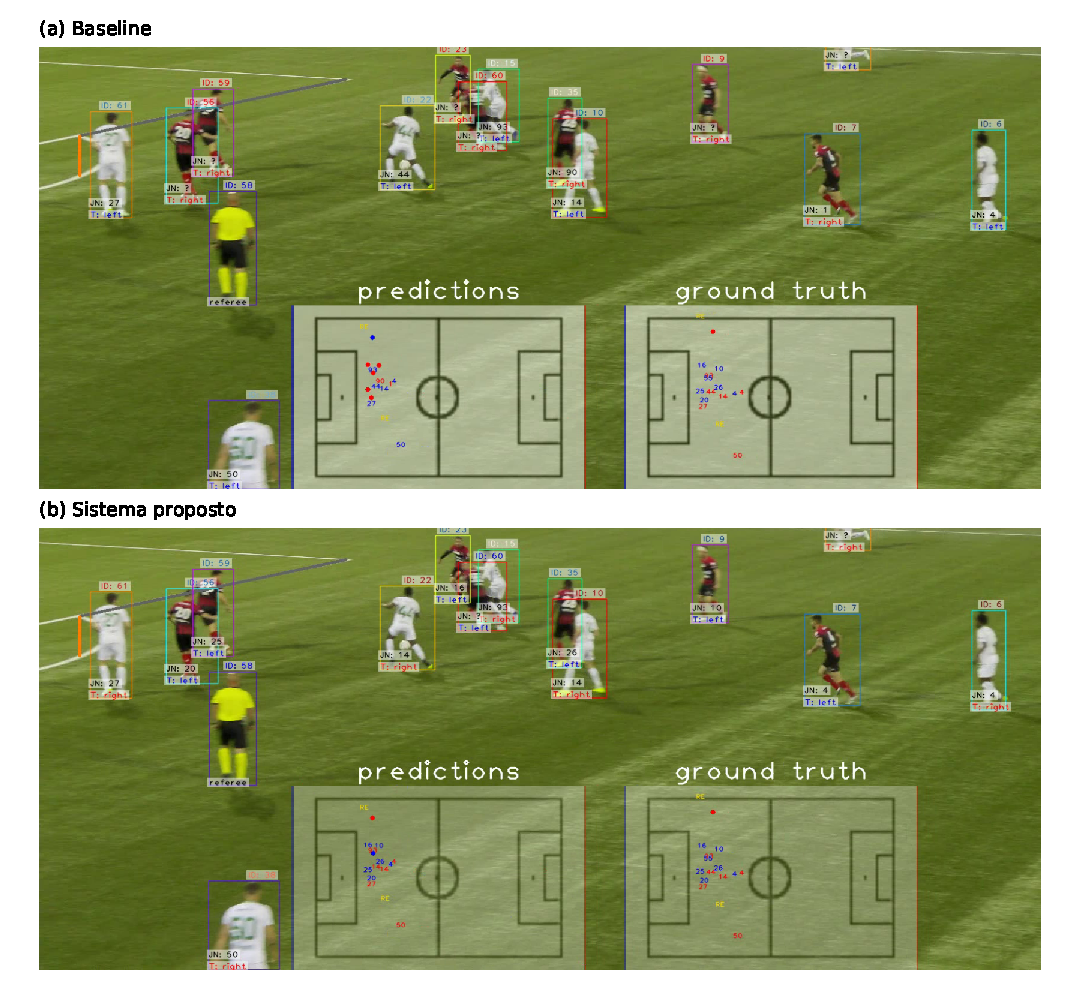
\includegraphics[width=\textwidth]{fig_frames_148.pdf}
    \caption{O mesmo \emph{frame} do SNGS-148 nos dois sistemas, tal como sai do \emph{pipeline}. Em cada mapa, as predições estão à esquerda e a anotação à direita, com \emph{left} a azul e \emph{right} a vermelho.}
    \label{fig:frames-148}
\end{figure}

\begin{figure}[H]
    \centering
    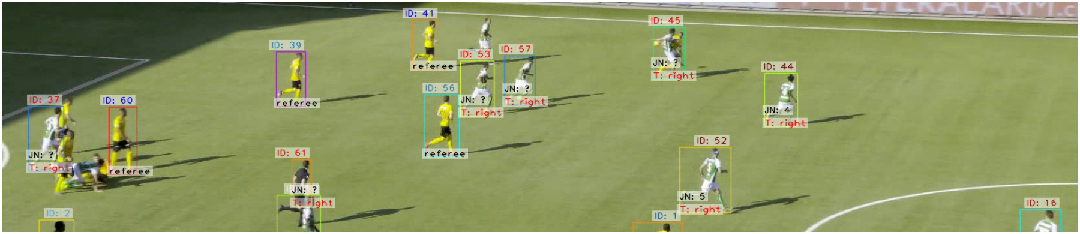
\includegraphics[width=\textwidth]{fig_arbitragem_050.pdf}
    \caption{Função atribuída no SNGS-050 pelo sistema proposto. A \emph{baseline} falha da mesma forma.}
    \label{fig:arbitragem-050}
\end{figure}

\subsection{Contributo de Cada Alteração}\label{sec:res_equipa_ablacao}\label{sec:res_equipa_degenerada}

O módulo de equipa do sistema proposto difere do da \emph{baseline} em três alterações. As duas primeiras foram medidas durante o desenvolvimento, uma de cada vez, sobre os $39$ vídeos de teste usados nessa fase (Tabela~\ref{tab:team-resultados}). A primeira junta o agrupamento pela cor, usado quando o ReID não separa as equipas, e a cascata de votação para o lado (Secções~\ref{sec:agrupamento} e~\ref{sec:mapeamento}). Sozinha, leva a exatidão de $85.4\%$ para $96.1\%$, mas estraga um vídeo, o SNGS-195, que passa de $100\%$ para $0\%$. Neste vídeo, as posições médias das duas equipas diferem apenas $0.01$ metros, e nenhum critério de posição consegue decidir. A segunda alteração, o desempate pelo guarda-redes, repara-o e leva a exatidão a $97.8\%$.

\begin{table}[H]
    \centering
    \caption{Exatidão da equipa e do lado depois de cada alteração, nos $39$ vídeos de teste usados durante o desenvolvimento.}
    \label{tab:team-resultados}
    \begin{tabular}{|l|c|c|}
        \hline
        \textbf{Estado do sistema} & \textbf{Exatidão} & \textbf{$\Delta$} \\
        \hline
        \emph{Baseline}                                   & $85.4\%$ ($1499/1755$) & --- \\
        \hline
        + agrupamento pela cor e cascata de votação       & $96.1\%$ ($1686/1755$) & $+10.7$ pp \\
        \hline
        + desempate pelo guarda-redes           & $97.8\%$ ($1717/1755$) & $+1.7$ pp \\
        \hline
    \end{tabular}
\end{table}

A terceira alteração veio depois, já com os $159$ vídeos avaliados. Nessa versão, o agrupamento tinha uma falha própria. Em onze vídeos, punha quase todos os jogadores no mesmo grupo, como se em campo houvesse uma só equipa. É o agrupamento colapsado da Tabela~\ref{tab:visual}. Nesse caso, só acertam os jogadores do lado atribuído ao grupo grande, e a exatidão fica perto de $50\%$. Em nove dos onze vídeos, ficava entre $43.6\%$ e $61.4\%$.

Esta falha deteta-se sem a anotação. Nos onze vídeos, o grupo menor tinha entre $0.1\%$ e $7.8\%$ das deteções de jogadores. Nos outros $148$, nunca tem menos de $8.7\%$, e a mediana é de $45.8\%$. Há, portanto, uma fronteira clara entre os dois casos, e o próprio módulo pode testá-la.

Posto isto, o módulo passou a verificar cada agrupamento, como descrito na Secção~\ref{sec:agrupamento}. Se o grupo menor tem menos de $8\%$ das deteções de jogadores, o agrupamento é rejeitado. Os \emph{tracklets} são então agrupados de novo pela cor da camisola, medida nas imagens. O novo agrupamento só é aceite se cumprir duas condições. A primeira é que o grupo menor tenha pelo menos $20\%$ dos \emph{tracklets} e das deteções. A segunda é que o classificador de função não classifique como árbitros mais de um quarto dos \emph{tracklets} que dá como jogadores. Se o fizer, falta uma equipa inteira ao agrupamento, e separar por cor o que resta dividiria a outra ao meio.

A Tabela~\ref{tab:regressoes} mostra os onze vídeos em que a verificação dispara. Em cada um, o agrupamento original pôs quase todos os jogadores na mesma equipa, e o grupo menor ficou com menos de $8\%$ das deteções. O SNGS-038 é o caso extremo. O grupo menor tinha só $0.1\%$ das deteções, e o novo agrupamento pela cor dividiu os \emph{tracklets} em $28$ e $16$. A exatidão da equipa passou de $55.2\%$ para $100\%$.

\begin{table}[H]
    \centering
    \caption{Vídeos em que a verificação do agrupamento colapsado dispara.}
    \label{tab:regressoes}
    \begin{tabular}{|l|c|c|c|c|c|}
        \hline
         & \textbf{Agrupamento rejeitado} & \textbf{Novo agrupamento} & \multicolumn{3}{c|}{\textbf{Exatidão da equipa}} \\
        \cline{2-6}
        \textbf{Vídeo} & \textbf{\begin{tabular}[c]{@{}c@{}}Deteções no\\ grupo menor\end{tabular}} & \textbf{\begin{tabular}[c]{@{}c@{}}\emph{Tracklets}\\ por grupo\end{tabular}} & \textbf{\emph{Baseline}} & \textbf{Antes} & \textbf{Depois} \\
        \hline
        SNGS-025 & $3.9\%$ & $33/46$ & $100.0\%$ & $61.4\%$ & $100.0\%$ \\
        \hline
        SNGS-027 & $2.8\%$ & $37/40$ & $52.2\%$ & $47.8\%$ & $100.0\%$ \\
        \hline
        SNGS-028 & $5.9\%$ & $26/27$ & $54.5\%$ & $54.5\%$ & $100.0\%$ \\
        \hline
        SNGS-030 & $0.5\%$ & $31/14$ & $40.0\%$ & $60.0\%$ & $100.0\%$ \\
        \hline
        SNGS-036 & $3.3\%$ & $19/24$ & $96.8\%$ & $51.6\%$ & $100.0\%$ \\
        \hline
        SNGS-038 & $0.1\%$ & $28/16$ & $100.0\%$ & $55.2\%$ & $100.0\%$ \\
        \hline
        SNGS-091 & $7.8\%$ & $33/37$ & $86.7\%$ & $57.8\%$ & $97.8\%$ \\
        \hline
        SNGS-131 & $7.1\%$ & $29/40$ & $0.0\%$ & $43.6\%$ & $0.0\%$ \\
        \hline
        \multicolumn{6}{|l|}{\emph{Novo agrupamento recusado}} \\
        \hline
        SNGS-039 & $5.8\%$ & --- & $21.9\%$ & $0.0\%$ & $0.0\%$ \\
        \hline
        SNGS-050 & $0.8\%$ & --- & $60.9\%$ & $100.0\%$ & $100.0\%$ \\
        \hline
        SNGS-069 & $2.7\%$ & --- & $100.0\%$ & $53.3\%$ & $53.3\%$ \\
        \hline
    \end{tabular}
\end{table}

Em oito vídeos o novo agrupamento é aceite, e a inspeção visual confirma que as duas equipas ficam bem separadas. Seis chegam a $100\%$ e o SNGS-091 a $97.8\%$. O SNGS-131 desce para $0\%$, mas só porque a anotação deste vídeo tem os lados trocados (Secção~\ref{sec:res_equipa_resultados}). Nos outros três, o novo agrupamento é recusado e nada muda. Nos restantes $148$ vídeos, a verificação não dispara.

Os três recusados têm causas diferentes. No SNGS-039 e no SNGS-050, os jogadores de amarelo estão classificados como árbitros. Falta uma equipa ao agrupamento, e a segunda condição impede que a cor divida a outra ao meio. Os $100\%$ do SNGS-050 são enganadores, porque a métrica só avalia a equipa que sobra. No SNGS-069, as equipas jogam de verde e de branco. Ao excluir os píxeis de relva, o descritor de cor apaga também parte das camisolas verdes, e o novo agrupamento volta a ficar desequilibrado. Num ensaio à parte, uma máscara do fundo estimada em cada recorte separou bem as duas equipas, e fica como trabalho futuro.

\subsection{Onde o Sistema Proposto Ainda piora}\label{sec:res_equipa_regressoes}\label{sec:res_equipa_metrica}

Mesmo com as três alterações, o sistema proposto fica abaixo da \emph{baseline} em $11$ vídeos. Cinco são do bloco da equipa de amarelo (SNGS-039, 042, 052, 055 e 057). Aí, os dois sistemas classificam os jogadores de amarelo como árbitros, e o resultado depende de como cada um divide a equipa que fica. Outro é o SNGS-069, o vídeo de verde e branco descrito acima, que continua com o agrupamento colapsado. Há ainda o SNGS-113, com as equipas bem separadas mas o lado trocado. Nos quatro restantes, a diferença é de um a três \emph{tracklets} na equipa errada. Apesar destas descidas, o GS-HOTA sobe em sete dos onze vídeos, e em todos eles o número também melhora.

O SNGS-113 foi analisado na Secção~\ref{sec:mapeamento}. As duas equipas jogam na mesma metade do campo, e o lado é decidido pela votação relativa, o segundo critério da cascata, com uma diferença de $15$ pontos. A média das posições, que a \emph{baseline} usa, acertaria. Mas a cascata só a consulta no terceiro critério, e este vídeo não chega lá.

Por fim, há três vídeos que pioram sem que a métrica o mostre. No SNGS-023 e no SNGS-187, um \emph{tracklet} segue dois jogadores de equipas opostas, quase metade do tempo cada um, e por isso mostra a equipa errada durante parte do vídeo. A exatidão por \emph{tracklet} exclui os \emph{tracklets} que trocam de jogador, e por isso dá $100\%$ aos dois sistemas. No SNGS-197, o sistema proposto troca o lado, e a anotação invertida dá-lhe $100\%$.

\subsection{Robustez do Critério de Atribuição do Lado}\label{sec:res_lado_quantificacao}

Como se viu na Secção~\ref{sec:equipa-desafio}, a maioria das soluções apresentadas ao desafio decide o lado do campo pela posição horizontal média dos jogadores de cada equipa. Nenhuma mede com que frequência esta regra falha. Essa medição foi feita aqui diretamente sobre a anotação, para separar o comportamento da regra dos erros dos outros módulos. Como não depende do sistema, abrange os $160$ vídeos, incluindo o SNGS-096, que fica fora das restantes comparações porque a calibração falha nele.


Compararam-se dois critérios com o lado anotado (Tabela~\ref{tab:lado-inversoes}). O primeiro é a posição do guarda-redes, que não acompanha as fases de ataque e fica junto da sua baliza. Nos $156$ vídeos em que aparece, a sua posição nunca contradiz o lado que lhe foi anotado. O segundo é a posição média dos jogadores de campo de cada equipa. Esta regra discorda da anotação em $7$ dos $160$ vídeos, mas só em dois erra de facto. No SNGS-038 e no SNGS-195, as duas equipas ocupam quase a mesma zona do campo, e as suas posições médias diferem menos de um metro. Os outros cinco são os vídeos com a anotação invertida descritos na Secção~\ref{sec:res_equipa_resultados}. Neles, a regra indica o lado verdadeiro, e é a anotação que está errada. Com a mediana em vez da média, a regra discorda em nove vídeos, porque junta aos sete anteriores o SNGS-056 e o SNGS-130. Usa-se, por isso, a média, que é também a formulação habitual na literatura.

\begin{table}[H]
    \centering
    \caption{Concordância de dois critérios com o lado anotado, nos $160$ vídeos dos três subconjuntos.}
    \label{tab:lado-inversoes}
    \begin{tabular}{|l|c|c|c|}
        \hline
        \textbf{Critério} & \textbf{Vídeos avaliáveis} & \textbf{Discorda da anotação} & \textbf{Dos quais, anotação invertida} \\
        \hline
        Posição do guarda-redes  & $156$ & $0$ & $0$ \\
        \hline
        Posição média da equipa  & $160$ & $7$ ($4.4\%$) & $5$ \\
        \hline
    \end{tabular}
\end{table}

Os dois casos reais mostram o ponto fraco da regra. Quando as duas equipas estão na mesma zona do campo, as médias quase coincidem e a sua ordem deixa de indicar o lado. É este cenário que a cascata da Secção~\ref{sec:mapeamento} trata à parte, primeiro com as votações e, no fim, com o guarda-redes. Ensaiou-se ainda substituir a posição média pelo jogador de campo mais recuado de cada equipa. A ideia é que a última linha defensiva fica entre os atacantes e a sua baliza. Sobre a anotação, este critério só concorda com o lado anotado em $68.6\%$ dos vídeos, contra $95.6\%$ da posição média. A câmara mostra apenas parte do campo, e o jogador mais recuado que se vê nem sempre é o último defesa. A alternativa foi, por isso, posta de parte.

\section{Desempenho Global}\label{sec:desempenho_global}\label{sec:desempenho-global}

O sistema completo é avaliado com o GS-HOTA, a métrica oficial do desafio (Secção~\ref{sec:protocolo}). As secções anteriores mediram cada módulo isoladamente. O GS-HOTA depende também da posição de cada jogador no campo, que vem da calibração da câmara e não faz parte das alterações deste trabalho. Ao calcular o GS-HOTA, encontrou-se na \emph{baseline} um defeito de calibração que piorava as suas posições. Sem o corrigir, parte da diferença entre os dois sistemas seria atribuída ao sistema proposto sem lhe pertencer. A Secção~\ref{sec:res_calib_defeito} descreve o defeito e a sua correção, e as seguintes apresentam os resultados.

\subsection{Correção da Calibração da \emph{Baseline}}\label{sec:res_calib_defeito}

Os dois sistemas usam as mesmas deteções, o mesmo \emph{tracking} e o mesmo código de calibração. Por isso, o GS-HOTA calculado só com a posição, sem os atributos, devia ser igual nos dois. Na primeira avaliação não era. No conjunto de teste, deu $56.7\%$ na \emph{baseline} e $61.8\%$ no sistema proposto. Ao comparar a posição no campo de cada deteção, viu-se que os dois sistemas só coincidiam no primeiro \emph{frame} de cada lote de oito. A causa está na configuração por omissão da \emph{baseline}, que calibra a câmara em lotes de oito \emph{frames}. O módulo de calibração lê os pontos do campo apenas do primeiro \emph{frame} de cada lote e aplica a mesma homografia aos outros sete. Quando a câmara se move dentro do lote, as posições desses sete \emph{frames} ficam erradas. O sistema proposto processa a calibração com lotes de um só \emph{frame}, para caber na memória da placa gráfica junto com o Qwen. Calcula assim uma homografia para cada \emph{frame}, e por isso não tem este defeito.

Para comparar os dois sistemas nas mesmas condições, a calibração da \emph{baseline} foi corrigida da mesma forma, com uma homografia própria para cada \emph{frame} em vez de uma por lote. Os pontos do campo já detetados foram reaproveitados, e só a homografia foi calculada de novo. Com as novas posições, o lado de cada equipa foi depois recalculado com o módulo original da \emph{baseline}. Esta correção não faz parte do sistema proposto nem é um contributo deste trabalho. Serve apenas para que a diferença entre os dois sistemas meça as alterações feitas, e não um defeito de configuração. Todos os valores da \emph{baseline} neste capítulo, incluindo os das Secções~\ref{sec:res_jnr} e~\ref{sec:res_equipa}, são os da versão corrigida. No conjunto de teste, o defeito custava à \emph{baseline} cerca de $5$ pontos no GS-HOTA só com a posição, e $2.4$ na métrica completa. A correção pode, por isso, ser útil a quem use a \emph{baseline} na configuração por omissão, mas esse não foi o seu objetivo.

\subsection{GS-HOTA por Subconjunto}\label{sec:res_gshota}

A Tabela~\ref{tab:gshota} mostra o GS-HOTA dos dois sistemas nos três subconjuntos, com as suas três componentes. A DetA mede a deteção, a AssA a associação ao longo do tempo e a LocA a exatidão da posição. O sistema proposto obtém $47.87\%$ no teste, $36.79\%$ na validação e $45.37\%$ no treino. A \emph{baseline} obtém $31.30\%$, $23.68\%$ e $31.52\%$. Os ganhos são de $16.57$, $13.11$ e $13.85$ pontos.

\begin{table}[H]
    \centering
    \caption{GS-HOTA e componentes nos três subconjuntos. A \emph{baseline} é a versão com a calibração corrigida (Secção~\ref{sec:res_calib_defeito}).}
    \label{tab:gshota}
    \begin{tabular}{|l|l|c|c|c|c|}
        \hline
        \textbf{Conjunto} & \textbf{Sistema} & \textbf{GS-HOTA} & \textbf{DetA} & \textbf{AssA} & \textbf{LocA} \\
        \hline
        \multirow{2}{*}{Teste}     & \emph{Baseline}  & $31.30\%$ & $17.5$ & $56.1$ & $92.8$ \\
        \cline{2-6}
                                   & Sistema proposto & $47.87\%$ & $39.0$ & $58.7$ & $93.3$ \\
        \hline
        \multirow{2}{*}{Validação} & \emph{Baseline}  & $23.68\%$ & $10.3$ & $54.4$ & $91.5$ \\
        \cline{2-6}
                                   & Sistema proposto & $36.79\%$ & $24.5$ & $55.3$ & $92.3$ \\
        \hline
        \multirow{2}{*}{Treino}    & \emph{Baseline}  & $31.52\%$ & $17.9$ & $55.6$ & $92.0$ \\
        \cline{2-6}
                                   & Sistema proposto & $45.37\%$ & $36.3$ & $56.7$ & $92.2$ \\
        \hline
    \end{tabular}
\end{table}

Quase todo o ganho está na DetA, que sobe entre $14.2$ e $21.5$ pontos. A AssA e a LocA mudam menos de $3$ pontos. É o que se espera, porque o GS-HOTA só conta uma deteção como certa se a função, a equipa e o número também estiverem certos. São estes atributos que o sistema proposto melhora, e não a deteção nem a posição, que são iguais nos dois sistemas. O ganho tem a mesma ordem de grandeza nos três subconjuntos, por isso não depende de um subconjunto em particular.

Por vídeo, o ganho mediano é de $15.0$ pontos no teste, $15.5$ na validação e $14.0$ no treino. Só seis vídeos ficam mais de um ponto abaixo da \emph{baseline}. Quatro são regressões da equipa, já descritas na Secção~\ref{sec:res_equipa_regressoes} (SNGS-039, 042, 069 e 113). Os outros dois, o SNGS-043 e o SNGS-049, são do bloco da equipa de amarelo, em que a falha da função domina o resultado dos dois sistemas.

\subsection{Decomposição por Atributo}\label{sec:res_decomposicao}

O GS-HOTA junta todos os módulos num só valor, porque uma deteção só conta se a função, a equipa e o número também estiverem certos. Para separar o efeito de cada atributo, a métrica foi recalculada com os atributos acrescentados um a um. Primeiro conta só a posição no campo, depois junta-se a função, a equipa e, por fim, o número. A última coluna da Tabela~\ref{tab:decomposicao} é, assim, a métrica oficial. A solução vencedora de 2025 fez uma análise parecida (Secção~\ref{sec:jnr-desafio}), mas com cada atributo isolado e só para o seu próprio sistema.

\begin{table}[htbp]
    \centering
    \caption{GS-HOTA com os atributos acrescentados um a um. A última coluna é a métrica oficial.}
    \label{tab:decomposicao}
    \begin{tabular}{|l|l|c|c|c|c|}
        \hline
        \textbf{Conjunto} & \textbf{Sistema} & \textbf{Posição} & \textbf{+ função} & \textbf{+ equipa} & \textbf{+ número} \\
        \hline
        \multirow{2}{*}{Teste}     & \emph{Baseline}  & $61.8$ & $59.4$ & $53.8$ & $31.3$ \\
        \cline{2-6}
                                   & Sistema proposto & $61.8$ & $59.4$ & $57.4$ & $47.9$ \\
        \hline
        \multirow{2}{*}{Validação} & \emph{Baseline}  & $57.7$ & $47.4$ & $38.5$ & $23.7$ \\
        \cline{2-6}
                                   & Sistema proposto & $57.7$ & $47.4$ & $43.0$ & $36.8$ \\
        \hline
        \multirow{2}{*}{Treino}    & \emph{Baseline}  & $58.3$ & $58.2$ & $56.1$ & $31.5$ \\
        \cline{2-6}
                                   & Sistema proposto & $58.3$ & $58.2$ & $55.8$ & $45.4$ \\
        \hline
    \end{tabular}
\end{table}

Só com a posição, os dois sistemas dão o mesmo valor, como têm de dar. Esse valor, entre $57.7\%$ e $61.8\%$, é o máximo que o GS-HOTA pode atingir com a deteção, o \emph{tracking} e a calibração atuais. A função também não foi alterada e custa o mesmo aos dois sistemas. Na validação custa $10.3$ pontos, contra $2.4$ no teste e $0.1$ no treino, por causa dos $20$ vídeos da equipa de amarelo.

A equipa e o número, os dois atributos alterados, são os que afastam os dois sistemas. No teste, a equipa custa $5.6$ pontos à \emph{baseline} e $2.0$ ao sistema proposto. O número tira-lhes $22.5$ e $9.5$. Dos $16.6$ pontos de ganho no teste, $3.6$ vêm da equipa e $13.0$ do número. Na validação, dos $13.1$ pontos, $4.5$ vêm da equipa e $8.6$ do número. No treino, dos $13.9$ pontos, o número dá $14.2$ e a equipa tira $0.3$.

O número é o atributo que mais custa, nos dois sistemas e nos três conjuntos. A única exceção é a validação do sistema proposto, onde a função custa mais do que o número ($10.3$ contra $6.2$ pontos), por causa da equipa com equipamento amarelo. Isto confirma com a métrica oficial o que a solução vencedora de 2025 concluiu sobre o seu sistema, em que o número é também o principal ponto fraco.

\subsection{Enquadramento Competitivo}\label{sec:res_leaderboard}

Os valores deste trabalho não são diretamente comparáveis com a classificação oficial do desafio. Essa classificação é feita no conjunto \emph{challenge}, cuja anotação não é pública, e não nos conjuntos usados aqui. Ainda assim, a Tabela~\ref{tab:leaderboard} dá uma ordem de grandeza, com os três melhores sistemas e a \emph{baseline} oficial de cada edição. A \emph{baseline} oficial de 2025 obtém $29.01\%$ no \emph{challenge}. A mesma \emph{baseline}, corrida neste trabalho na configuração por omissão, obtém $28.95\%$ no teste. Os dois valores são próximos, o que dá alguma confiança na reprodução.

\begin{table}[H]
    \centering
    \caption{Três melhores sistemas e \emph{baseline} oficial das edições de 2024 e 2025, no conjunto \emph{challenge} \citep{cioppa2024soccernet, giancola2025soccernet}.}
    \label{tab:leaderboard}
    \begin{tabular}{|l|c|}
        \hline
        \textbf{Sistema} & \textbf{GS-HOTA} \\
        \hline
        \multicolumn{2}{|l|}{\textit{Edição de 2024}} \\
        \hline
        Constructor Tech  & $63.81\%$ \\
        \hline
        UPCxMobius        & $43.15\%$ \\
        \hline
        JAM               & $34.40\%$ \\
        \hline
        \emph{Baseline} oficial & $23.36\%$ \\
        \hline
        \multicolumn{2}{|l|}{\textit{Edição de 2025}} \\
        \hline
        KIST-GSR          & $63.90\%$ \\
        \hline
        Constructor Tech  & $63.81\%$ \\
        \hline
        lianyou           & $62.76\%$ \\
        \hline
        \emph{Baseline} oficial & $29.01\%$ \\
        \hline
    \end{tabular}
\end{table}

Os sistemas do topo passam os $60\%$ com melhorias em todo o \emph{pipeline}, incluindo a deteção e a calibração. Este trabalho não alterou nenhuma destas duas partes. Só com a posição, antes de contar qualquer atributo, o sistema proposto fica em $61.8\%$ no teste (Tabela~\ref{tab:decomposicao}). Esse é o máximo que pode atingir enquanto a deteção e a calibração forem as da \emph{baseline}.

O sistema proposto tem três pontos em comum com estas soluções. A vencedora de 2025 \citep{oo2026broadcast2pitch} usa um modelo de visão e linguagem, o LLaMA-3.2-Vision, para ler a função, o número e a cor de cada jogador. O sistema proposto faz o mesmo com o Qwen, mas só para o número. O relatório dessa edição \citep{giancola2025soccernet} refere também o Qwen2-VL entre os modelos usados com sucesso para esta leitura. A mesma solução agrupa os jogadores pela cor da camisola, como o sistema proposto. Mas decide o lado pela média das posições, que é a regra da \emph{baseline} que a cascata deste trabalho substitui. Por fim, o recorte do tronco guiado pela pose, que antecede a leitura do número, também aparece noutra solução da edição de 2025.


\section{Custo Computacional}\label{sec:res_tempos}

A Tabela~\ref{tab:tempos} mostra o tempo de cada módulo por vídeo de $30$ segundos ($750$ \emph{frames}), na GPU portátil descrita na Secção~\ref{sec:ambiente}. Os valores são medianas sobre os vídeos processados, medidas pelo cronómetro do próprio motor de execução. O total é de $21.3$ minutos na \emph{baseline} e $22.0$ no sistema proposto, muito longe do tempo real. Nos dois sistemas, a maior parte do tempo vai para a reidentificação, a leitura do número e a deteção dos pontos do campo. A redução deste custo é discutida no Capítulo~\ref{cap:conclusao}.

\begin{table}[htbp]
    \centering
    \caption{Tempo de execução de cada módulo num vídeo de $750$ \emph{frames}, em segundos. Mediana sobre os vídeos processados.}
    \label{tab:tempos}
    \begin{tabular}{|l|c|c|}
        \hline
        \textbf{Módulo} & \textbf{\emph{Baseline}} & \textbf{Sistema proposto} \\
        \hline
        Deteção (YOLOv8)                          & $97.3$  & $96.4$ \\
        \hline
        Reidentificação (PRTreID)                 & $448.7$ & $484.4$ \\
        \hline
        \emph{Tracking} (StrongSORT)              & $31.8$  & $30.9$ \\
        \hline
        Pontos do campo (NBJW)                    & $211.9$ & $210.3$ \\
        \hline
        Calibração (homografia)                   & $5.7$   & $21.5$ \\
        \hline
        Número da camisola (MMOCR / proposto)     & $486.7$ & $477.7$ \\
        \hline
        Voto por \emph{tracklet}                  & $0.1$   & $0.1$ \\
        \hline
        Equipa (agrupamento)                      & $0.7$   & $1.3$ \\
        \hline
        Lado do campo                             & $0.0$   & $0.1$ \\
        \hline
        Total dos módulos                         & $21.3$ min & $22.0$ min \\
        \hline
    \end{tabular}
\end{table}

As alterações deste trabalho acrescentam pouco tempo. No sistema proposto, o reconhecimento do número da camisola demora o mesmo que com o MMOCR, $478$ contra $487$ segundos, apesar de usar um modelo de visão e linguagem. Isto acontece porque só lê os recortes que passam o filtro de qualidade. O agrupamento e o lado do campo somam menos de dois segundos por vídeo. A maior diferença está na reidentificação, que demora mais $36$ segundos porque, no sistema proposto, calcula também o descritor de cor da camisola usado no agrupamento. A calibração passa de $5.7$ para $21.5$ segundos, porque o sistema proposto calcula uma homografia por \emph{frame} e a \emph{baseline} uma por lote de oito (Secção~\ref{sec:res_calib_defeito}).

A decisão pela confiança obrigou ainda a ler cada janela uma segunda vez, para registar as probabilidades dos \emph{tokens}. Esta segunda leitura correu à parte do \emph{pipeline}, não foi cronometrada e não está incluída na tabela. As probabilidades saem da mesma chamada ao modelo que gera a resposta, e por isso podem ser registadas logo na primeira leitura. Numa implementação integrada, este custo desaparece.

\section{Síntese}\label{sec:res_sintese}

Este trabalho alterou quatro dos nove módulos da \emph{baseline}. Substituiu ou reescreveu três, o reconhecimento do número da camisola, a equipa e o lado do campo, e estendeu um, a reidentificação. O ganho é claro e repete-se nos três subconjuntos.

O reconhecimento do número da camisola passa de $15.3\%$ para $42.6\%$ dos \emph{tracklets} nos $159$ vídeos. Melhora em $156$ vídeos e não piora em nenhum. A decisão pela confiança da leitura reduz os números errados a cerca de um terço, de $12.3\%$ para $4.4\%$. A atribuição da equipa e do lado passa de $83.5\%$ para $92.8\%$. Na inspeção visual, os vídeos com falhas deste módulo descem de $28$ para $7$. No GS-HOTA, o ganho é de $16.57$ pontos no teste, $13.11$ na validação e $13.85$ no treino. A decomposição por atributo mostra que todo este ganho vem da equipa e do número, os dois atributos alterados.

A comparação foi feita contra a \emph{baseline} com a calibração corrigida. Sem essa correção, o defeito de calibração custava-lhe cerca de $5$ pontos de GS-HOTA na posição e $2.4$ na métrica completa, que passariam por ganho do sistema proposto.

Os limites também ficaram claros. Nos casos mais difíceis, o número não está visível na imagem devido à distância da câmara ou à orientação do jogador, e nenhuma transformação do recorte o recupera (Secção~\ref{sec:res_jnr_teto}). Na atribuição da equipa, ficam $20$ vídeos em que o classificador de função, que não foi alterado, dá todos os jogadores de amarelo como árbitros. Ficam também três vídeos com o lado trocado, um deles comum aos dois sistemas. Numa versão anterior, o sistema proposto juntava por vezes quase todos os jogadores num só grupo. A verificação da Secção~\ref{sec:res_equipa_degenerada} corrige oito dos onze vídeos em que isso acontecia e não muda nenhum dos outros $148$. \cleardoublepage


% #################### End Chapter and Bibliography ######################
% ALTERADO: removido o \setcounter{secnumdepth}{-1} que aqui estava, para que
% a conclusao seja o Capitulo 5 e apareca numerada.
\chapter{Conclusão}\label{cap:conclusao}

Esta dissertação partiu de uma análise da \emph{baseline} do desafio SoccerNet Game State Reconstruction, que revelou dois pontos fracos na identificação dos jogadores. O primeiro era o reconhecimento do número da camisola, correto em apenas $15.3\%$ dos \emph{tracklets}. O segundo era a atribuição da equipa e do respetivo lado do campo, que falhava em $28$ dos $159$ vídeos avaliados. Foi sobre estes dois problemas que o trabalho se concentrou.

Para os resolver, foram alterados quatro módulos. O módulo de reconhecimento do número da camisola foi substituído, enquanto os módulos de atribuição da equipa e do lado do campo foram reescritos. A reidentificação também foi modificada, mas apenas para calcular um descritor de cor utilizado no agrupamento das equipas, sem alterar o que já produzia. Os restantes cinco módulos foram mantidos idênticos aos da \emph{baseline}. São a deteção, o \emph{tracking}, a estimativa dos pontos do campo, a calibração e a agregação por \emph{tracklet}.

Manter estes cinco módulos inalterados foi uma decisão de método, e não apenas uma delimitação do âmbito do trabalho. Como todos os restantes componentes permaneceram iguais, qualquer diferença de desempenho entre os dois sistemas pode ser atribuída às alterações introduzidas. Com o mesmo objetivo, a \emph{baseline} foi executada nos mesmos $159$ vídeos, no mesmo ambiente e sobre os mesmos \emph{tracklets}. Restava ainda separar o efeito de cada alteração. Para isso, o GS-HOTA foi decomposto por atributo.

É neste ponto que o trabalho se distingue da maioria das soluções apresentadas ao desafio. Estas modificam vários módulos ao mesmo tempo e, por isso, mesmo quando o GS-HOTA sobe muito, é difícil saber quanto do ganho resulta de cada alteração. Nesta dissertação, graças à decomposição por atributo, esse efeito lê-se de forma direta.

No reconhecimento do número da camisola, o OCR da \emph{baseline} foi substituído pelo modelo de visão e linguagem Qwen2.5-VL-3B. Para caber nos 6~GB de memória da placa gráfica, o modelo foi quantizado a 4 bits. A substituição do modelo não foi, contudo, a única alteração. Mudou também a forma como o problema lhe é apresentado, em três passos.

Primeiro, em vez de lhe ser entregue o recorte completo do jogador, isola-se a região do tronco a partir da pose estimada. Depois, descartam-se os recortes sem informação útil. Por fim, o número de cada \emph{tracklet} é decidido apenas com as leituras em que a confiança do modelo, medida pela probabilidade da resposta, passa um limiar.

Este último passo resultou de um diagnóstico da primeira versão do módulo, que tratava todas as leituras como igualmente fiáveis. Com a introdução deste critério, os erros reduziram-se para cerca de um terço, passando de $12.3\%$ para $4.4\%$ das deteções de jogadores, enquanto os acertos aumentaram de $51.4\%$ para $57.0\%$.

Na atribuição da equipa, as alterações abrangeram as duas fases do módulo, o agrupamento dos jogadores em duas equipas e a escolha do lado de cada uma. No agrupamento, quando a reidentificação não consegue distinguir as duas equipas, os jogadores passam a ser agrupados pela cor da camisola. Essa cor é medida na região do tronco, durante a própria reidentificação. O agrupamento também passou a validar o seu resultado. Se uma das equipas ficar com menos de $8\%$ das deteções, o agrupamento é rejeitado e refeito com base na cor.

Na escolha do lado, o critério único da \emph{baseline}, baseado na posição média de cada equipa, deu lugar a uma cascata de quatro critérios, aplicados por ordem até que um deles decida. Cada critério é menos exigente do que o anterior, e o último consiste num desempate pelo guarda-redes.

Os ganhos foram medidos em todos os vídeos anotados, por comparação com a \emph{baseline} executada nas mesmas condições. No número da camisola, a exatidão por \emph{tracklet} subiu de $15.3\%$ para $42.6\%$ nos $159$ vídeos. Houve melhoria em $156$ vídeos e nenhum piorou. Na atribuição da equipa e do lado, a exatidão passou de $83.5\%$ para $92.8\%$ dos \emph{tracklets}. Na inspeção visual, os vídeos em que o módulo de equipa falha desceram de $28$ para $7$.

Na métrica oficial do desafio, o GS-HOTA aumentou $16.57$ pontos no conjunto de teste, de $31.30\%$ para $47.87\%$, $13.11$ na validação e $13.85$ no treino. A decomposição por atributo mostra que todo este ganho resulta dos dois atributos alterados, a equipa e o número. Entre os dois, é o número da camisola que tem maior peso. O ganho é de magnitude semelhante nos três subconjuntos, pelo que não depende de um subconjunto em particular.

Para comparar os dois sistemas, foi ainda necessário corrigir um defeito da \emph{baseline}. O GS-HOTA calculado apenas com base na posição deveria ser igual nos dois sistemas, mas não era. A causa residia na configuração distribuída da \emph{baseline}, que calibra a câmara em lotes de oito \emph{frames} e aplica a homografia do primeiro aos restantes sete. No conjunto de teste, este defeito custava à \emph{baseline} cerca de $5$ pontos de GS-HOTA na posição e $2.4$ pontos na métrica completa. Todos os valores da \emph{baseline} apresentados nesta dissertação correspondem à versão corrigida, de modo a que o ganho reportado resulte apenas das alterações introduzidas. A correção não constitui um contributo deste trabalho, mas pode ser útil a quem utilize a \emph{baseline} na configuração por omissão.

Delimitar o alcance destes ganhos ocupou uma parte importante do trabalho, e começou antes da escolha do modelo. Para a leitura do número, foram comparadas várias abordagens (Tabela~\ref{tab:alternativas}). Entre elas estavam o EasyOCR, o PaddleOCR afinado, o HunyuanOCR, a versão de 7B do Qwen e a super-resolução das imagens. Todas foram postas de parte, porque não liam melhor, não cabiam nos 6~GB da placa gráfica ou eram demasiado lentas.

Já com o Qwen escolhido, foram testadas três formas de melhorar a leitura. A primeira ponderava as leituras pela qualidade do recorte, a segunda realçava o contraste e a terceira juntava todas as vistas de um \emph{tracklet} numa só imagem. Nenhuma melhorou o resultado, e o realce de contraste chegou a piorar vídeos que já estavam certos. As três esbarraram no mesmo obstáculo. Nos casos difíceis, o número não está visível no recorte, pela distância da câmara ou pela orientação do jogador, e nenhuma transformação da imagem o recupera. O que funcionou foi outra via, usar a confiança do modelo para separar as leituras em que viu o número daquelas em que o adivinhou.

Depois disso, foram testadas mais três correções, e todas foram rejeitadas. A fusão de fragmentos do \emph{tracking} subia a exatidão por \emph{tracklet}, mas quase não mudava o GS-HOTA. Recuperar as leituras certas com pouca confiança trazia de volta os números inventados que o limiar tinha cortado. A exigência de que cada número fosse único dentro de cada equipa apagava sobretudo leituras certas, porque a maioria dos conflitos eram fragmentos do mesmo jogador.

Na atribuição da equipa, a inspeção visual dos $159$ vídeos mostra que as falhas que restam têm duas origens. A primeira é o classificador de função, que não foi alterado. Em $20$ vídeos da validação, este classificador dá os jogadores de amarelo como árbitros nos dois sistemas, e essa equipa fica de fora do agrupamento. É isso que deixa a validação abaixo dos outros dois conjuntos. A segunda origem é o próprio módulo de equipa, que ainda erra em sete vídeos, contra $28$ na \emph{baseline}. Em três, o lado está trocado. Nos outros três, há um \emph{tracklet} na equipa errada. No último, as duas equipas ficam num só grupo, porque a verificação do agrupamento não o conseguiu refazer pela cor.

Para perceber até onde a posição dos jogadores indica o lado de cada equipa, analisou-se também a anotação dos $160$ vídeos. Esta análise inclui o SNGS-096, que fica fora da comparação dos sistemas. Em cada vídeo, compararam-se dois critérios com o lado anotado. O primeiro é a posição do guarda-redes, que fica junto à sua baliza e nunca contradiz o lado anotado da sua equipa, nos $156$ vídeos em que aparece. O segundo é a posição média dos jogadores de campo, o critério usado pela generalidade das soluções do desafio. Este falha em sete vídeos, por dois motivos diferentes. Em dois, as duas equipas ocupam quase a mesma zona do campo, e as suas posições médias diferem menos de um metro. Nos outros cinco, o erro está na própria anotação, que dá aos jogadores de campo o lado oposto ao do seu guarda-redes.

Estes cinco vídeos mostram também os limites da métrica de equipa. Neles, um sistema que atribua o lado certo tem $0\%$ de exatidão, porque a anotação diz o contrário. Além disso, a exatidão por \emph{tracklet} não contabiliza os jogadores classificados como árbitros nem os \emph{tracklets} que trocam de jogador, pelo que não capta parte dos erros. Os valores foram mantidos tal como a métrica os conta, para garantir a comparação com outros trabalhos. Ainda assim, uma análise fina desta tarefa exige as duas fontes, a métrica e a inspeção visual.

\section{Trabalho Futuro}\label{sec:trabalho_futuro}

Os resultados apontam para seis linhas de trabalho futuro, apresentadas por ordem de prioridade.

\begin{enumerate}
    \item \textbf{Medição da cor do fundo em cada recorte.} O descritor de cor atual exclui sempre a mesma gama de tons, assumindo que o verde corresponde à relva. Esta suposição falha quando uma das equipas joga com essa cor, como no SNGS-069, de verde e branco. Medir o fundo a partir dos píxeis em redor de cada jogador resolveria este caso. A alteração é local, e os módulos de equipa correm em menos de dois segundos por vídeo.

    \item \textbf{Maior peso do guarda-redes na escolha do lado.} Atualmente, o guarda-redes só entra no último critério de desempate da cascata. No SNGS-113, as duas equipas jogam na mesma metade do campo, mas os dois guarda-redes distam mais de $70$ metros um do outro. Associar cada guarda-redes a um dos grupos permitiria determinar logo o lado correto.

    \item \textbf{Inclusão dos árbitros no agrupamento.} O agrupamento depende hoje do classificador de função para excluir a arbitragem. Em alternativa, poderia procurar cinco grupos, as duas equipas, os árbitros e os dois guarda-redes, à semelhança da solução vencedora de 2024 \citep{golovkin2025minimap}. Esta é a via para os $20$ vídeos da equipa de amarelo, que limitam a validação em ambos os sistemas.

    \item \textbf{Corte dos \emph{tracklets} nas trocas de jogador.} Alguns \emph{tracklets} seguem um jogador e, depois, outro, levando consigo a equipa ou o número do primeiro. Corrigir este problema do lado do número não melhorou a métrica, uma vez que a causa está no \emph{tracking}. A leitura por janela com confiança, que já existe, poderia indicar o ponto de troca, através de uma mudança no número lido com segurança.

    \item \textbf{Redução do custo computacional.} O sistema demora cerca de $22$ minutos por cada $30$ segundos de vídeo, sobretudo na reidentificação, na leitura do número e na estimativa dos pontos do campo. A confiança do modelo pode ser registada logo na primeira leitura, e o número pode ser lido apenas nos \emph{tracklets} que ainda não o têm. A reidentificação pode também ser limitada aos momentos em que o \emph{tracking} é ambíguo.

    \item \textbf{Vídeos de jogos não profissionais.} Os vídeos do SoccerNet-GSR vêm todos de transmissões televisivas de jogos profissionais. Em jogos amadores, a imagem pode ter menos resolução, os equipamentos podem ser menos distintos e o campo pode ter marcações incompletas, o que afeta a calibração. Ensaios preliminares com vídeos amadores, feitos fora desta dissertação, mostraram equipas mal separadas e árbitros dados como jogadores. Avaliar o sistema nestes vídeos, a começar por um conjunto anotado próprio, é o passo necessário para o usar fora do SoccerNet-GSR.
\end{enumerate}

Para além destas linhas, existe uma direção de outra natureza. Considerando apenas a posição, o sistema proposto não ultrapassa os $61.8\%$ de GS-HOTA no conjunto de teste. Os sistemas do topo do desafio ultrapassam os $60\%$ na métrica completa porque melhoram a deteção, o \emph{tracking} e a calibração, os módulos que este trabalho manteve intactos. Este é um âmbito distinto do que aqui foi definido.

Por fim, a direção seguida coincide com a adotada pelas melhores soluções da edição de 2025. A solução vencedora também recorre a um modelo de visão e linguagem para ler o número, o LLaMA-3.2-Vision, cuja versão mais pequena tem $11$ mil milhões de parâmetros. Neste trabalho, chegou-se à mesma ideia de forma independente, com um modelo de $3$ mil milhões de parâmetros que cabe numa placa gráfica de $6$~GB.
 \cleardoublepage

% ALTERADO: a numeracao so e desligada DEPOIS da conclusao, para que a
% bibliografia e os anexos continuem sem numero, como estavam.
\setcounter{secnumdepth}{-1}
%\renewcommand{\bibname}{REFERÊNCIAS BIBLIOGRÁFICAS}

\nocite{*}
\bibliography{Bibliography/references}
 \cleardoublepage

% #################### Attachments ######################
\setcounter{secnumdepth}{-1}
\chapter{Apêndice A. Resultados por Vídeo}\label{anexo:videos}
\setcounter{table}{0}\renewcommand{\thetable}{A.\arabic{table}}

A Tabela~\ref{tab:anexo-videos} reúne os resultados de cada um dos $159$ vídeos nos dois sistemas. Para cada vídeo, mostra a exatidão por \emph{tracklet} da equipa e do número da camisola, o GS-HOTA e o veredicto da inspeção visual.


\setlength{\LTcapwidth}{\textwidth}
\begin{small}
\renewcommand{\tablename}{\normalsize Tabela}
\begin{longtable}{|l|l|r|r|r|r|r|r|l|l|}
\caption{\normalsize Resultados por vídeo. Base.\ é a \emph{baseline} com a calibração corrigida e Prop.\ o sistema proposto. Na coluna Visual, «lado» é o lado trocado, «grupo» o agrupamento colapsado ou misturado, «função» uma equipa classificada como árbitros e «anot. inv.» a anotação com os lados invertidos.}\label{tab:anexo-videos}\\
\hline \textbf{Vídeo} & \textbf{Conj.} & \multicolumn{2}{|c|}{\textbf{Equipa (\%)}} & \multicolumn{2}{|c|}{\textbf{Número (\%)}} & \multicolumn{2}{|c|}{\textbf{GS-HOTA (\%)}} & \multicolumn{2}{|c|}{\textbf{Visual}} \\
 & & Base. & Prop. & Base. & Prop. & Base. & Prop. & Base. & Prop. \\ \hline
\endfirsthead
\hline \textbf{Vídeo} & \textbf{Conj.} & \multicolumn{2}{|c|}{\textbf{Equipa (\%)}} & \multicolumn{2}{|c|}{\textbf{Número (\%)}} & \multicolumn{2}{|c|}{\textbf{GS-HOTA (\%)}} & \multicolumn{2}{|c|}{\textbf{Visual}} \\
 & & Base. & Prop. & Base. & Prop. & Base. & Prop. & Base. & Prop. \\ \hline
\endhead
\hline
\endfoot
SNGS-116 & teste & 100.0 & 100.0 & 34.2 & 55.3 & 38.9 & 44.8 & OK & OK \\ \hline
SNGS-117 & teste & 100.0 & 100.0 & 46.4 & 64.3 & 43.8 & 50.4 & OK & OK \\ \hline
SNGS-118 & teste & 100.0 & 100.0 & 44.4 & 59.3 & 55.0 & 64.3 & OK & OK \\ \hline
SNGS-119 & teste & 100.0 & 100.0 & 52.2 & 82.6 & 66.8 & 86.2 & OK & OK \\ \hline
SNGS-120 & teste & 100.0 & 100.0 & 25.6 & 46.2 & 41.3 & 47.8 & OK & OK \\ \hline
SNGS-121 & teste & 100.0 & 100.0 & 37.8 & 45.9 & 44.3 & 45.8 & OK & OK \\ \hline
SNGS-122 & teste & 100.0 & 100.0 & 20.7 & 34.5 & 27.3 & 34.6 & OK & OK \\ \hline
SNGS-123 & teste & 100.0 & 100.0 & 33.3 & 66.7 & 43.7 & 56.1 & OK & OK \\ \hline
SNGS-124 & teste & 53.8 & 100.0 & 17.9 & 50.0 & 22.9 & 46.2 & grupo & OK \\ \hline
SNGS-125 & teste & 100.0 & 100.0 & 26.5 & 44.1 & 43.3 & 49.1 & OK & OK \\ \hline
SNGS-126 & teste & 0.0 & 0.0 & 75.0 & 93.8 & 20.2 & 20.1 & OK (anot.\ inv.) & OK (anot.\ inv.) \\ \hline
SNGS-127 & teste & 100.0 & 100.0 & 40.0 & 70.0 & 41.2 & 63.2 & OK & OK \\ \hline
SNGS-128 & teste & 100.0 & 100.0 & 24.2 & 51.5 & 37.1 & 58.6 & OK & OK \\ \hline
SNGS-129 & teste & 97.8 & 97.8 & 5.9 & 29.4 & 29.2 & 39.0 & OK & OK \\ \hline
SNGS-130 & teste & 100.0 & 100.0 & 32.3 & 61.3 & 45.1 & 57.9 & OK & OK \\ \hline
SNGS-131 & teste & 0.0 & 0.0 & 23.1 & 38.5 & 18.6 & 18.4 & OK (anot.\ inv.) & OK (anot.\ inv.) \\ \hline
SNGS-132 & teste & 100.0 & 100.0 & 25.0 & 35.7 & 43.7 & 46.7 & OK & OK \\ \hline
SNGS-133 & teste & 100.0 & 100.0 & 25.7 & 65.7 & 28.7 & 35.0 & OK & OK \\ \hline
SNGS-134 & teste & 100.0 & 100.0 & 32.0 & 64.0 & 52.6 & 65.0 & OK & OK \\ \hline
SNGS-135 & teste & 100.0 & 100.0 & 20.6 & 44.4 & 34.4 & 41.7 & OK & OK \\ \hline
SNGS-136 & teste & 97.8 & 100.0 & 27.5 & 42.5 & 43.1 & 47.6 & OK & OK \\ \hline
SNGS-137 & teste & 0.0 & 100.0 & 28.6 & 46.4 & 13.3 & 50.2 & lado & OK \\ \hline
SNGS-138 & teste & 100.0 & 100.0 & 28.8 & 48.1 & 36.9 & 42.7 & OK & OK \\ \hline
SNGS-139 & teste & 100.0 & 100.0 & 20.0 & 33.3 & 27.8 & 40.0 & OK & OK \\ \hline
SNGS-140 & teste & 100.0 & 100.0 & 26.4 & 66.0 & 27.6 & 41.4 & OK & OK \\ \hline
SNGS-141 & teste & 100.0 & 100.0 & 13.0 & 38.9 & 25.0 & 34.7 & OK & OK \\ \hline
SNGS-142 & teste & 100.0 & 100.0 & 14.3 & 28.6 & 27.0 & 37.1 & OK & OK \\ \hline
SNGS-143 & teste & 0.0 & 100.0 & 13.0 & 52.2 & 9.8 & 49.4 & lado & OK \\ \hline
SNGS-144 & teste & 100.0 & 100.0 & 21.3 & 61.7 & 34.1 & 53.5 & OK & OK \\ \hline
SNGS-145 & teste & 100.0 & 100.0 & 10.3 & 24.1 & 27.2 & 43.5 & OK & OK \\ \hline
SNGS-146 & teste & 100.0 & 100.0 & 31.6 & 73.7 & 39.8 & 58.3 & OK & OK \\ \hline
SNGS-147 & teste & 100.0 & 100.0 & 8.3 & 41.7 & 32.9 & 49.0 & OK & OK \\ \hline
SNGS-148 & teste & 0.0 & 100.0 & 18.2 & 59.1 & 13.9 & 40.3 & lado & OK \\ \hline
SNGS-149 & teste & 97.4 & 97.4 & 28.6 & 54.3 & 43.7 & 64.4 & OK & OK \\ \hline
SNGS-150 & teste & 100.0 & 100.0 & 2.4 & 23.8 & 19.0 & 30.1 & OK & OK \\ \hline
SNGS-187 & teste & 100.0 & 100.0 & 15.6 & 53.1 & 21.4 & 46.3 & OK & grupo \\ \hline
SNGS-188 & teste & 100.0 & 100.0 & 8.7 & 43.5 & 34.4 & 53.6 & OK & OK \\ \hline
SNGS-189 & teste & 100.0 & 100.0 & 8.6 & 40.0 & 28.3 & 50.6 & OK & OK \\ \hline
SNGS-190 & teste & 0.0 & 100.0 & 3.4 & 44.8 & 6.4 & 44.7 & lado & OK \\ \hline
SNGS-191 & teste & 100.0 & 100.0 & 2.8 & 38.9 & 14.5 & 47.6 & OK & OK \\ \hline
SNGS-192 & teste & 100.0 & 100.0 & 3.4 & 44.8 & 26.6 & 50.2 & OK & OK \\ \hline
SNGS-193 & teste & 100.0 & 100.0 & 3.3 & 23.3 & 29.1 & 44.1 & OK & OK \\ \hline
SNGS-194 & teste & 100.0 & 100.0 & 0.0 & 50.0 & 18.7 & 59.7 & OK & OK \\ \hline
SNGS-195 & teste & 100.0 & 100.0 & 4.2 & 45.8 & 27.3 & 57.8 & OK & OK \\ \hline
SNGS-196 & teste & 100.0 & 100.0 & 0.0 & 35.6 & 10.1 & 38.7 & OK & OK \\ \hline
SNGS-197 & teste & 0.0 & 100.0 & 14.3 & 50.0 & 10.5 & 56.4 & OK (anot.\ inv.) & lado \\ \hline
SNGS-198 & teste & 100.0 & 100.0 & 7.4 & 42.6 & 17.2 & 39.5 & OK & OK \\ \hline
SNGS-199 & teste & 98.4 & 100.0 & 3.3 & 23.3 & 27.6 & 40.6 & OK & OK \\ \hline
SNGS-200 & teste & 100.0 & 100.0 & 5.3 & 47.4 & 21.2 & 50.6 & OK & OK \\ \hline
SNGS-021 & validação & 100.0 & 100.0 & 26.1 & 47.8 & 41.0 & 50.8 & OK & OK \\ \hline
SNGS-022 & validação & 100.0 & 100.0 & 11.9 & 45.2 & 39.8 & 64.7 & OK & OK \\ \hline
SNGS-023 & validação & 100.0 & 100.0 & 18.9 & 40.5 & 21.4 & 29.0 & OK & grupo \\ \hline
SNGS-024 & validação & 61.0 & 100.0 & 15.4 & 53.8 & 23.7 & 42.5 & grupo & OK \\ \hline
SNGS-025 & validação & 100.0 & 100.0 & 19.0 & 50.0 & 34.3 & 49.0 & OK & OK \\ \hline
SNGS-026 & validação & 56.4 & 100.0 & 20.6 & 50.0 & 30.2 & 57.1 & grupo & OK \\ \hline
SNGS-027 & validação & 52.2 & 100.0 & 8.7 & 26.1 & 19.4 & 37.8 & grupo & OK \\ \hline
SNGS-028 & validação & 54.5 & 100.0 & 20.0 & 60.0 & 13.3 & 46.9 & grupo & OK \\ \hline
SNGS-029 & validação & 0.0 & 100.0 & 9.8 & 46.3 & 13.7 & 48.9 & lado & OK \\ \hline
SNGS-030 & validação & 40.0 & 100.0 & 38.9 & 61.1 & 30.9 & 57.0 & grupo & OK \\ \hline
SNGS-031 & validação & 32.7 & 98.1 & 22.0 & 42.0 & 23.1 & 37.2 & grupo & OK \\ \hline
SNGS-032 & validação & 63.6 & 100.0 & 21.9 & 31.2 & 33.2 & 41.6 & grupo & OK \\ \hline
SNGS-033 & validação & 90.6 & 100.0 & 8.0 & 44.0 & 34.6 & 56.1 & OK & OK \\ \hline
SNGS-034 & validação & 65.8 & 97.4 & 28.9 & 60.5 & 28.9 & 46.4 & grupo & OK \\ \hline
SNGS-035 & validação & 87.7 & 100.0 & 21.2 & 39.4 & 55.4 & 68.2 & OK & OK \\ \hline
SNGS-036 & validação & 96.8 & 100.0 & 14.3 & 52.4 & 39.5 & 57.6 & OK & OK \\ \hline
SNGS-037 & validação & 100.0 & 100.0 & 24.2 & 51.5 & 35.0 & 50.0 & OK & OK \\ \hline
SNGS-038 & validação & 100.0 & 100.0 & 24.1 & 69.0 & 36.5 & 61.9 & OK & OK \\ \hline
SNGS-039 & validação & 21.9 & 0.0 & 6.2 & 18.8 & 19.1 & 4.2 & função & função \\ \hline
SNGS-040 & validação & 20.0 & 91.4 & 2.9 & 11.4 & 3.6 & 10.9 & função & função \\ \hline
SNGS-041 & validação & 17.6 & 17.6 & 11.8 & 29.4 & 14.2 & 17.2 & função & função \\ \hline
SNGS-042 & validação & 96.3 & 88.9 & 7.7 & 7.7 & 16.2 & 5.4 & função & função \\ \hline
SNGS-043 & validação & 12.5 & 87.5 & 3.6 & 10.7 & 14.2 & 12.8 & função & função \\ \hline
SNGS-044 & validação & 65.6 & 65.6 & 8.7 & 21.7 & 14.9 & 16.1 & função & função \\ \hline
SNGS-045 & validação & 34.2 & 68.4 & 13.9 & 13.9 & 6.7 & 11.9 & função & função \\ \hline
SNGS-046 & validação & 75.0 & 92.9 & 7.7 & 30.8 & 6.7 & 35.7 & função & função \\ \hline
SNGS-047 & validação & 11.5 & 11.5 & 7.7 & 23.1 & 4.1 & 5.2 & função & função \\ \hline
SNGS-048 & validação & 26.7 & 26.7 & 10.0 & 70.0 & 16.6 & 16.4 & função & função \\ \hline
SNGS-049 & validação & 10.0 & 90.0 & 18.8 & 18.8 & 19.6 & 8.6 & função & função \\ \hline
SNGS-050 & validação & 60.9 & 100.0 & 4.3 & 47.8 & 12.3 & 19.0 & função & função \\ \hline
SNGS-051 & validação & 62.5 & 75.0 & 18.8 & 25.0 & 4.4 & 18.7 & função & função \\ \hline
SNGS-052 & validação & 71.4 & 28.6 & 4.8 & 33.3 & 13.5 & 17.2 & função & função \\ \hline
SNGS-053 & validação & 15.4 & 84.6 & 12.5 & 62.5 & 4.6 & 29.5 & função & função \\ \hline
SNGS-054 & validação & 64.3 & 67.9 & 3.6 & 39.3 & 1.1 & 8.1 & função & função \\ \hline
SNGS-055 & validação & 80.8 & 69.2 & 4.3 & 17.4 & 1.9 & 2.9 & função & função \\ \hline
SNGS-056 & validação & 0.0 & 57.1 & 45.5 & 72.7 & 9.0 & 13.0 & função & função \\ \hline
SNGS-057 & validação & 75.8 & 45.5 & 3.0 & 33.3 & 0.9 & 9.4 & função & função \\ \hline
SNGS-058 & validação & 56.7 & 56.7 & 3.3 & 33.3 & 6.0 & 21.7 & função & função \\ \hline
SNGS-081 & validação & 53.7 & 90.7 & 31.5 & 55.6 & 16.9 & 43.2 & grupo & OK \\ \hline
SNGS-082 & validação & 71.2 & 100.0 & 25.0 & 46.2 & 23.1 & 41.5 & grupo & OK \\ \hline
SNGS-083 & validação & 26.5 & 98.0 & 16.3 & 41.9 & 26.4 & 56.5 & grupo & OK \\ \hline
SNGS-084 & validação & 69.8 & 98.4 & 8.5 & 33.9 & 18.5 & 31.7 & grupo & OK \\ \hline
SNGS-085 & validação & 81.4 & 100.0 & 20.9 & 51.2 & 25.1 & 53.6 & grupo & OK \\ \hline
SNGS-086 & validação & 95.6 & 100.0 & 14.6 & 56.1 & 29.4 & 46.9 & OK & OK \\ \hline
SNGS-087 & validação & 97.1 & 100.0 & 26.5 & 61.8 & 33.2 & 51.6 & OK & OK \\ \hline
SNGS-088 & validação & 95.0 & 100.0 & 25.0 & 40.6 & 42.7 & 61.1 & grupo & OK \\ \hline
SNGS-089 & validação & 100.0 & 100.0 & 15.9 & 43.2 & 27.9 & 43.4 & grupo & OK \\ \hline
SNGS-090 & validação & 97.8 & 100.0 & 15.6 & 48.9 & 26.8 & 49.8 & OK & OK \\ \hline
SNGS-091 & validação & 86.7 & 97.8 & 9.7 & 41.9 & 24.7 & 42.1 & grupo & OK \\ \hline
SNGS-092 & validação & 0.0 & 0.0 & 13.7 & 33.3 & 16.1 & 16.1 & OK (anot.\ inv.) & OK (anot.\ inv.) \\ \hline
SNGS-093 & validação & 100.0 & 100.0 & 15.2 & 63.0 & 25.3 & 54.3 & OK & OK \\ \hline
SNGS-094 & validação & 71.7 & 100.0 & 22.0 & 51.2 & 35.9 & 52.4 & grupo & OK \\ \hline
SNGS-095 & validação & 97.7 & 100.0 & 10.0 & 43.3 & 35.7 & 59.9 & OK & OK \\ \hline
SNGS-060 & treino & 100.0 & 100.0 & 11.4 & 25.7 & 39.9 & 47.0 & OK & OK \\ \hline
SNGS-061 & treino & 100.0 & 100.0 & 19.0 & 40.5 & 35.5 & 42.8 & OK & OK \\ \hline
SNGS-062 & treino & 100.0 & 100.0 & 18.2 & 42.4 & 38.2 & 53.4 & OK & OK \\ \hline
SNGS-063 & treino & 100.0 & 100.0 & 9.8 & 31.7 & 26.7 & 38.5 & OK & OK \\ \hline
SNGS-064 & treino & 100.0 & 93.0 & 13.9 & 30.6 & 16.4 & 24.1 & OK & OK \\ \hline
SNGS-065 & treino & 100.0 & 100.0 & 14.3 & 45.7 & 34.2 & 51.1 & OK & OK \\ \hline
SNGS-066 & treino & 100.0 & 100.0 & 12.1 & 31.0 & 35.3 & 46.7 & OK & OK \\ \hline
SNGS-067 & treino & 100.0 & 100.0 & 5.3 & 21.1 & 29.1 & 37.8 & OK & OK \\ \hline
SNGS-068 & treino & 68.9 & 95.6 & 8.1 & 32.4 & 23.5 & 50.2 & grupo & OK \\ \hline
SNGS-069 & treino & 100.0 & 53.3 & 28.6 & 39.3 & 41.7 & 33.9 & OK & grupo \\ \hline
SNGS-070 & treino & 100.0 & 100.0 & 28.6 & 42.9 & 36.9 & 48.2 & OK & OK \\ \hline
SNGS-071 & treino & 100.0 & 100.0 & 28.6 & 59.5 & 33.1 & 50.4 & OK & OK \\ \hline
SNGS-072 & treino & 100.0 & 97.7 & 23.3 & 48.8 & 24.3 & 35.9 & OK & OK \\ \hline
SNGS-073 & treino & 100.0 & 100.0 & 10.0 & 33.3 & 38.1 & 53.9 & OK & OK \\ \hline
SNGS-074 & treino & 100.0 & 100.0 & 11.1 & 33.3 & 30.1 & 45.2 & OK & OK \\ \hline
SNGS-075 & treino & 100.0 & 97.7 & 15.0 & 45.0 & 32.6 & 42.1 & grupo & OK \\ \hline
SNGS-076 & treino & 100.0 & 100.0 & 6.7 & 46.7 & 43.7 & 61.2 & OK & OK \\ \hline
SNGS-077 & treino & 100.0 & 97.4 & 16.0 & 32.0 & 51.0 & 64.1 & OK & OK \\ \hline
SNGS-097 & treino & 100.0 & 100.0 & 23.5 & 50.0 & 42.2 & 67.4 & OK & OK \\ \hline
SNGS-098 & treino & 100.0 & 100.0 & 31.2 & 59.4 & 39.4 & 52.7 & OK & OK \\ \hline
SNGS-099 & treino & 100.0 & 100.0 & 5.9 & 44.1 & 37.6 & 48.8 & OK & OK \\ \hline
SNGS-100 & treino & 100.0 & 100.0 & 13.0 & 45.7 & 24.9 & 43.0 & OK & OK \\ \hline
SNGS-101 & treino & 100.0 & 100.0 & 21.1 & 36.8 & 34.8 & 47.6 & OK & OK \\ \hline
SNGS-102 & treino & 100.0 & 100.0 & 15.6 & 31.2 & 34.8 & 44.8 & OK & OK \\ \hline
SNGS-103 & treino & 100.0 & 100.0 & 19.6 & 48.2 & 34.0 & 51.3 & OK & OK \\ \hline
SNGS-104 & treino & 100.0 & 100.0 & 17.9 & 43.6 & 30.4 & 39.4 & OK & OK \\ \hline
SNGS-105 & treino & 100.0 & 100.0 & 12.5 & 37.5 & 32.7 & 51.5 & OK & OK \\ \hline
SNGS-106 & treino & 0.0 & 0.0 & 0.0 & 18.2 & 20.5 & 20.4 & lado & lado \\ \hline
SNGS-107 & treino & 100.0 & 100.0 & 6.7 & 26.7 & 24.4 & 38.4 & OK & OK \\ \hline
SNGS-108 & treino & 100.0 & 100.0 & 6.5 & 41.3 & 28.2 & 46.0 & OK & OK \\ \hline
SNGS-109 & treino & 100.0 & 100.0 & 1.9 & 38.5 & 17.7 & 43.6 & OK & OK \\ \hline
SNGS-110 & treino & 100.0 & 100.0 & 5.7 & 22.6 & 19.1 & 31.9 & OK & OK \\ \hline
SNGS-111 & treino & 0.0 & 0.0 & 6.7 & 50.0 & 16.1 & 16.0 & OK (anot.\ inv.) & OK (anot.\ inv.) \\ \hline
SNGS-112 & treino & 100.0 & 100.0 & 16.7 & 44.4 & 37.0 & 59.4 & OK & OK \\ \hline
SNGS-113 & treino & 100.0 & 0.0 & 19.0 & 57.1 & 34.7 & 16.1 & OK & lado \\ \hline
SNGS-114 & treino & 100.0 & 100.0 & 13.8 & 44.8 & 27.8 & 42.5 & OK & OK \\ \hline
SNGS-115 & treino & 100.0 & 100.0 & 16.7 & 45.2 & 31.2 & 47.5 & OK & OK \\ \hline
SNGS-151 & treino & 100.0 & 100.0 & 17.9 & 42.9 & 39.7 & 52.8 & OK & OK \\ \hline
SNGS-152 & treino & 100.0 & 100.0 & 2.3 & 32.6 & 20.7 & 33.5 & OK & OK \\ \hline
SNGS-153 & treino & 0.0 & 100.0 & 4.5 & 36.4 & 16.9 & 54.9 & lado & OK \\ \hline
SNGS-154 & treino & 100.0 & 100.0 & 11.3 & 37.1 & 23.1 & 35.8 & OK & OK \\ \hline
SNGS-155 & treino & 100.0 & 100.0 & 13.3 & 63.3 & 32.8 & 55.3 & OK & OK \\ \hline
SNGS-156 & treino & 100.0 & 100.0 & 11.9 & 33.3 & 36.5 & 45.3 & grupo & grupo \\ \hline
SNGS-157 & treino & 100.0 & 100.0 & 8.1 & 45.9 & 30.0 & 40.5 & OK & OK \\ \hline
SNGS-158 & treino & 100.0 & 100.0 & 10.0 & 45.0 & 26.5 & 41.4 & OK & OK \\ \hline
SNGS-159 & treino & 100.0 & 100.0 & 5.6 & 20.8 & 21.7 & 29.0 & OK & OK \\ \hline
SNGS-160 & treino & 100.0 & 100.0 & 15.0 & 65.0 & 39.7 & 66.6 & OK & OK \\ \hline
SNGS-161 & treino & 100.0 & 100.0 & 6.2 & 41.7 & 26.0 & 58.9 & OK & OK \\ \hline
SNGS-162 & treino & 100.0 & 100.0 & 2.2 & 28.3 & 29.9 & 43.4 & OK & OK \\ \hline
SNGS-163 & treino & 100.0 & 100.0 & 11.8 & 47.1 & 23.8 & 44.2 & OK & OK \\ \hline
SNGS-164 & treino & 100.0 & 100.0 & 9.3 & 51.2 & 32.3 & 49.4 & OK & OK \\ \hline
SNGS-165 & treino & 100.0 & 100.0 & 25.0 & 55.0 & 45.1 & 62.2 & OK & OK \\ \hline
SNGS-166 & treino & 100.0 & 100.0 & 17.6 & 41.2 & 33.5 & 40.6 & OK & OK \\ \hline
SNGS-167 & treino & 100.0 & 100.0 & 0.0 & 50.0 & 9.9 & 40.4 & OK & OK \\ \hline
SNGS-168 & treino & 100.0 & 100.0 & 5.6 & 33.3 & 32.8 & 50.4 & OK & OK \\ \hline
SNGS-169 & treino & 100.0 & 100.0 & 4.2 & 50.0 & 24.0 & 45.2 & OK & OK \\ \hline
SNGS-170 & treino & 100.0 & 100.0 & 2.2 & 28.3 & 23.9 & 41.9 & OK & OK \\ \hline
\end{longtable}
\end{small}
 \cleardoublepage

\end{document}
